\documentclass[11pt]{article}\usepackage[]{graphicx}\usepackage[]{color}
%% maxwidth is the original width if it is less than linewidth
%% otherwise use linewidth (to make sure the graphics do not exceed the margin)
\makeatletter
\def\maxwidth{ %
  \ifdim\Gin@nat@width>\linewidth
    \linewidth
  \else
    \Gin@nat@width
  \fi
}
\makeatother

\definecolor{fgcolor}{rgb}{0.345, 0.345, 0.345}
\newcommand{\hlnum}[1]{\textcolor[rgb]{0.686,0.059,0.569}{#1}}%
\newcommand{\hlstr}[1]{\textcolor[rgb]{0.192,0.494,0.8}{#1}}%
\newcommand{\hlcom}[1]{\textcolor[rgb]{0.678,0.584,0.686}{\textit{#1}}}%
\newcommand{\hlopt}[1]{\textcolor[rgb]{0,0,0}{#1}}%
\newcommand{\hlstd}[1]{\textcolor[rgb]{0.345,0.345,0.345}{#1}}%
\newcommand{\hlkwa}[1]{\textcolor[rgb]{0.161,0.373,0.58}{\textbf{#1}}}%
\newcommand{\hlkwb}[1]{\textcolor[rgb]{0.69,0.353,0.396}{#1}}%
\newcommand{\hlkwc}[1]{\textcolor[rgb]{0.333,0.667,0.333}{#1}}%
\newcommand{\hlkwd}[1]{\textcolor[rgb]{0.737,0.353,0.396}{\textbf{#1}}}%
\let\hlipl\hlkwb

\usepackage{framed}
\makeatletter
\newenvironment{kframe}{%
 \def\at@end@of@kframe{}%
 \ifinner\ifhmode%
  \def\at@end@of@kframe{\end{minipage}}%
  \begin{minipage}{\columnwidth}%
 \fi\fi%
 \def\FrameCommand##1{\hskip\@totalleftmargin \hskip-\fboxsep
 \colorbox{shadecolor}{##1}\hskip-\fboxsep
     % There is no \\@totalrightmargin, so:
     \hskip-\linewidth \hskip-\@totalleftmargin \hskip\columnwidth}%
 \MakeFramed {\advance\hsize-\width
   \@totalleftmargin\z@ \linewidth\hsize
   \@setminipage}}%
 {\par\unskip\endMakeFramed%
 \at@end@of@kframe}
\makeatother

\definecolor{shadecolor}{rgb}{.97, .97, .97}
\definecolor{messagecolor}{rgb}{0, 0, 0}
\definecolor{warningcolor}{rgb}{1, 0, 1}
\definecolor{errorcolor}{rgb}{1, 0, 0}
\newenvironment{knitrout}{}{} % an empty environment to be redefined in TeX

\usepackage{alltt}

\usepackage{hyperref, lastpage, fancyhdr,multicol,caption,subcaption,tabularx}
\usepackage{amsmath,graphicx}
\usepackage{float}





\topmargin      -1.5cm   % read Lamport p.163
\oddsidemargin  -0.04cm  % read Lamport p.163
\evensidemargin -0.04cm  % same as oddsidemargin but for left-hand pages
\textwidth      16.59cm
\textheight     23.94cm
\parskip         7.2pt   % sets spacing between paragraphs
\parindent         0pt   % sets leading space for paragraphs
\pagestyle{empty}        % Uncomment if don't want page numbers
\pagestyle{fancyplain}

\usepackage{natbib} %need this for bibtex
\IfFileExists{upquote.sty}{\usepackage{upquote}}{}

\lhead{}
\chead{}
\rhead{}

\usepackage{setspace} %for double spacing
\doublespacing
\IfFileExists{upquote.sty}{\usepackage{upquote}}{}
\begin{document}
\begin{knitrout}
\definecolor{shadecolor}{rgb}{0.969, 0.969, 0.969}\color{fgcolor}\begin{kframe}


{\ttfamily\noindent\bfseries\color{errorcolor}{\#\# Error in library(lubridate): there is no package called 'lubridate'}}

{\ttfamily\noindent\bfseries\color{errorcolor}{\#\# Error in library(stargazer): there is no package called 'stargazer'}}

{\ttfamily\noindent\bfseries\color{errorcolor}{\#\# Error in file(file, "{}rt"{}): cannot open the connection}}

{\ttfamily\noindent\bfseries\color{errorcolor}{\#\# Error in file(filename, "{}r"{}, encoding = encoding): cannot open the connection}}\end{kframe}
\end{knitrout}



\title{Energy Balance Measurement Error Models}
\author{Daniel Ries}
\date{\today}
\maketitle

%---------------------------------------------------%
%----------------------%
\section{Introduction}
%----------------------%
%----------------------------------------------------%

We are interested in formulating a model for one's energy balance by using energy expenditure (EE) and changes in energy stores ($\Delta$ ES) while accounting for dependence between the two and measurement error. We can then use this to calculate one's energy intake (EI) via the energy balance equation.   Recall that measuring one's EI is an incredibly hard task, and as such, there is no true accepted gold standard. Because of this, we are using the energy balance principle which states that any energy consumed during a fixed period of time must either be burned (EE) or stored ($\Delta$ES). Fortunately, commonly accepted gold standard measurements exist for both EE (DLW) \cite{lagerros},\cite{bouten},\cite{thomas11},\cite{hall11},\cite{gilmore},\cite{sanghvi15}, \cite{racette11} and $\Delta$ES (DXA) \cite{thomas11},\cite{sanghvi15},\cite{gilmore}. 

In this chapter we take a semi-parametric approach to modeling this problem. We will make distributional assumptions about error terms, but we try to be flexible in modeling the true relationship between cheap measurements and the truth. This analysis requires replicate observations on gold standard and cheap measurements on each individuals, which is expensive and time consuming in terms of data collection, but this method also provides a detailed solution that accounts for all forms of uncertainty.


%-------------------------------------------------------------%
%-------------------------------------------------------------%
\section{Methodology}
%-------------------------------------------------------------%
%-------------------------------------------------------------%


%---------------------------%
\subsection{Notation}
%----------------------------%

We will denote the measured average daily EE by DLW for subject $i$ over time period $j$, $W_{ij}^{EE}$, and average daily change in energy stores measured by DXA for subject $i$ over time period $j$, $W_{ij}^{\Delta ES}$. A positive value for $\Delta$ES indicates that more food was consumed than burned. We are averaging these values because DLW gives an estimate of EE over the course of approximately 14 days, so to keep things simple, we will always talk about average kcals per day. 

We also have cheaper measurements for EE and $\Delta$ES. When collecting data on a large population, it makes more sense to collect these cheaper measurements on most of the subjects. However, they are cheaper for a reason, and ultimately, we would like to use our model assess the measurement error involved and calibrate these cheaper measurements to make them more accurate and precise. Although there are multiple different cheap ways to measure EE and $\Delta$ES, we will keep the notation here general since in any given situation we will be talking only about one specific measurement tool of each. We will denote the measured average daily EE by a cheaper method for subject $i$ over time period $j$, $Y_{ij}^{EE}$, and average daily change in energy stores measured by a cheaper method for subject $i$ over time period $j$, $Y_{ij}^{\Delta ES}$. In application, it will be clear in every situation which tool was used to measure the $Y$'s.

Lastly, the values which we never observe are the \emph{usual} EE and $\Delta$ES for subject $i$. We define \emph{usual} as a long run average of the true EE and $\Delta$ES. Let $X_i^{EE}$ represent the \emph{usual} daily EE for subject i and $X_i^{\Delta ES}$ represent the \emph{usual} daily $\Delta$ES for subject $i$. Note there is considerable within person variability to this \emph{usual} value. However, this value is of not much interest itself. We refer to the \emph{truth} for individual $i$ during time period $j$ as being individual $i$'s \emph{usual} value plus their within person variation during time period $j$ Then:

% \begin{align}
%   \label{trueee}
%   X_i^{EE} &= X_i^{EE} + \delta_{ij}^{EE} \\
%   %
%   \label{truees}
%   X_i^{\Delta ES} &= X_i^{\Delta ES} + \delta_{ij}^{\Delta ES}
% \end{align}

%  Here, $X_i^{EE}$ represents the \emph{true} average daily EE for subject i \emph{over time period j}, and $\delta_{ij}^{EE}$ is the deviation from subject i's \emph{true} average daily EE \emph{over the course of several years} ($X_i^{EE}$) and time j, or in other words, within-person variability. Similarly, $X_i^{\Delta ES}$ is the \emph{true} average daily $\Delta$ES for subject i \emph{over time period j}, and $\delta_{ij}^{\Delta ES}$ is the deviation from subject i's \emph{true} average daily $\Delta$ES \emph{over the course of several years} ($X_i^{\Delta ES}$) at time j. If $X_i^{EI}$ represents subject i at time j's \emph{true} EI, $X_{i}^{EI}$ represents subject i's \emph{usual} EI, and $\delta_{ij}^{EI}$ represents subject i at time j's deviation from his \emph{usual} EI. Then by the energy balance principle:
%  
% \begin{align} 
%   \label{usualebe}
%  X_{i}^{EI} &= X_{i}^{EE} + X_{i}^{\Delta ES} \\
%  X_i^{EI} &= X_i^{EE} + X_i^{\Delta ES} \\
%  \label{withinvar}
%  \delta_{ij}^{EI} &= \delta_{ij}^{EE} + \delta_{ij}^{\Delta ES} 
% \end{align}

%------------------------------%
\subsection{(In)Dependence Assumptions}
%------------------------------%

 Our observed data for subject $i$ over time $j$ will consist of the values ({\bf$W_{ij}^{EE},W_{ij}^{\Delta ES}, Y_{ij}^{EE},Y_{ij}^{\Delta ES}, Z_i$}) where $Z_i$ is a vector of (assumed) perfectly measured covariates for subject $i$. A joint probability model for these observables is represented as:

\begin{align}
  f(W_{ij}^{EE},W_{ij}^{\Delta ES}, Y_{ij}^{EE},Y_{ij}^{\Delta ES}|Z_i,\boldsymbol{\theta})
  \label{fullmodel}
\end{align}

Because of all the dependencies involved, we will deconstruct this via conditional independence assumptions. Given the value $X_i^{EE}$ (\emph{usual} daily EE for subject $i$) and $X_i^{\Delta ES}$ (\emph{usual} daily $\Delta$ES for subject $i$), and covariates $Z_i$, we believe it is reasonable to assume that:

\begin{enumerate}
\item
$Y_{ij}^{EE}$ and $Y_{ij}^{\Delta ES}$ are independent of each other and 
\item
$Y_{ij}^{EE}$ and $Y_{ij}^{\Delta ES}$ are each independent from both $W_{ij}^{EE}$ and $W_{ij}^{\Delta ES}$
\item
$W_{ij}^{EE}$ and $W_{ij}^{\Delta ES}$ are independent of each other

Additionally, given that the above assumptions are reasonable, we expand these by additionally assuming

\item
Given only $X_i^{EE}$ and $Z_i$, $Y_{ij}^{EE}$ and $Y_{ij}^{\Delta ES}$ are independent of each other and from both $W_{ij}^{EE}$ and $W_{ij}^{\Delta ES}$ and vice versa for $\Delta$ES
\item
Given only $X_i^{EE}$ and $Z_i$, $W_{ij}^{EE}$ is independent from $W_{ij}^{\Delta ES}$ and vice versa for $\Delta$ES

\end{enumerate}

 This is because  (1): given the true values \emph{X} and covariates \emph{Z}, knowing a cheap measurement one will give you no more information about the cheap measurement of the other, so long as it is not self-administered. And (2): once we know the truth \emph{X}, having an unbiased measurement of \emph{X} will not provide any more information to the cheap, biased measurement of \emph{X}. DLW and DXA are conducted by separate personnel and these are done separately from those administering the cheap measurement methods. (3) follows the same lines as (1), and again, DXA and DLW are performed by different people.

We are comfortable with conditional independence assumptions (1)-(3) and their validity will not be discussed again. The last two conditional independence assumptions are not as clear cut. It does seem possible that the true change in body composition ($\Delta$ES) could affect how well an activity monitor records EE, even after knowing the true EE and covariates. It also seems possible, but slightly less likely that the same is true for the gold standard measurements. We need to remember this assumption when making conclusions later on.

%----------------------------------%
\subsection{Model Likelihood}
%----------------------------------%

Based on the assumptions made in the previous paragraphs, we can specify our full model \eqref{fullmodel} by:

\begin{align}
  \begin{split}
    \label{truedist}
  f({ W_{ij}^{EE},W_{ij}^{\Delta ES}, Y_{ij}^{EE},Y_{ij}^{\Delta ES}|Z_i},\boldsymbol{\theta}) &= \int \int f({ W_{ij}^{EE},W_{ij}^{\Delta ES}, Y_{ij}^{EE},Y_{ij}^{\Delta ES}, X_i^{EE}, X_i^{\Delta ES}|Z_i},\boldsymbol{\theta}) d{ X_i^{EE}} d{ X_i^{\Delta ES}} \\
  %
    &= \int_{\mathcal{X}_{es}} \int_{\mathcal{X}_{ee}} f({ W_{ij}^{EE}|X_i^{EE},X_i^{\Delta ES},Z_i},\boldsymbol{\theta_{wee}}) f({ W_{ij}^{\Delta ES}|X_i^{EE},X_i^{\Delta ES},Z_i},\boldsymbol{\theta_{wes}}) \times\\
  & f({ Y_{ij}^{EE}|X_i^{EE},X_i^{\Delta ES},Z_i},\boldsymbol{\theta_{yee}}) f({ Y_{ij}^{\Delta ES}|X_i^{EE},X_i^{\Delta ES},Z_i},\boldsymbol{\theta_{yes}}) \times  \\
  & f({ X_i^{EE}, X_i^{\Delta ES}|Z_i},\boldsymbol{\theta_x}) d{ X_i^{EE}} d{ X_i^{\Delta ES}} \\
  %
  &= \int_{\mathcal{X}_{es}} \int_{\mathcal{X}_{ee}} f({ W_{ij}^{EE}|X_i^{EE},Z_i},\boldsymbol{\theta_{wee}}) f({ W_{ij}^{\Delta ES}|X_i^{\Delta ES},Z_i},\boldsymbol{\theta_{wes}}) \times\\
  & f({ Y_{ij}^{EE}|X_i^{EE},Z_i},\boldsymbol{\theta_{yee}}) f({ Y_{ij}^{\Delta ES}|X_i^{\Delta ES},Z_i},\boldsymbol{\theta_{yes}}) \times  \\
  & f({ X_i^{EE}, X_i^{\Delta ES}|Z_i},\boldsymbol{\theta_x}) d{ X_i^{EE}} d{ X_i^{\Delta ES}} 
  \end{split}
\end{align}

Further, we specify the models for the \emph{W}'s and \emph{Y}'s as:

\begin{align}
  \label{regressionfcn1} 
  Y_{ij}^{EE} &= m_{ee}(X_i^{EE} ,Z_i) + \epsilon_{ij}^{EE}  \\
  %
  \label{regressionfcn2}
  Y_{ij}^{\Delta ES} &= m_{es}(X_i^{\Delta ES} ,Z_i) + \epsilon_{ij}^{\Delta ES} \\
  %
  \label{gold1} 
  W_{ij}^{EE} &= X_i^{EE}  + \nu_{ij}^{EE}  \\
  %
  \label{gold2}
  W_{ij}^{\Delta ES} &= X_i^{\Delta ES}  + \nu_{ij}^{\Delta ES} 
\end{align}

where $m_{ee}(\cdot)$ and $m_{es}(\cdot)$ are assumed to be general, smooth functions. $\nu_{ij}^{EE}$ and $\nu_{ij}^{\Delta ES}$ represent the measurement error for subject $i$ during time period $j$ using DLW and DXA, respectively, and within person variability. For now, we let $\epsilon_{ij}^{EE}$ and $\epsilon_{ij}^{\Delta ES}$ represent the measurement error for subject $i$ during time period $j$ using cheap measurements of EE and $\Delta$ES, respectively, and within person variability. This is a working assumption since the within person variability is in reality not an additive error, rather it is added to the usual and realized through the functions $m_{\cdot}(\cdot)$. We cannot directly estimate both within person variability and measurement error simultaneously due to realistic data constraints.  We assume the expected values of all $\epsilon,\nu$ are 0. This implies we are assuming DLW and DXA are providing unbiased estimates for the \emph{usual} daily EE ($X_i^{EE}$) and $\Delta$ES ($X_i^{\Delta ES}$), respectively, and the cheap measurements are giving biased estimates of (possibly) unknown form.


We will assume subjects in the study will have no influence on each other in terms of consumption or exercise behavior, and thus subjects are assumed to be independent of each other. Additionally, conditional on each subjects' respective \emph{usual} value $X_i^{\cdot}$, replicate measurements within subject are independent. Independence within individuals is justified because it is conditional \emph{on each individuals usual value}, which means once we know an individual's baseline, we expect variation from their to be independent day to day. The likelihood function for an individual can then be written as:

\begin{align}
  L_i(\boldsymbol{\theta}) &= \prod_{j=1}^{J} f(W_{ij}^{EE},W_{ij}^{\Delta ES}, Y_{ij}^{EE},Y_{ij}^{\Delta ES}|Z_i,\boldsymbol{\theta}) 
\end{align}

where the RHS is expanded in \eqref{truedist}. Given the independence assumptions in the previous paragraph,  the full likelihood is

\begin{align}
  L(\boldsymbol{\theta}) &= \prod_{i=1}^{n}  L_i(\boldsymbol{\theta}) 
\end{align}



%-------------------------------------
%-------------------------------%
%\section{Models}
%-------------------------------%
%-----------------------------------------

%-------------------------------
\subsection{N{\"a}ive Model}
%-------------------------------

The first model we will consider is what we call the n{\"a}ive model. This model will assume no measurement error in the gold standard instrument exists,  thus DLW and DXA give error-free measurements of $X_i^{EE}$ and $X_i^{\Delta ES}$, respectively. We also assume the cheap measurements $Y$ are linearly related to measurements of the \emph{truth} and of error free covariates. Based on empirical evidence from EBS data, gender, BMI, and age all had some effect on the cheap measurement of EE.  Mathematically, the n{\"a}ive model is represented as:

\begin{align}
Y_{ij}^{EE} &= \beta_{0,ee} + \beta_{1,ee}W_{ij}^{EE}+ \boldsymbol{\gamma_{ee}}Z_i + \epsilon_{ij}^{EE} \\
Y_{ij}^{\Delta ES} &= \beta_{0,es} + \beta_{1,es}W_{ij}^{\Delta ES}+ \boldsymbol{\gamma_{es}}Z_i + \epsilon_{ij}^{\Delta ES} 
\end{align}

where the $\beta_{1,\cdot}$ terms represents the relationship between cheap measurements and the \emph{truth} EE and $\Delta$ES and the $\beta_0$ terms represent systematic biases. $\boldsymbol{\gamma_{\cdot}}=(\gamma_{1,\cdot},\gamma_{2,\cdot},\gamma_{3,\cdot})$ and $\gamma_{1,\cdot}$ is the coefficient for gender, $\gamma_{2,\cdot}$ is the coefficient for BMI, and $\gamma_{3,\cdot}$ is the coefficient for age. We take the standard approach and assume Normal distributions for the error terms, as well as assuming independence within and across individuals conditional on subject $i$:

\begin{align}
  \label{ymodel0}
  (Y_{ij}^{EE} | W_{ij}^{EE},Z_i,\boldsymbol{\theta_{yee}}) &\overset{iid}{\sim} N(\beta_{0,ee} + \beta_{1,ee}W_{ij}^{EE}+ \boldsymbol{\gamma_{ee}}Z_i,\sigma_{\epsilon^{EE}}^2) \\
  \label{ymodel0b}
  (Y_{ij}^{\Delta ES} | W_{ij}^{\Delta ES},Z_i,\boldsymbol{\theta_{yes}}) &\overset{iid}{\sim} N(\beta_{0,es} + \beta_{1,es}W_{ij}^{\Delta ES}+ \boldsymbol{\gamma_{es}}Z_i,\sigma_{\epsilon^{\Delta ES}}^2)
\end{align}

Priors are assumed independent and are assigned below. We chose forms for piors to be conjugate or conditionally conjugate for ease of implementation but also to incorporate weak information. 

\begin{multicols}{2}
\noindent 
\begin{align}
p(\beta_{0,ee}) &\sim N(M_{\beta_{0,ee}},C_{\beta_{0,ee}}) \\
p(\beta_{1,ee}) &\sim N(M_{\beta_{1,ee}},C_{\beta_{1,ee}}) \\
p(\gamma_{g,ee}) &\sim N(M_{\gamma_{ee}},C_{\gamma_{ee}}), \text{ } g=1,2,3 \\
p(\sigma^2_{\epsilon^{ee}}) &\sim IG(a_{yee},b_{yee}) 
\end{align}
\columnbreak
\begin{align}
p(\beta_{0,es}) &\sim N(M_{\beta_{0,es}},C_{\beta_{0,es}}) \\
p(\beta_{1,es}) &\sim N(M_{\beta_{1,es}},C_{\beta_{1,es}}) \\
p(\gamma_{g,es}) &\sim N(M_{\gamma_{es}},C_{\gamma_{es}}), \text{ } g=1,2,3 \\
p(\sigma^2_{\epsilon^{es}}) &\sim IG(a_{yes},b_{yes}) 
\end{align}
\end{multicols}

$\sigma^2_{\epsilon^{ee}}$ and $\sigma^2_{\epsilon^{es}}$ represent the measurement error and within-person variability as measured in the cheap EE and $\Delta$ES tools, respectively. 


%----------------------------------------
\subsection{Linear Measurement Error Model}
%----------------------------------------
The Linear Measurement Error Model, or what we'll refer to as the ``basic" model, is a measurement error model that otherwise takes similar form to the n{\"a}ive model. Instead of assuming the gold standard measurements are error free, we allow them to follow the form of \eqref{gold1},\eqref{gold2}. We assume the measurement error terms follow independent normal distributions. We justify this assumption in the development of our full model. We also need to specify a bivariate distribution for the \emph{usual}, $(X_i^{EE},X_i^{\Delta ES})$. The common approach is to assume a Normal distribution, which we do here. In mathematical notation, the model is represented as:

%---------------%
% fix
\begin{align}
  (Y_{ij}^{EE}|X_i^{EE}, Z_i,\boldsymbol{\theta_{yee}}) &\sim N(\beta_{0,ee} + \beta_{1,ee}X_i^{EE} + \boldsymbol{\gamma_{ee}}Z_i, \sigma_{\epsilon_{EE}}^2) \\
  (Y_{ij}^{\Delta ES}|X_i^{\Delta ES}, Z_i,\boldsymbol{\theta_{yes}}) &\sim N(\beta_{0,es} + \beta_{1,es}X_i^{\Delta ES} +  \boldsymbol{\gamma_{es}}Z_i, \sigma_{\epsilon_{\Delta ES}}^2) \\
  (W_{ij}^{EE}|X_i^{EE}, Z_i,\boldsymbol{\theta_{wee}}) &\overset{iid}{\sim} N(X_i^{EE}, \sigma_{\nu_{EE}}^2 ) \\
  (W_{ij}^{\Delta ES}|X_i^{\Delta ES}, Z_i,\boldsymbol{\theta_{wes}}) &\overset{iid}{\sim} N(X_i^{\Delta ES}, \sigma_{\nu_{\Delta ES}}^2 )  \\
  (X_i^{EE},X_i^{\Delta ES}|\theta_X) &\overset{iid}{\sim} N\left(
  \begin{bmatrix}
  \mu_{EE}\\
  \mu_{\Delta ES}
  \end{bmatrix}
  , \Sigma_X
  \right)
\end{align}

We choose the priors as:

\begin{multicols}{2}
\noindent 
  \begin{align}
  p(\beta_{0,ee}) &\sim N(M_{\beta_{0,ee}},C_{\beta_{0,ee}}) \\
  p(\beta_{1,ee}) &\sim N(M_{\beta_{1,ee}},C_{\beta_{1,ee}}) \\
  p(\gamma_{g,ee}) &\sim N(M_{\gamma_{ee}},C_{\gamma_{ee}}), \text{ } g=1,2,3 \\
  p(\sigma^2_{\epsilon^{ee}}) &\sim IG(a_{yee},b_{yee}) \\
  p(\sigma^2_{\nu^{ee}}) &\sim IG(a_{wee},b_{wee}) 
\end{align}
\columnbreak
\begin{align}
  p(\beta_{0,es}) &\sim N(M_{\beta_{0,es}},C_{\beta_{0,es}}) \\
  p(\beta_{1,es}) &\sim N(M_{\beta_{1,es}},C_{\beta_{1,es}}) \\
  p(\gamma_{g,es}) &\sim N(M_{\gamma_{es}},C_{\gamma_{es}}), \text{ } g=1,2,3 \\
  p(\sigma^2_{\epsilon^{es}}) &\sim IG(a_{yes},b_{yes}) \\
  p(\sigma^2_{\nu^{es}}) &\sim IG(a_{wes},b_{wes}) 
  \end{align}
\end{multicols}

\begin{align}
   p(\Sigma_X) &\sim Inv-Wish(\psi,d)\\
   p(\mu_{EE},\mu_{\Delta ES}) &\sim N(M_{\mu},C_{\mu}) 
\end{align}



The interpretation of $\beta_{1,\cdot}$ is similar to the n{\"a}ive model, except it is with respect to $X^{\cdot}$ instead of a gold standard measurement.  The interepretation of the $\gamma$ coefficients is then the bias in EE and $\Delta$ES from the cheap measurements. For example, all else equal, the difference in the cheap measurement of EE between a male and a female is $\gamma_{1,ee}$ kcals. The larger magniture each $\gamma$ is, the more bias that  instrument has. 




%--------------------------------------
\subsection{Model DP}
%--------------------------------------

Our model to analyze the measurement error and biases involved with various measurement tools for EE $\Delta$ES involves both parametric and nonparametric components. The goal of this approach is to be able to have interpretable parameters, but also to have a model that is flexible enough to handle relationships  that are unknown. Following \eqref{truedist}, we explain how we are going to model every portion to have in the end, a joint probability model. We will now be more specific than in \eqref{regressionfcn1}-\eqref{gold1}.

We start by explaining how we will model the gold standard measurements. As shown in \eqref{gold1},\eqref{gold2}, we assume measurements $W_{ij}^{EE}$ and $W_{ij}^{\Delta ES}$ are unbiased to $X_i^{EE}$ and $X_i^{\Delta ES}$. We continue with our independence assumptions described earlier. Based on the EBS data and the normal quantile plots generated from it in Figures \eqref{fig:ebsdiag2},\eqref{fig:ebsdiag3}, we feel comfortable assuming the error distributions are normal. Further, we will assume constant variance which seems reasonable at least for DXA as seen in Figure \eqref{fig:ebsdiag}; unfortunately we don't have any replicates for DLW at this time. The conditional specifications are then:

\begin{align}
  f(W_{ij}^{EE}|X_i^{EE},Z_i,\sigma_{\nu^{EE}}^2) &\overset{iid}{\sim} N(X_i^{EE},\sigma_{\nu^{EE}}^2) \\
    f(W_{ij}^{\Delta ES}|X_i^{\Delta ES},Z_i,\sigma_{\nu^{\Delta ES}}^2) &\overset{iid}{\sim} N(X_i^{\Delta ES},\sigma_{\nu^{\Delta ES}}^2) \\
\end{align}


Next we explain how we will model the cheap measurements $Y_{ij}^{EE}$ and $Y_{ij}^{\Delta ES}$. Similar to above, we start with the structure in \eqref{regressionfcn1},\eqref{regressionfcn2}. We have reason to believe and have empirical evidence that cheap instruments are not only noisy, but biased as well. Our goal here is to understand both the biases as functions of \emph{usual} value and demographic covariates, as well as the measurement error in the instruments themselves. We propose modeling the cheap measurements as a semi-parametric regression problem. Specifically, model the functions $m_{\cdot}^{\cdot}$ using free knot cubic B-splines, and model demographic covariates with a linear component. This has three benefits. First, the spline is flexible and can pick up an unknown relationship between $X^{\cdot}$ and the cheap measurement of the same, which is important because we never observe the truth and therefore don't have a reasonable guess as to the function form of the relationship. Second, the use of free knot splines eliminates the need for us to specify the number and position of the knots. We use Reversible Jump MCMC (RJMCMC) to determine the number and position of knots. This means we treat the number of knots in each regression equation and their knot locations as random variables.  Third, the linear component for the covariates allows for an easy interpretation of the parameters and thus the biases involved in the instrument. This is important because the covariates we are using are standard to collect in any exercise, diet, or health study and they could help better calibrate the cheap instruments. Like in the gold standard case, we assume conditional on $X^{\cdot}$, the cheap measurements are independent of the gold standard measurements and of the other cheap measurements. We are also assuming the cheap measurements are independent across individuals and within individual. We will also assume constant variance for both measurement errors even though \eqref{fig:ebsdiag} shows some signs of nonconstant variance. We do not have data with replicates of cheap $\Delta$ES measures.   The conditional specifications are then:

\begin{align}
  f(Y_{ij}^{EE}|X_i^{EE},Z_i,\sigma_{\epsilon^{EE}}^2,\boldsymbol{\beta_{ee}}) &\overset{iid}{\sim} N(s(X_i^{EE};\boldsymbol{\beta_{ee}}) + \boldsymbol{\gamma_{ee}}Z_i,\sigma_{\epsilon^{EE}}^2) \\
    f(Y_{ij}^{\Delta ES}|X_i^{\Delta ES},Z_i,\sigma_{\epsilon^{\Delta ES}}^2,\boldsymbol{\beta_{\Delta es}}) &\overset{iid}{\sim} N(s(X_i^{\Delta ES};\boldsymbol{\beta_{\Delta es}}) + \boldsymbol{\gamma_{es}}Z_i,\sigma_{\epsilon^{\Delta ES}}^2) \\
\end{align}

\begin{align}
  s(X_i^{EE};\boldsymbol{\beta_{ee}}) &= \sum_{i=1}^{k_{ee}+3} b_{i,ee}({\bf X^{EE}}) \beta_{i,ee} = B_{ee}({\bf X^{EE}}) \boldsymbol{\beta_{ee}}\\
  s(X_i^{\Delta ES};\boldsymbol{\beta_{\Delta es}}) &= \sum_{i=1}^{k_{es}+3} b_{i,es}({\bf X^{\Delta ES}}) \beta_{i,es} = B_{es}({\bf X^{\Delta ES}}) \boldsymbol{\beta_{es}}
\end{align}

where $B_{ee}()$ and $B_{es}()$ are $n\times (k_{ee}+3)$ and $n \times (k_{es}+3)$ B-spline basis matrices that can be constructed using the recursion in \cite{nonparametric} in Appendix A. Note that $k_{ee}$ and $k_{es}$ are random variables because we are using free knot splines.

The modeling approach described here is the same no matter which cheap measurement instruments are used. Because of the conditional independence assumptions, if we wanted to understand the measurement error and biases in multiple instruments, we would perform multiple analyses using the different cheap measurements while using the same gold standard measurements (assuming they are all from the same study and individuals).

As a final note, we briefly justify our use of B-splines as the nonparametric regression function. There are many different types of splines, but we picked B-splines because in similar problems it has been shown that they are numerically more stable, which can have major effects on outcomes as compared in Sarkar et al. \cite{sarkar14} 

We allow more flexibility in the distribution of the latent variables $(X_i^{EE},X_i^{\Delta ES})$ by specifying a Dirichlet process mixture prior for them. This allows the data to speak for itself which is ideal since we are dealing with latent variables. The density of $(X_i^{EE},X_i^{\Delta ES})$ can then modeled as an infinite mixture of normals. In any given problem, we can select $H$ such that $\sum_{h=1}^{H} \pi_h < \epsilon$ for some  $\epsilon > 0$. Then we can model the distribution for the latent variables as:

\begin{align}
X_i^{EE},X_i^{\Delta ES} &\overset{iid}{\sim} \sum_{h=1}^{H} \pi_i N\left( 
  \begin{bmatrix}
  \mu_{ee} \\
  \mu_{es} 
  \end{bmatrix}
  ,
  \Sigma_x
    \right) \\
    V_h &\sim \text{Beta}(1,\alpha) \\
    V_H & = 1 \\
    \pi_h &= V_h \prod{\ell < h} (1-V_{\ell}) 
\end{align}


$\alpha$ helps control how many components are used. We choose to set this to be  1 so that two observations have equal chance of being in the same clusters as they do different clusters, \emph{apriori}. Before we can write a MCMC sampler we must choose priors for all the unknown parameters. To help simplify the construction of the sampler, we choose conditionally conjuage priors when available.  We also let  all priors be independent of each other. 


\begin{multicols}{2}
\noindent 
  \begin{align}
  p(\sigma^2_{\epsilon^{ee}}) &\sim IG(a_{yee},b_{yee}) \\
  p(\sigma^2_{\nu^{ee}}) &\sim IG(a_{yes},b_{yes}) \\
  p(\gamma_{g,ee}) &\sim N(M_{\gamma_{ee}},C_{\gamma_{ee}})  , \text{ } g=1,2,3 \\
  p(k_{ee}) &\sim Poi(\lambda_{ee}) \\
  p(r_{ee}) &\sim DisUnif(X_1^{EE},...,X_n^{EE})
  \end{align}
\columnbreak
  \begin{align}
  p(\sigma^2_{\epsilon^{es}}) &\sim IG(a_{wee},b_{wee}) \\
  p(\sigma^2_{\nu^{es}}) &\sim IG(a_{wes},b_{wes}) \\
  p(\gamma_{g,es}) &\sim N(M_{\gamma_{es}},C_{\gamma_{es}}) , \text{ } g=1,2,3 \\
  p(k_{es}) &\sim Poi(\lambda_{es}) \\
  p(r_{es}) &\sim DisUnif(X_1^{\Delta ES},...,X_n^{\Delta ES})
  \end{align}
\end{multicols}



\begin{align}
   p(\Sigma_{X}) &\sim Inv-Wish(\psi,d) \\
   p(\mu_{EE},\mu_{\Delta ES}) &\sim N(M_{\mu},C_{\mu})
   %p(\mu_{\Delta ES,h}) &\overset{iid}{\sim} N(0,100000), \text{ } h=1,...,H
\end{align}

% \begin{align}
%   p(\alpha) &\sim Gamma(a_{\alpha},b_{\alpha})
% \end{align}


The prior on $k_{ee}$ and $k_{es}$ deals with the number of knots and thus the complexity of the splines. Although we do not know the true form, we do not anticipate it to be highly complex, so we would like to use as few knots as possible. $r_{ee}$ and $r_{es}$ are the knot locations. Our discrete uniform prior on these means that knots can only occur at the latent values of $(X_i^{EE},X_i^{\Delta ES})$. This was done largely for computational convenience as we could have assigned a continuous prior, but we don't believe this will adversely affect the problem because the latent $(X_i^{EE},X_i^{\Delta ES})$ will be updated every MCMC iteration. Notice that we have not placed priors on the spline regression coefficients $\boldsymbol{\beta_{ee}}$ and $\boldsymbol{\beta_{es}}$, this is because we will not be updating this in a fully Bayesian fashion. We will discuss this more in the RJMCMC section.



% Our model to analyze the measurement error and biases involved with various measurement tools for EE $\Delta$ES involves both parametric and nonparametric components. The goal of this approach is to be able to have interpretable parameters, but also to have a model that is flexible enough to handle relationships and distributions that are unknown. Following \eqref{truedist}, we explain how we are going to model every portion to have in the end, a joint probability model. We will now be more specific than in \eqref{regressionfcn1}-\eqref{gold1}, and we will explain how we propose to deal with specifying the bivariate distribution of the latent variables $(X_i^{EE},X_i^{\Delta ES})$.
% 
% We start by explaining how we will model the gold standard measurements. As shown in \eqref{gold1},\eqref{gold2}, we assume measurements $W_{ij}^{EE}$ and $W_{ij}^{\Delta ES}$ are unbiased to $X_i^{EE}$ and $X_i^{\Delta ES}$. We continue with our independence assumptions described earlier. Based on the EBS data and the normal quantile plots generated from it in Figures \eqref{fig:ebsdiag2},\eqref{fig:ebsdiag3}, we feel comfortable assuming the error distributions are normal. Further, we will assume constant variance which seems reasonable at least for DXA as seen in Figure \eqref{fig:ebsdiag}; unfortunately we don't have any replicates for DLW at this time. The conditional specifications are then:
% 
% \begin{align}
%   f(W_{ij}^{EE}|X_i^{EE},Z_i,\sigma_{\nu^{EE}}^2) &\overset{iid}{\sim} N(X_i^{EE},\sigma_{\nu^{EE}}^2) \\
%     f(W_{ij}^{\Delta ES}|X_i^{\Delta ES},Z_i,\sigma_{\nu^{\Delta ES}}^2) &\overset{iid}{\sim} N(X_i^{\Delta ES},\sigma_{\nu^{\Delta ES}}^2) \\
% \end{align}
% 
% 
% Next we explain how we will model the cheap measurements $Y_{ij}^{EE}$ and $Y_{ij}^{\Delta ES}$. Similar to above, we start with the structure in \eqref{regressionfcn1},\eqref{regressionfcn2}. We have reason to believe and have empirical evidence that cheap instruments are not only noisy, but biased as well. Our goal here is to understand both the biases as functions of \emph{usual} value and demographic covariates, as well as the measurement error in the instruments themselves. We propose modeling the cheap measurements as a semi-parametric regression problem. Specifically, model the $X^{\cdot}$ using free knot cubic B-splines, and model demographic covariates with a linear component. This has three benefits. First, the spline is flexible and can pick up an unknown relationship between $X^{\cdot}$ and the cheap measurement of the same, which is important because we never observe the truth and therefore don't have a reasonable guess as to the function form of the relationship. Second, the use of free knot splines eliminates the need for us to specify the number and position of the knots. We use Reversible Jump MCMC (RJMCMC) to determine the number and position of knots. This means we treat the number of knots in each regression equation and their knot locations as random variables.  Third, the linear component for the covariates allows for an easy interpretation of the parameters and thus the biases involved in the instrument. This is important because the covariates we are using are standard to collect in any exercise, diet, or health study and they could help better calibrate the cheap instruments. Like in the gold standard case, we assume conditional on $X^{\cdot}$, the cheap measurements are independent of the gold standard measurements and of the other cheap measurements. We are also assuming the cheap measurements are independent across individuals and within individual. We will also assume constant variance for both measurement errors even though \eqref{fig:ebsdiag} shows some signs of nonconstant variance. We do not have data with replicates of cheap $\Delta$ES measures.   The conditional specifications are then:
% 
% \begin{align}
%   f(Y_{ij}^{EE}|X_i^{EE},Z_i,\sigma_{\epsilon^{EE}}^2,\boldsymbol{\beta_{ee}}) &\overset{iid}{\sim} N(s(X_i^{EE};\boldsymbol{\beta_{ee}}) + \boldsymbol{\gamma_{ee}}Z_i,\sigma_{\epsilon^{EE}}^2) \\
%     f(Y_{ij}^{\Delta ES}|X_i^{\Delta ES},Z_i,\sigma_{\epsilon^{\Delta ES}}^2,\boldsymbol{\beta_{\Delta es}}) &\overset{iid}{\sim} N(s(X_i^{\Delta ES};\boldsymbol{\beta_{\Delta es}}) + \boldsymbol{\gamma_{es}}Z_i,\sigma_{\epsilon^{\Delta ES}}^2) \\
% \end{align}
% 
% \begin{align}
%   s(X_i^{EE};\boldsymbol{\beta_{ee}}) &= \sum_{i=1}^{k_{ee}+3} b_{i,ee}({\bf X^{EE}}) \beta_{i,ee} = B_{ee}({\bf X^{EE}}) \boldsymbol{\beta_{ee}}\\
%   s(X_i^{\Delta ES};\boldsymbol{\beta_{\Delta es}}) &= \sum_{i=1}^{k_{es}+3} b_{i,es}({\bf X^{\Delta ES}}) \beta_{i,es} = B_{es}({\bf X^{\Delta ES}}) \boldsymbol{\beta_{es}}
% \end{align}
% 
% where $B_{ee}()$ and $B_{es}()$ are $n\times (k_{ee}+3)$ and $n \times (k_{es}+3)$ B-spline basis matrices that can be constructed using the recursion in \cite{nonparametric} in Appendix A. Note that $k_{ee}$ and $k_{es}$ are random variables because we are using free knot splines.
% 
% The modeling approach described here is the same no matter which cheap measurement instruments are used. Because of the conditional independence assumptions, if we wanted to understand the measurement error and biases in multiple instruments, we would perform multiple analyses using the different cheap measurements while using the same gold standard measurements (assuming they are all from the same study and individuals).
% 
% As a final note, we briefly justify our use of B-splines as the nonparametric regression function. There are many different types of splines, but we picked B-splines because in similar problems it has been shown that they are numerically more stable, which can have major effects on outcomes as compared in Sarkar et al. \cite{sarkar14} 
% 
% The most difficult part of specifying the joint likelihood is how to choose the bivariate distribution for the unknown, true values $(X_i^{EE},X_i^{\Delta ES})$. The standard approach would be to assume a bivariate normal distribution or perform a transformation and put a bivariate normal distribution on that transformation. However, it is difficult for anyone to say whether this is reasonable or not, since these latent variables can never be observed. We would like to approach this problem from a nonparametric standpoint instead of making a strong assumption which we have no way to validate. A natural way to do this in a Bayesian framework is using a Dirichlet Process Mixture Model. We will let our mixture components come from a Normal distribution due to its flexibility and interpretability. The weights on this infinite mixture can be specified using the stick breaking representation. The density of $(X_i^{EE},X_i^{\Delta ES})$ is then modeled as:
% 
% \begin{align}
% X_i^{EE},X_i^{\Delta ES}|\zeta &\overset{iid}{\sim} N\left( 
%   \begin{bmatrix}
%   \mu_{i,ee} \\
%   \mu_{i,es} 
%   \end{bmatrix}
%   ,
%   \Sigma_x
%     \right) \\
%     \zeta_i &\overset{iid}{\sim} Cat(H,\pi) \\
%   \pi_k &= V_k \prod_{i=1}^{k-1}(1-V_i) \\
%   V_k &\sim Beta(1,\alpha)
% \end{align}
% 
% 
% In application, we cannot have infinite mixtures because we don't have infinite data, so we pick an H s.t. $\sum_{i=1}^{H} \pi_i < \epsilon$ for some small $\epsilon$. Although we could put a prior on $\alpha$ and try to learn the parameter, we will set $\alpha=3$ as we want to encourage the use of more components. 
% 
% Before we can write a MCMC sampler we must choose priors for all the unknown parameters. To help simplify the construction of the sampler, we choose conditionally conjuage priors when available.  We also let  all priors be independent of each other. 
% 
% 
% \begin{multicols}{2}
% \noindent 
%   \begin{align}
%   p(\sigma^2_{\epsilon^{ee}}) &\sim IG(a_{yee},b_{yee}) \\
%   p(\sigma^2_{\nu^{ee}}) &\sim IG(a_{yes},b_{yes}) \\
%   p(\gamma_{g,ee}) &\sim N(0,C_{\gamma_{ee}})  , \text{ } g=1,2,3 \\
%   p(k_{ee}) &\sim Poi(\lambda_{ee}) \\
%   p(r_{ee}) &\sim DisUnif(X_1^{EE},...,X_n^{EE})
%   \end{align}
% \columnbreak
%   \begin{align}
%   p(\sigma^2_{\epsilon^{es}}) &\sim IG(a_{wee},b_{wee}) \\
%   p(\sigma^2_{\nu^{es}}) &\sim IG(a_{wes},b_{wes}) \\
%   p(\gamma_{g,es}) &\sim N(0,C_{\gamma_{es}}) , \text{ } g=1,2,3 \\
%   p(k_{es}) &\sim Poi(\lambda_{es}) \\
%   p(r_{es}) &\sim DisUnif(X_1^{\Delta ES},...,X_n^{\Delta ES})
%   \end{align}
% \end{multicols}
% 
% 
% 
% \begin{align}
%    p(\Sigma_{X,h}) &\overset{iid}{\sim} Inv-Wish(\psi,d), \text{ } h=1,...,H\\
%    p(\mu_{EE,h},\mu_{\Delta ES,h}) &\overset{iid}{\sim} N(M_{\mu},C_{\mu}) \text{ } h=1,...,H
%    %p(\mu_{\Delta ES,h}) &\overset{iid}{\sim} N(0,100000), \text{ } h=1,...,H
% \end{align}
% 
% 
% The prior on $k_{ee}$ and $k_{es}$ deals with the number of knots and thus the complexity of the splines. Although we do not know the true form, we do not anticipate it to be highly complex, so we would like to use as few knots as possible. $r_{ee}$ and $r_{es}$ are the knot locations. Our discrete uniform prior on these means that knots can only occur at the latent values of $(X_i^{EE},X_i^{\Delta ES})$. This was done largely for computational convenience as we could have assigned a continuous prior, but we don't believe this will adversely affect the problem because the latent $(X_i^{EE},X_i^{\Delta ES})$ will be updated every MCMC iteration. Notice that we have not placed priors on the spline regression coefficients $\boldsymbol{\beta_{ee}}$ and $\boldsymbol{\beta_{es}}$, this is because we will not be updating this in a fully Bayesian fashion. We will discuss this more in the RJMCMC section.


%---------------------------------------------------%
%-------------------%
\section{EBS Data}
%-------------------%
%---------------------------------------------------%
The Energy Balance Study \cite{hand} was conducted in 2011 and 2012 at the University of South Carolina. Over the span of a year for an individual, measurements of EI, EE, and $\Delta$ES were taken on 430 men and women between the ages of 21 and 35 and BMI's ranging from 20 to 35. Study participants received 5 DXA scans, one at baseline, and one every 3 months thereafter. To measure EI, multiple 24 hour telephone recalls were administered, a set at baseline and then a set every 3 months up to a year. Average values were recorded every 3 months. Lastly, EE was measured with Sensewear Armbands over ten day periods, again one at baseline, and then a 10 day period every 3 months after for up to a year. During the assessment period every three months, other measures such as weight, BMI, hip and waist circumference were taken as well. On a subset of the participants ($n=191$), DLW was administered after their 12 months of the study was complete. At the begining end of the two week period required for DLW, DXA scans were taken. All EE and EI measurements were recorded in kcals and were averaged over the assessment period to a single, daily average. DXA gives measurements of fat mass and fat free mass in kg at a certain point in time. 

%-----------------------------------%
\subsection{Calculation of $\Delta$ES}
%-----------------------------------%

In our model, we need $\Delta$ES to be in terms of kcals, positive or negative. To convert DXA measurements of fat mass and fat free mass to kcals, we use equation \eqref{escalc}. Because we are assuming energy stores are characterized only as either Fat Mass or Fat Free Mass, this equation is exact if we know the values of $c_1$ and $c_2$. Recall these coefficients represent the energy in kcals per kg of FM and FFM, respectively. It was discussed previously that there is no exact agreed upon set of values for these terms, so at this point for our exploratory exercise we will let $c_1$ = 9500 and $c_2$ = 1100 like \cite{thomas11} uses. Then we can calculate the change in FM and change in FFM because we have 2 DXA measurements 2 weeks apart on a subsample. Then we divide these by the exact change in time (14 days $\pm$ 3 days) and multiply by $c_1$ and $c_2$ to get $\Delta$ES in kcals. Our result for each individual will be either a positive or negative number in kcals.

\begin{align}
  \label{escalc}
  \Delta ES &= c_1 \frac{\Delta FM}{\Delta T} + c_2 \frac{\Delta FFM}{\Delta T}
\end{align}
%equation with constants, should this be in this seciton

%--------------------------------------------%
\subsection{Replicate Measurements}
%--------------------------------------------%

Because of the way these data were collected, we do not technically have replicates on individuals for the quantities we're interested in. We can only consider these data as having a replicate on an individual if we assume there's no systematic changes/differences over the 3 month span between measurements; ie. individuals don't change their exercise or consumption habits over the 3 month period of time. This would be a rather extreme assumption because individuals know they are involved in a health study and thus have some conscious or subconscious reason to change over the time. Also 3 months is a rather long period of time when talking about exercise and diet (different seasons, holidays, etc.). Because of these reasons, we are weary to make this assumption to estimate model parameters. However, we will make this assumption now for exploratory purposes only. 

%------------------------------------%
\subsection{Characteristics of EBS Data}
%------------------------------------%

The goal in this exploratory exercise is to determine the general form and distribution of the measurements as well as check some common measurement error model assumptions. We also want to look at the underlying relationships between measurements as well as with demographic factors. In Figure \ref{fig:ebsw} we  plot the distribution of EE (left) and $\Delta$ES (right) as measured by gold standard instruments faceted by gender. Values for these plots were from the subsample receiving DLW only. EE by DLW is slightly skewed right with males having systematically greater EE. $\Delta$ES by DXA is fairly symmetric and has no obvious systematic differences between genders. 

In Figure \ref{fig:ebsdiag} we have diagnostic plots to check whether constant variance would be a reasonable assumption for measures of EE and $\Delta$ES, respectively. Both these plots have the mean based on replicates for an individual on the x axis and that same individual's standard deviation based on replicates on the y axis. The left plot is for EE as measured by the Sensewear Armband and the right plot is for $\Delta$ES as measured by DXA. Note the armband for EE is not a gold standard measure, but there is absolutely no replication for DLW measurements in this data. Looking at the EE plot, we see some signs of nonconstant variance, with variability increasing with EE. The $\Delta$ES plot doesn't show much in terms of nonconstant variability. This is again based on the subsample.

Figure \ref{fig:ebsdiag2} shows normal quantile plots for DLW measured EE split by gender, Females on left and Males on right. Note this is not the usual measurement error diagnostic plot suggested in Carroll et al. \cite{nonlinear} since it is based on actual EE values and not differenced values, however we don't have replicates for DLW measurements. By splitting this measure by gender, we get approximately normally distributed values as opposed to a distribution with fatter tails. Because DLW is the gold standard for EE, or what we referred to as $W^{EE}$, we have at least some empirical evidence of normality for these measurement errors. 
%relate this back to f(w^ee|x)?

Figure \ref{fig:ebsdiag3} shows normal quantile plots for differenced DXA measurements of $\Delta$ES split by gender, Females on left and Males on right. We calculated the differenced $\Delta$ES for 6 month DXA to 9 month DXA and 9 month DXA to 12 month DXA and took the difference. Both plots look similar and show small signs of non normality in the tails, but nothing too extreme. Figure \ref{fig:ebsdiag4} shows normal quantile plots for differenced armband measured EE split by gender.We calculated the differenced EE by taking the 12 month measurement minus the 9 month measurement. Females on left and Males on right. Again, there are no gross departures from normality. 

% Figure \ref{fig:ebsdiagcovariates} show plots of EE and $\Delta$ES faceted by age and BMI. These were measured by DLW and DXA, respectively. A simple linear regression model is fit in blue along with confidence bands to each pair. Looking first at EE vs age, we see a somewhat surprising relationship in that they look almost unrelated. It is misleading though since these data were only collected on individuals aged 20-35, so if we're sampling a larger age base, we would expect there to be more of a (negative) relationship. EE vs BMI shows a moderate, positive relationship. This makes sense because because the majority of calories people burn is through their resting metabolic rate (RMR). Part of this is directly related to the amount of oxygen we consume, and the bigger and more active we are, the more oxygen we consume. 
% 
% $\Delta$ES vs age shows a weak, negative relationship indicating, at least with the EBS age group, that older people tend to burn more energy then they consume, on average. $\Delta$ES vs BMI shows no meaningful relationship. Even though this exploratory analysis shows no relationship between these two variables, we will continue to include BMI as a covariate for $\Delta$ES due to its interpretability. Because these plots are based on data from the gold standard measurements, which we are assuming are unbiased for the truth, they give an approximate representation of the true relationship between these variables.
% 
% Figure \ref{fig:ebsdiagcovariates2} shows plots of EE vs age (left) and BMI (right). EE in these plots is measured by the armband (cheap measurement). Because all 430 subjects received measurements of EE with the armband, these plots include the entire data set. Looking at EE vs age there appears to be a more obvious negative relationship which we would expect, even in this limited age group. EE vs BMI also shows an obvious relationship, except positive. Again this is what we'd expect as discussed previously. 

We also wanted to check for evidence of systematic bias in the cheap measurement of EE, which based on the EBS data is the Sensewear Armband. Using only the subset of individuals who received DLW at the end of the study, we ran a multiple regression using DLW measured EE, age, BMI, and gender as covariates. Regression results are given in Table \eqref{ebslm}. Unsurprisingly, the coefficient on DLW measured EE was highly significant and close to 0.55. A simple linear regression of EE as measured by armband on EE as measured by DLW results in a slope of 0.78 which is still considerable less than 1, which would indicate an unbiased estimator. The coefficients on gender and BMI also were highly significant as indicated by small p-values and large effect sizes (305 for males and 14 for BMI). Age was only weakly significant, but again the EBS study only included a small age group and this effect could change with a larger population. We also like the interpretability of it and the other coefficients and because of that we will include age as well as a linear bias term in our model. We understand that we are doing this regression using DLW measured EE and not \emph{true, usual} EE as specified in \eqref{regressionfcn1},\eqref{regressionfcn2}. Obviously we can never observe the truth and the DLW measurement is the next best, not to mention we are considering DLW to be an unbiased measurement. This simple regression model provides evidence that systematic biases exist in cheap measurements of EE, and we will make the assumption that the same holds true for cheap $\Delta$ES measurements.

\begin{knitrout}
\definecolor{shadecolor}{rgb}{0.969, 0.969, 0.969}\color{fgcolor}\begin{figure}

{\centering 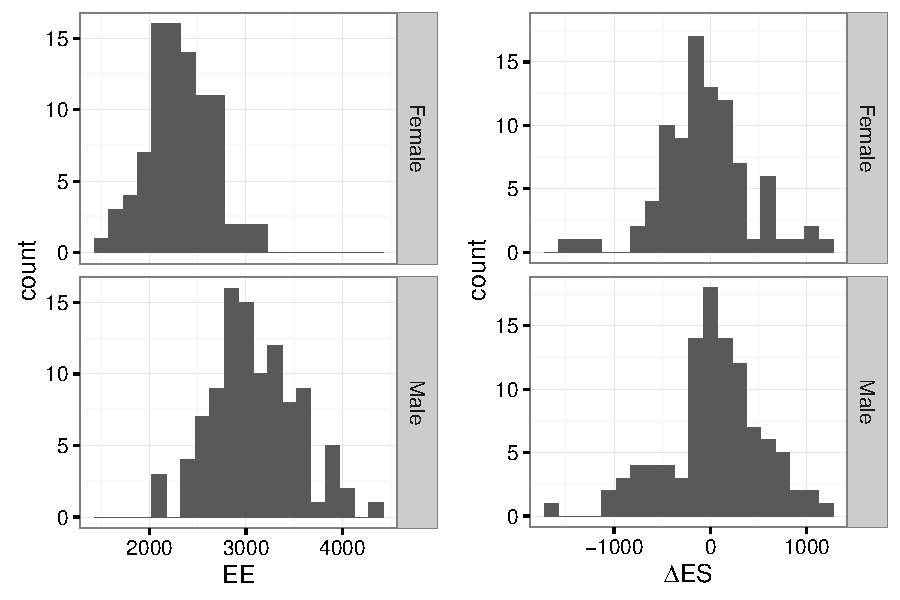
\includegraphics[width=\maxwidth]{figure/ebsw-1} 

}

\caption[Distribtion of EE (left) measured by DLW and ]{Distribtion of EE (left) measured by DLW and $\Delta$ES measured by DXA (right). Females on top, Males on bottom. Includes data from EBS from individuals who receieved DLW measurements.}\label{fig:ebsw}
\end{figure}


\end{knitrout}




\begin{knitrout}
\definecolor{shadecolor}{rgb}{0.969, 0.969, 0.969}\color{fgcolor}\begin{figure}

{\centering 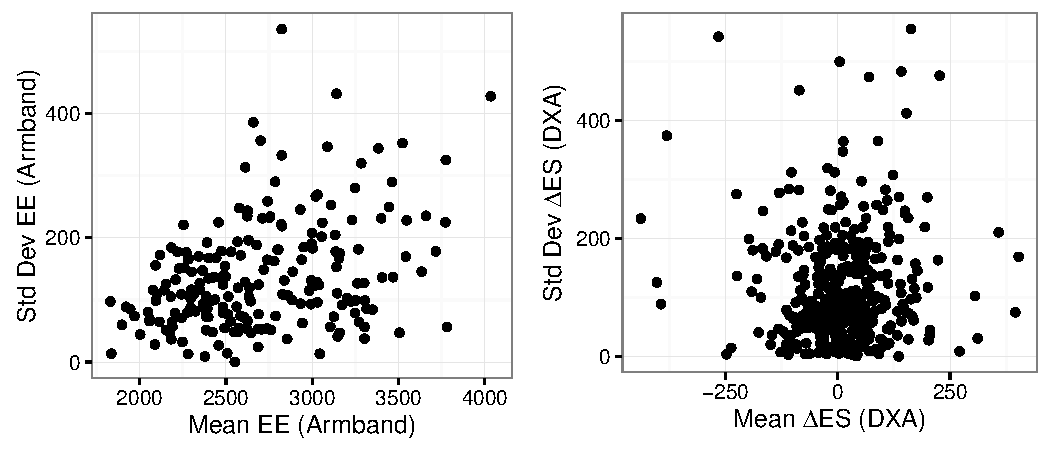
\includegraphics[width=\maxwidth]{figure/ebsdiag-1} 

}

\caption[Variance Diagnostic Plots]{Variance Diagnostic Plots. The left shows the mean EE (Armband) for an individual vs his/her standard deviation of EE based on replicates. The right is the same except for $\Delta$ES measured by DXA.}\label{fig:ebsdiag}
\end{figure}


\end{knitrout}


\begin{knitrout}
\definecolor{shadecolor}{rgb}{0.969, 0.969, 0.969}\color{fgcolor}\begin{figure}

{\centering 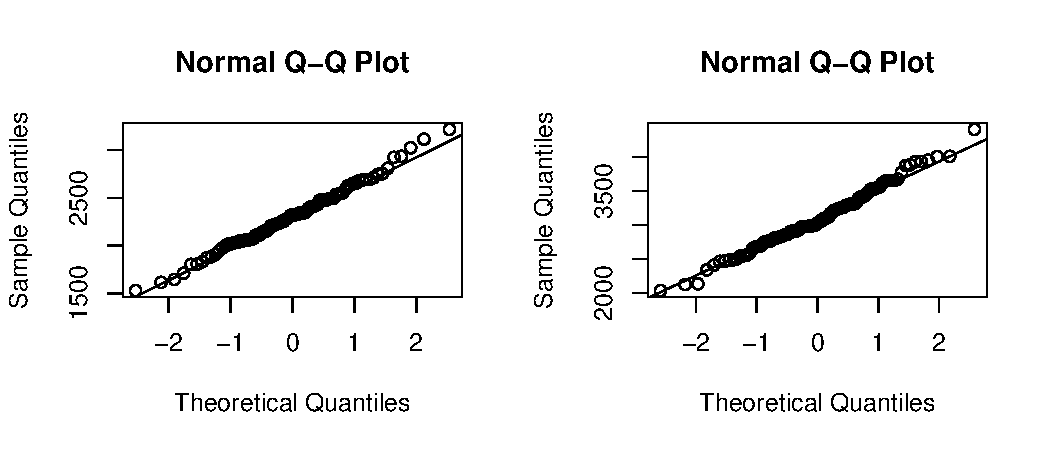
\includegraphics[width=\maxwidth]{figure/ebsdiag2-1} 

}

\caption[Normal Quantile Plots for EE as measured by DLW for Female (left) and Male (right)]{Normal Quantile Plots for EE as measured by DLW for Female (left) and Male (right). Data is from those who recieved DLW in EBS.}\label{fig:ebsdiag2}
\end{figure}


\end{knitrout}

\begin{knitrout}
\definecolor{shadecolor}{rgb}{0.969, 0.969, 0.969}\color{fgcolor}\begin{figure}

{\centering 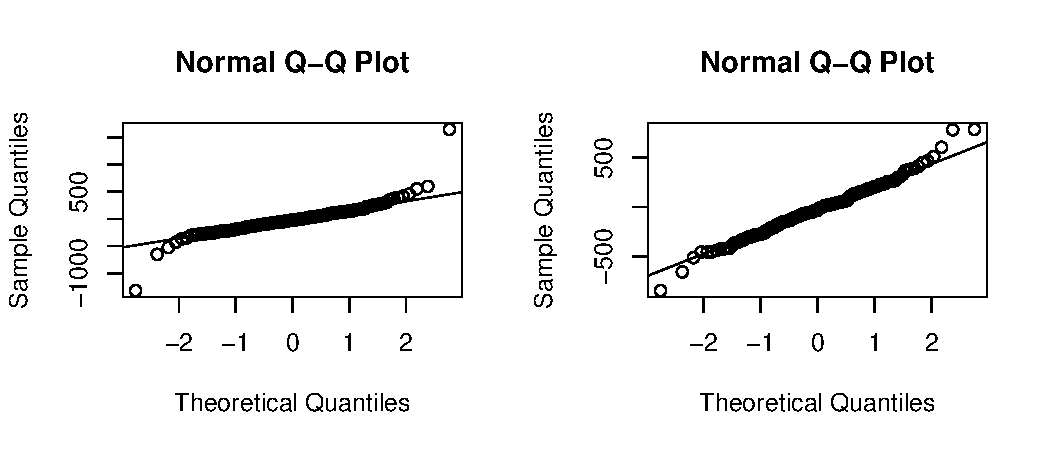
\includegraphics[width=\maxwidth]{figure/ebsdiag3-1} 

}

\caption[Normal Quantile Plots for differenced ]{Normal Quantile Plots for differenced $\Delta$ES ((12m DXA - 9m DXA)-(9m DXA - 6m DXA)) as measured by DXA for Female (left) and Male (right). Data is from those who had DXA scans at 6,9,12 months}\label{fig:ebsdiag3}
\end{figure}


\end{knitrout}


\begin{knitrout}
\definecolor{shadecolor}{rgb}{0.969, 0.969, 0.969}\color{fgcolor}\begin{figure}

{\centering 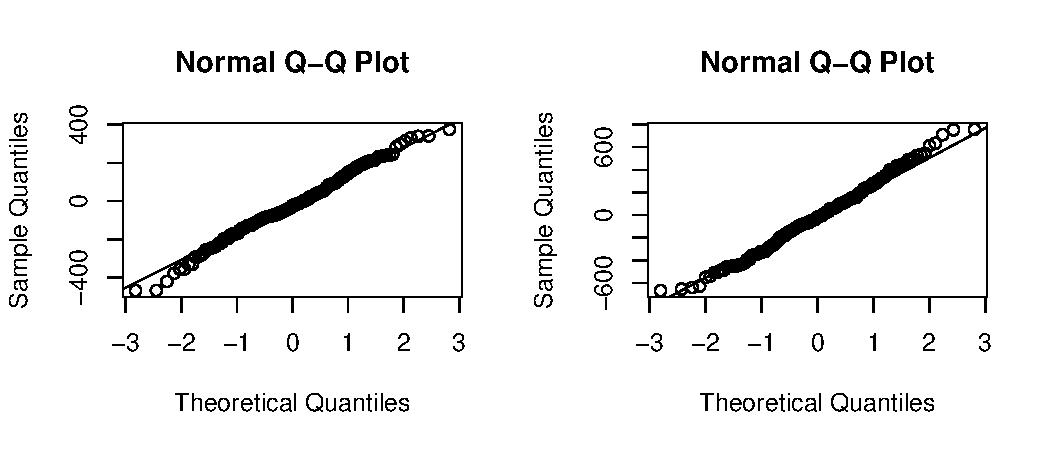
\includegraphics[width=\maxwidth]{figure/ebsdiag4-1} 

}

\caption[Normal Quantile Plots for differenced EE (12m EE - 9m EE) as measured by armbands for Female (left) and Male (right)]{Normal Quantile Plots for differenced EE (12m EE - 9m EE) as measured by armbands for Female (left) and Male (right). Based on entire EBS individuals who remained for entire 12 months}\label{fig:ebsdiag4}
\end{figure}


\end{knitrout}








\begin{kframe}


{\ttfamily\noindent\bfseries\color{errorcolor}{\#\# Error in eval(expr, envir, enclos): could not find function "{}stargazer"{}}}\end{kframe}


%----------------------------------------------------%
%------------------%
%\section{Data Structure}
%------------------%
%----------------------------------------------------%
%------------------%
\section{Simulated Data}
%------------------%

In this section we describe how we simulate a data set that reflects our problem. Our simulated data needs to be sufficiently complex and incorporate dependence in order to represent the distributions of true EE and EI, as well as gold standard measurements and cheap measurements. We need to simulate data for all the components in \eqref{fullmodel} as well as the latent variables ($X_i^{EE}, X_i^{\Delta ES}$). We will explore measurement errors for the gold standard and cheap measurements in 3 different situations: normal errors, skewed errors, bimodal errors. 

%-------------------------%
\subsection{Demographic Covariates}
%------------------------------

For this simulation, we used three covariates: gender, age, BMI. Using a total sample size of 300, we sampled 300 Bernoulli(0.5) to determine gender. Age was determined as a Uniform(20,40). The age range was chosen because the Energy Balance Study \cite{hand}, which has related data used this age range, so it will be easier to compare real data with this simulated data. BMI for an individual was simulated from a Normal(27,5) since the average BMI for an American is around 27 \cite{cdc}. All these values were simulated independently. Let $Z$ be the matrix of dimension 300$\times$3 with all covariate values.


%------------------------------
\subsection{Latent Variables}
%------------------------------

We simulate ($X_i^{EE}, X_i^{EI}$) from a mixture of 5 bivariate t-distributions. 60 observation pairs will be simulated from 5 different bivariate t's each. Simulation was done using the \texttt{rmvt} function in the \texttt{mvtnorm} package in \texttt{R}. The mean of the 2-dimensional vector for each of the 5 t-distributions will be a constant plus a linear combination of the covariates described above. The scale matrix for each of the 5 t-distributions will consist of constants for standard deviations and correlation chosen empirically. The degrees of freedom will remain equal to 5 throughout. 

% this should be for within person variability
% The standard deviation of EE will always be slightly lower than the standard deviation of EI for the same component. This is a realistic assumption as the amount one consumes typcially varies more than one exercises. 

We let the correlation between EE and EI be the same for every component of the mixture. This value was determined empirically through the EBS data. Table \eqref{xparams} shows the values of the mean and standard deviation for EE and EI for every component. The coefficients for the covariates will remain constant across components. The values used for the vector $\gamma_{ee}=(300,14,-7)$ and $\gamma_{es}=(-200,8,-5)$ for gender, BMI and age, respectively. $Z_{comp,k}$ is a 60x3 matrix of covariate values corresponding to the 60 individuals in component $k$.  Once 300 data pairs ($X_i^{EE}, X_i^{EI}$) are simulated according to this procedure, we can then calculate  $X_i^{\Delta ES}$ using the energy balance equation. Figure \ref{fig:latentx} shows histograms for the latent variables for one simulated data set. Figure \ref{fig:contourx} gives contours of the bivariate distributions.


\begin{knitrout}
\definecolor{shadecolor}{rgb}{0.969, 0.969, 0.969}\color{fgcolor}\begin{figure}
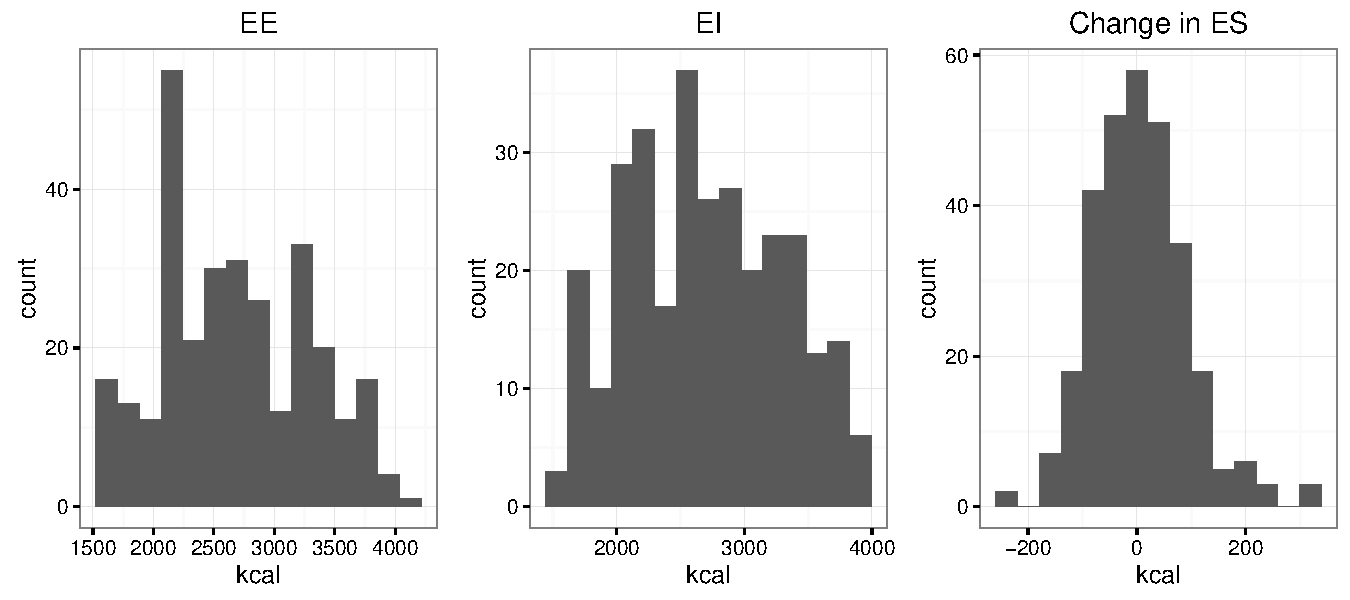
\includegraphics[width=\maxwidth]{figure/latentx-1} \caption[Distribution of simulated latent variables X from one simulated data set]{Distribution of simulated latent variables X from one simulated data set}\label{fig:latentx}
\end{figure}


\end{knitrout}


\begin{knitrout}
\definecolor{shadecolor}{rgb}{0.969, 0.969, 0.969}\color{fgcolor}\begin{figure}
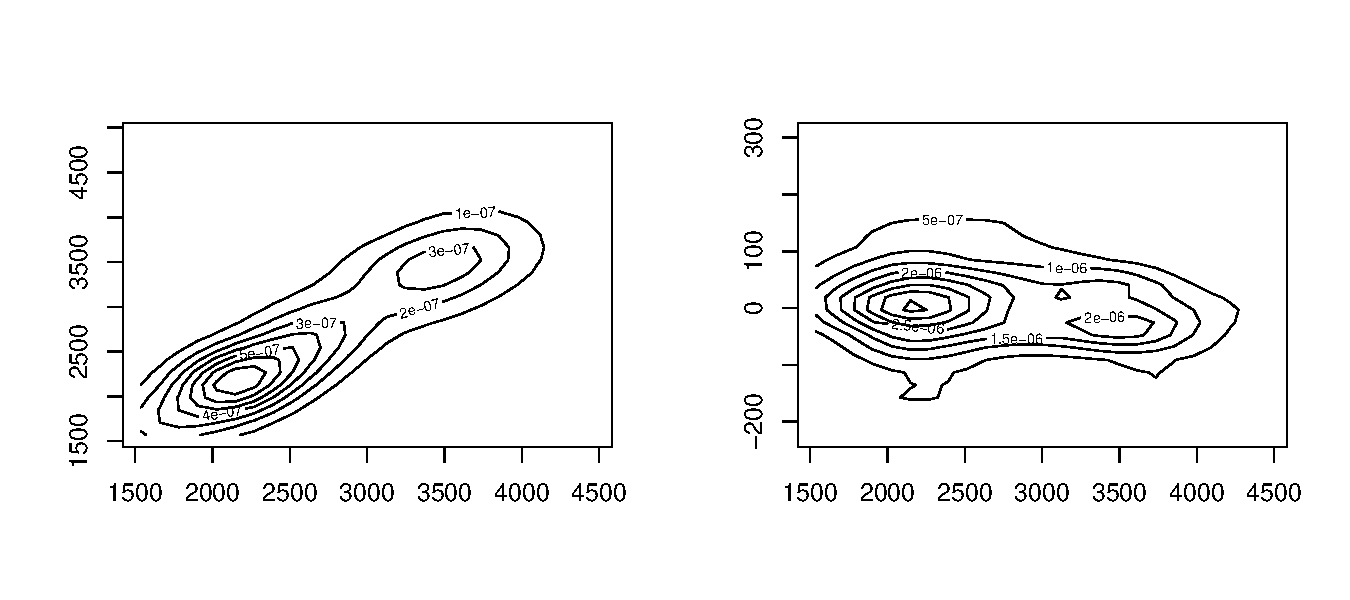
\includegraphics[width=\maxwidth]{figure/contourx-1} \caption[Contour plot os bivariate distributions of one simulated data set for latent variables]{Contour plot os bivariate distributions of one simulated data set for latent variables. $X^{EE}$ vs $X^{EI}$ on left and $X^{EE}$ vs $X^{\Delta ES}$ on right}\label{fig:contourx}
\end{figure}


\end{knitrout}

%%%%%%%%%%%%%%%%%%%%%%%%%%%
%add a contour plot of simulated xes, xee?
%%%%%%%%%%%%%%%%%%%%%%%%%%

\begin{table}
  \begin{tabular}{l|lllll}
    \hline
    & Mean EE & Mean EI & Std Dev EE & Std Dev EI & Cor(EE,EI) \\
    \hline
    Component 1 & 1500 + $\gamma_{ee} Z_{comp,1}$ & 1590 + $\gamma_{ei} Z_1$ & 50 & 70 & 0.4376\\
    Component 2 & 2000 + $\gamma_{ee} Z_{comp,2}$ & 2090 + $\gamma_{ei} Z_2$ & 50 & 65 & 0.4376\\
    Component 3 & 2300 + $\gamma_{ee} Z_{comp,3}$ & 2390 + $\gamma_{ei} Z_3$ & 90 & 120 & 0.4376\\
    Component 4 & 2600 + $\gamma_{ee} Z_{comp,4}$ & 2690 + $\gamma_{ei} Z_4$ & 40 & 50 & 0.4376\\
    Component 5 & 3200 + $\gamma_{ee} Z_{comp,5}$ & 3290 + $\gamma_{ei} Z_5$ & 90 & 120 & 0.4376\\
    \hline
   \end{tabular}
\caption{Mean and Variances for X}
\label{xparams}
\end{table}
 

%-----------------------------
\subsection{Within Person Variability}
%-----------------------------

Recall in \eqref{regressionfcn1}, \eqref{regressionfcn2}, \eqref{gold1}, \eqref{gold2} what the error terms represent: measurement error in the instrument as well as within-person variability (an individual's day to day variation from his \emph{usual}). Again, in terms of \eqref{regressionfcn1}, \eqref{regressionfcn2} this is a working assumption, and here we will correctly put the within person variability within the function. Although we cannot separate the two types of errors when modeling, we can separate them when we simulate data. For the gold standard measurements, let 
\begin{align}
\begin{split}
\label{wpw}
\nu_{ij}^{EE} &= u_{ij}^{EE} + \delta_{ij}^{EE} \\
\nu_{ij}^{\Delta ES} &= u_{ij}^{\Delta ES} + \delta_{ij}^{\Delta ES}
\end{split}
\end{align}

where $u^{EE}$ represents the measurement error in DLW and $u^{\Delta ES}$ represents the measurement error in DXA. $\delta_{ij}^{EE}$ represents the within person variation in EE for person $i$ during time period $j$ from his true mean and  $\delta_{ij}^{\Delta ES}$ similarly represents the within person variation in $\Delta$ES for person $i$ during time period $j$ from his true mean. For the cheap measurements there is a slightly different setup. The within person variability gets added to each individuals \emph{usual} values of EE and $\Delta$ES and thus is affected by the functions $m_{\cdot}(\cdot)$. Therefore we add these within person variation terms $\delta$ to the \emph{usual} values we simulated $X$ to get:

\begin{align}
\begin{split}
\label{wpy}
X_{ij}^{EE} &= X_{i}^{EE} + \delta_{ij}^{EE} \\
X_{ij}^{\Delta ES} &= X_{i}^{\Delta ES} + \delta_{ij}^{\Delta ES}
\end{split}
\end{align} 

where $X_{ij}^{\cdot}$ will be the term in the functions $m_{\cdot}(\cdot)$ to simulate the cheap measurements.

The pairs ($\delta_{ij}^{EE},\delta_{ij}^{\Delta ES}$) will be simulated jointly  but independently across time and individual. We simulate the within person variability terms ($\delta_{ij}^{EE},\delta_{ij}^{\Delta ES}$) according to the bivariate distribution below:


\begin{align}
  \label{delta}
  (\delta_{ij}^{EE}, \delta_{ij}^{\Delta ES}) &\overset{iid}{\sim} N\left(
  \begin{bmatrix}
  0\\
  0
  \end{bmatrix}
  ,
  \begin{bmatrix}
  \sigma_{\delta^{EE}}^2 & \rho_{\delta}\sigma_{\delta^{EE}}\sigma_{\delta^{\Delta ES}} \\
   \rho_{\delta}\sigma_{\delta^{EE}}\sigma_{\delta^{\Delta ES}} & \sigma_{\delta^{\Delta ES}}^2
   \end{bmatrix}
  \right)
\end{align}


  \begin{align}
  \begin{split}
    \label{withinvar5}
  \sigma_{\delta^{EE}} &= 150\\
  \sigma_{\delta^{\Delta ES}} &= 50 \\
  \rho_{\delta} &= -0.266
  \end{split}
  \end{align}


%-----------------------------
\subsection{Gold Standard Measurements}
%-----------------------------

We assume DLW and DXA are unbiased measurements of EE and $\Delta$ES, respectively. These measurements are simulated according to \eqref{gold1},\eqref{gold2} where we further broke down $\nu$ in \eqref{wpw}.  The $u$ term represents the measurement error components we still need to specify and $\delta$ represents the within person component of the error which already described how to simulate. We will assume the $u$ terms are independent within and across individuals as well as mutually with all $\delta$ and $X$. 


From these simulated values, we then get simulated gold standard data $W_{ij}^{EE},W_{ij}^{\Delta ES}$ via \eqref{gold1},\eqref{gold2}. We will simulate measurement errors for the gold standard measurements (and cheap measurements) from a total of three different distributions: normal, skewed normal, and mixture of two normals that is bimodal and centered around 0. The specification for the normal errors are given in \eqref{nerror}. The skewed normal distribution was introduced by Fernandez and Steel \cite{fernandez}. The pdf of the skewed normal is the limit of \eqref{snorm} as $\nu$ goes to $\infty$. $\gamma$ is the skewness parameter, for $\gamma >1$, this results in a right skewed distribution and $\gamma <1$, a left skewed distribution. The measurement error for this distribution is specified by \eqref{snerror}. The final distribution for measurement errors which we explore is a bimodal mixture of two normal distributions. We constructed it such that it is symmetric and centered around 0. This distribution is specified by \eqref{bnerror}. Parameters were chosen such that the means of all error distributions are 0, and the variances for each distribution is the same within EE within $\Delta$ES. Values of the standard deviation parameters are given in \eqref{goldvar}. We simulate from the skewed normal distribution using the R package \texttt{fGarch}. Figure \eqref{fig:errordist} shows density plots of all three distributions using our specified standard deviation and skew parameters.  

\begin{multicols}{2}
\noindent 
  \begin{align}
  \begin{split}
  \label{nerror}
  u_{ij}^{EE} &\overset{iid}{\sim} N(0,\sigma_{\nu^{EE}}^2) \\
  u_{ij}^{\Delta ES} &\overset{iid}{\sim} N(0,\sigma_{\nu^{\Delta ES}}^2) \\
  \end{split}
  \end{align}
  \columnbreak
  \begin{align}
  \begin{split}
    \label{snerror}
  u_{ij}^{EE} &\overset{iid}{\sim} SN(0,\sigma_{\nu^{EE}}^2,10) \\
  u_{ij}^{\Delta ES} &\overset{iid}{\sim} SN(0,\sigma_{\nu^{\Delta ES}}^2,10) \\
  \end{split}
  \end{align}
\end{multicols}


\begin{align}
  \begin{split}
  \label{bnerror}
  u_{ij}^{EE} &\overset{iid}{\sim} 0.5\times N(-175,\sigma_{\nu^{EE}}^2-175^2) +
   0.5\times N(175,\sigma_{\nu^{EE}}^2-175^2) \equiv BM(175,\sigma_{\nu^{EE}}^2)\\
  u_{ij}^{\Delta ES} &\overset{iid}{\sim} 0.5\times N(-45,\sigma_{\nu^{\Delta ES}}^2-45^2) +  0.5\times N(45,\sigma_{\nu^{\Delta ES}}^2-45^2) \equiv BM(45,\sigma_{\nu^{\Delta ES}}^2)\\
  \end{split}
\end{align}

  
\begin{align}
  \begin{split}
   \label{goldvar}
   \sigma_{\nu^{EE}} &= 200 \\
   \sigma_{\nu^{\Delta ES}} &= 53
   \end{split}
\end{align}


  % \begin{align}
  % \label{withinvar1}
  % \sigma_{\nu^{EE}} &= 200 \\
  % \sigma_{\nu^{\Delta ES}} &= 53
  % \end{align}

\begin{align}
\begin{split}
\label{snorm}
  p(y|\mu,\sigma,\nu,\gamma) &= \frac{2}{\gamma+\frac{1}{\gamma}} \frac{\Gamma \left( \frac{\nu+1}{2} \right)}{\Gamma\left(\frac{\nu}{2}\right) (\pi\nu)^{1/2}} \sigma^{-1} \times \\
 & \left\{ 1+ \frac{(y-\mu)^2}{\nu\sigma^2} \left( \frac{1}{\gamma^2} I_{[0,\infty)} (y-\mu) + \gamma^2 I_{(\infty,0)} (y-\mu) \right)  \right\}^{-\frac{(\nu+1)}{2}}
 \end{split}
\end{align}

\begin{knitrout}
\definecolor{shadecolor}{rgb}{0.969, 0.969, 0.969}\color{fgcolor}\begin{figure}

{\centering 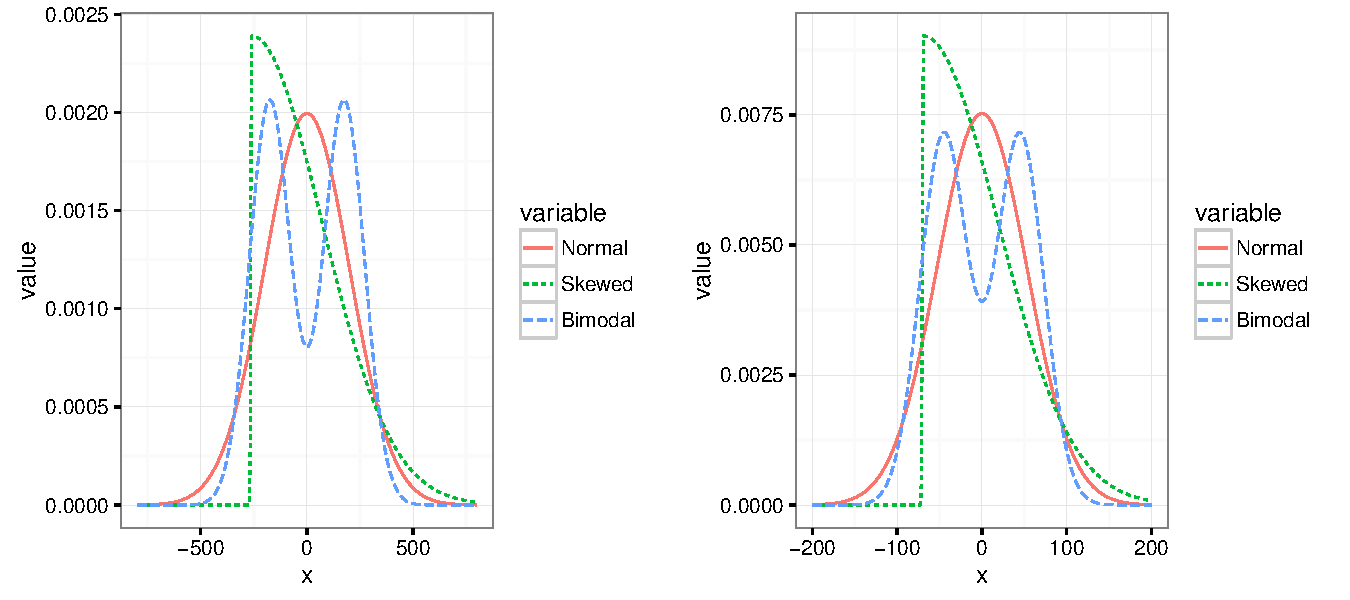
\includegraphics[width=\maxwidth]{figure/errordist-1} 

}

\caption[Measurement Error Distributions, EE on left and ]{Measurement Error Distributions, EE on left and $\Delta$ES on right}\label{fig:errordist}
\end{figure}


\end{knitrout}



%-----------------------------
\subsection{Cheap Measurements}
%-----------------------------

We simulate data for the cheap measurements according to \eqref{regressionfcn1}, \eqref{regressionfcn2}. The error terms in those equations represents measurement error, regression error, and within person variability. Equation \eqref{wpy} shows how we break down the error term from \eqref{regressionfcn1},\eqref{regressionfcn2}. We use the same simulated values  of $\delta$ that we used for the gold standard measurements.

We simulate the measurement error terms $e$ in a similar fashion as the last section. Again we will simulate three different data sets, one with normal errors, one with skewed normal errors, and one with bimodal errors. We assume that the $e$ terms are independent within and across subjects as well as mutually independent with all $\delta$, $X$ and $Z$ terms. We specify these errors similar to the previous section:

\begin{multicols}{2}
\noindent 
  \begin{align}
  \begin{split}
  \label{nerror2}
  e_{ij}^{EE} &\overset{iid}{\sim} N(0,\sigma_{\epsilon^{EE}}^2) \\
  e_{ij}^{\Delta ES} &\overset{iid}{\sim} N(0,\sigma_{\epsilon^{\Delta ES}}^2) \\
  \end{split}
  \end{align}
  \columnbreak
  \begin{align}
  \begin{split}
    \label{snerror2}
  e_{ij}^{EE} &\overset{iid}{\sim} SN(0,\sigma_{\epsilon^{EE}}^2,10) \\
  e_{ij}^{\Delta ES} &\overset{iid}{\sim} SN(0,\sigma_{\epsilon^{\Delta ES}}^2,10) \\
  \end{split}
  \end{align}
\end{multicols}


\begin{align}
  \begin{split}
  \label{bnerror2}
  e_{ij}^{EE} &\overset{iid}{\sim} 0.5\times N(-350,\sigma_{\epsilon^{EE}}^2-350^2) +
   0.5\times N(350,\sigma_{\epsilon^{EE}}^2-350^2) \equiv BM(350,\sigma_{\epsilon^{EE}}^2)\\
  e_{ij}^{\Delta ES} &\overset{iid}{\sim} 0.5\times N(-190,\sigma_{\epsilon^{\Delta ES}}^2-190^2) +  0.5\times N(190,\sigma_{\epsilon^{\Delta ES}}^2-190^2) \equiv BM(190,\sigma_{\epsilon^{\Delta ES}}^2)\\
  \end{split}
\end{align}

  
\begin{align}
  \begin{split}
   \label{cheapvar}
   \sigma_{\epsilon^{EE}} &= 380 \\
   \sigma_{\epsilon^{\Delta ES}} &= 210
   \end{split}
\end{align}

  Different from the gold standard measurements which we assume to be unbiased to the truth, we want to add an element of bias to the cheap measurements. This comes through the functions $m_{ee}$ and $m_{es}$. For this simulated data, we let $m_{ee}(X,Z)$ = $2X_i^{EE}-\frac{4000}{1+e^{-0.002X_i^{EE}-2200}} $ and $m_{es}(X,Z)$ = $\frac{1000}{1+e^{-0.04X_i^{\Delta ES}}} - 2000 + X_i^{\Delta ES}$. These functions represent the bias involved in the cheap instruments as a function of ($X^{EE},X^{\Delta ES}$) and $Z$. Figure \ref{fig:nonlinear} shows $m_{ee}(\cdot)$ on the left and $m_{es}(\cdot)$ on the right both against a  $y=x$ line for comparison. 


\begin{knitrout}
\definecolor{shadecolor}{rgb}{0.969, 0.969, 0.969}\color{fgcolor}\begin{figure}

{\centering 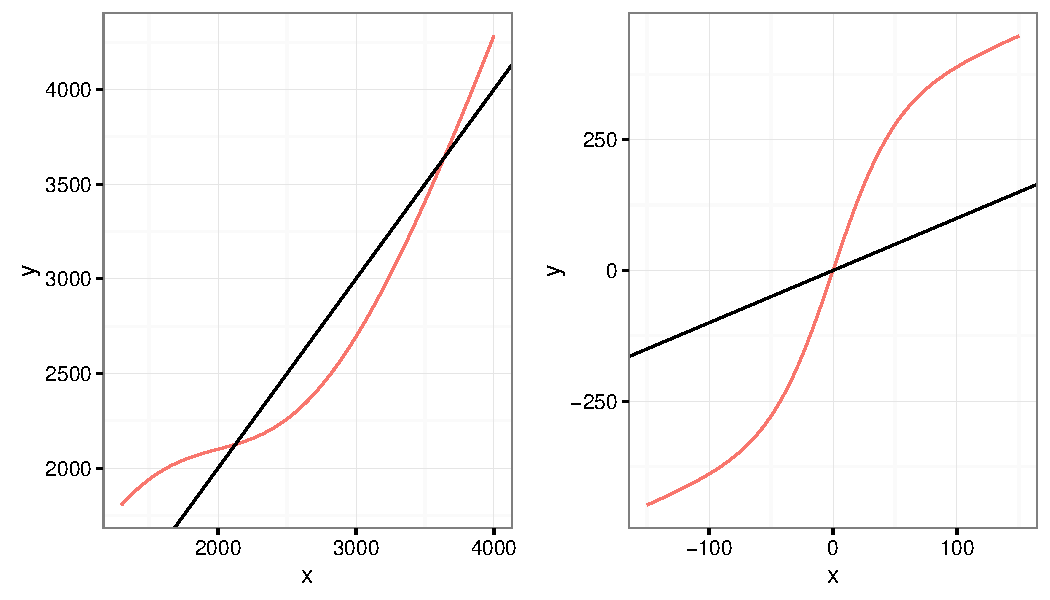
\includegraphics[width=\maxwidth]{figure/nonlinear-1} 

}

\caption[Plot of nonlinear functions ]{Plot of nonlinear functions $m_{ee}()$ (left) and $m_{es}()$ (right), and Y=X is black for reference to unbiased measurement}\label{fig:nonlinear}
\end{figure}


\end{knitrout}



%---------------------------------------------------%
%-------------------%
\section{Estimation}
%-------------------%
%---------------------------------------------------%

We will be taking a Bayesian approach to this problem, and as such, our goal is to estimate the joint  posterior distribution of all parameters and latent variables involved. In our case the posterior is  $p(\boldsymbol{\theta}, X^{EE},X^{\Delta ES}|W^{EE},W^{\Delta ES},Y^{EE},Y^{\Delta ES},Z$). Due to the complexity of our problem and the models we will formulate, we will not be able to analytically derive the posterior distribution. Instead, we will use Markov Chain Monte Carlo (MCMC) methods. For models 0 and 1, we utilized JAGS to simulate draws from the posterior distribution. This was easy to implement and was relatively quick to sample. In order to estimate free knot splines, which allows for dimension change, we must use Reversible Jump MCMC which requires a more complex sampler. We will first present our Gibbs sampler with the reversible jump as a single step, and in the next subsection we will describe the reversible jump in more detail.

\subsection{Gibbs Algorithm}
Here we present our Gibbs algorithm to sample from the joint posterior distribution.

\begin{enumerate}
\item
Set starting values. Let $i=1,...,n$ represent the number of individuals, and $j=1,...,J$ represent the number of replicates for each individual. Assume for simplicity each individual has the same number of replicates.

\item
Set b=0. Run the MCMC below B times. Update tuning parameters $C_{X_i}$, covariance for random walk by setting $C_{X_i} = \frac{2.4^2}{2} \frac{1}{B-1} \sum_{b=1}^{B} (X_i^{EE(b)}-\bar{X}^{EE})(X_i^{\Delta ES(b)}-\bar{X}^{\Delta ES})$. Repeat desired number of times, then throw away draws and continue using new tuning values. 

\item
For iteration k=1,...,K, sample from its full conditional:

\begin{enumerate}
\item
  \{$\zeta_i^{(k)}:i=1,...,n$\} $|$ $\cdot$  
 where P($\zeta_i^{(k)}=h$) = $\frac{\pi_h^{(k-1)} N(\mu_h^{(k-1)},\sigma_h^{2(k-1)})}{\sum_{h=1}^{H}\pi_h^{(k-1)} N(\mu_h^{(k-1)},\sigma_h^{2(k-1)})}$ \\

\item
 \{$V_h^{(k)}:h=1,...,H-1$ \}$|\cdot \overset{ind}{\sim}$  $Beta(1+n_h,\alpha+n_h')$ \\
Set $V_H^{(k)}$ = 1 \\
$n_h = \sum_{i=1}^{n} I(\zeta_i^{(k)}=h)$\\
$n_h' = \sum_{h'=h+1}^{H} n_{h'}$\\


\item
Calculate \{$\pi_i^{(k)}:i=1,...,n$\} $=$ $V_i^{(k)} \prod_{\ell < i} (1-V_{\ell}^{(k)})$


% \item
% $\alpha|\cdot \sim$ $Gamma(a_{\alpha}+n_h+1,b_{\alpha}-\sum_{r=1}^{n_h-1}log(1-V_r))$\\


\item
 \{$\Sigma_{X,h}^{(k)}, h=1,...,H$\} $|\cdot \overset{ind}{\sim}$ $Inv-Wish(d+n_h,\psi+({\bf X_{i,h}^{(k-1)} - \mu_h^{(k-1)}})'({\bf X_{i,h}^{(k-1)} - \mu_h^{(k-1)}}))$ \\

${\bf X_{i,h}} \equiv  {\bf X_i} I(\zeta_i^{(k)}=h)$ \\
${\bf X_i} = (X_i^{EE},X_i^{\Delta ES})$ \\
${\bf \mu_h} = (\mu_{EE,h},\mu_{\Delta ES,h})$



\item
 \{$(\mu_{EE,h}^{(k)},\mu_{\Delta ES,h}^{(k)}), h=1,...,H$ \} $|\cdot \overset{ind}{\sim} N(M_{\mu}',C_{\mu}')$ \\
$C_{\mu}' = (C_{\mu}^{-1} + n_h \Sigma_{X,h}^{-1(k)})^{-1}$ \\
$M_{\mu}' = C_{\mu}'(C_{\mu}^{-1}M + n_h \Sigma_{X,h}^{-1(k)} {\bf \bar{X}^{(k-1)}})$ \\
${\bf \bar{X}} = \frac{1}{n_h}\sum_{i=1}^{n} {\bf X_{i,h}}$ \\

\item
 $\sigma^{2(k)}_{\epsilon^{EE}} |\cdot \sim IG(a_{yee}+J\times \frac{n}{2},b_{yee}+\frac{1}{2}\sum_{i=1}^{n}\sum_{j=1}^{J}(Y_{ij}^{EE}-m_{ee}(X_i^{EE(k-1)};\boldsymbol{\beta_{ee}^{(k-1)}})-\boldsymbol{\gamma_{ee}}^{(k-1)}Z_i)^2)$ \\
 

\item
 $\sigma^{2(k)}_{\epsilon^{\Delta ES}} |\cdot \sim IG(a_{yes}+J\times \frac{n}{2},b_{yes}+\frac{1}{2}\sum_{i=1}^{n}\sum_{j=1}^{J}(Y_{ij}^{\Delta ES}-m_{es}(X_i^{\Delta ES(k-1)};\boldsymbol{\beta_{es}^{(k-1)}})-\boldsymbol{\gamma_{es}}^{(k-1)}Z_i)^2)$ \\
 
 
\item
 $\sigma^{2(k)}_{\nu^{EE}} |\cdot \sim IG(a_{wee}+J\times \frac{n}{2},b_{wee}+\frac{1}{2}\sum_{i=1}^{n}\sum_{j=1}^{J}(W_{ij}^{EE}-X_i^{EE(k-1)})^2)$ \\
 
\item
 $\sigma^{2(k)}_{\nu^{\Delta ES}} |\cdot \sim IG(a_{wes}+J\times \frac{n}{2},b_{wes}+\frac{1}{2}\sum_{i=1}^{n}\sum_{j=1}^{J}(W_{ij}^{\Delta ES}-X_i^{\Delta ES(k-1)})^2)$ \\
 

\item
\{${\bf X_i^{(k)}}:i=1,...,n $\}$|\cdot$ for $i=1,...n$ sample ${\bf X_i^*}$ from $N({\bf X_i^{(k)}},C_{X_i})$ \\

Set ${\bf X_i^{(k)}} = {\bf X_i^*}$ with probability $\alpha_{X_i}$, otherwise set ${\bf X_i^{(k)}} = {\bf X_i^{(k-1)}}$ \\

$\alpha_{X_i} = min\left(1, \frac{f({\bf X_i^*}|\cdot)}{f({\bf X_i^{(k-1)}}|\cdot)}  \right)$ \\

\item
Update ${\boldsymbol{\beta_{ee}},\boldsymbol{\beta_{es}}},k_{ee},k_{es}, {\bf  r_{ee}, r_{es}}$ using RJMCMC described in next section. Calculate $m_{ee}({\bf X^{EE(k)}};\boldsymbol{\beta_{ee}^{(k)}})$ and $m_{es}({\bf X^{\Delta ES(k)}};\boldsymbol{\beta_{es}^{(k)}})$ \\


\item
$\boldsymbol{\gamma_{ee}^{(k)}}|\cdot \sim N(M_{\gamma_{ee}}',C_{\gamma_{ee}}')$ \\
$\boldsymbol{\gamma_{es}^{(k)}}|\cdot \sim N(M_{\gamma_{es}}',C_{\gamma_{es}}')$ \\

$C_{\gamma_{ee}}' = \left( \frac{1}{\sigma^{2(k)}_{\epsilon^{EE}}} Z'Z + \frac{1}{C_{\gamma_{ee}}} I_{3 \times 3} \right)^{-1} $\\
$M_{\gamma_{ee}}' = C_{\gamma_{ee}}' \left( \frac{1}{\sigma^{2(k)}_{\epsilon^{EE}}} Z'({\bf \bar{Y_i}^{EE}} - m_{ee}({\bf X^{EE(k)}};\boldsymbol{\beta_{ee}^{(k)}})) + \frac{m_{\gamma_{ee}}}{C_{\gamma_{ee}} } \right)$ \\

$C_{\gamma_{es}}' = \left( \frac{1}{\sigma^{2(k)}_{\epsilon^{\Delta ES}}} Z'Z + \frac{1}{C_{\gamma_{es}}} I_{3 \times 3} \right)^{-1} $\\
$M_{\gamma_{es}}' = C_{\gamma_{es}}' \left( \frac{1}{\sigma^{2(k)}_{\epsilon^{\Delta ES}}} Z'({\bf \bar{Y_i}^{\Delta ES}} - m_{es}({\bf X^{\Delta ES(k)}};\boldsymbol{\beta_{es}^{(k)}})) + \frac{m_{\gamma_{es}}}{C_{\gamma_{ee}} } \right)$ \\

${\bf \bar{Y_i}^{EE}} = \frac{1}{J} \sum_{j=1}^{J} Y_{ij}^{EE}$ \\
${\bf \bar{Y_i}^{\Delta ES}} = \frac{1}{J} \sum_{j=1}^{J} Y_{ij}^{\Delta ES}$ \\

There are identity matricies because we are assuming independent priors for the linear regression components. 
\end{enumerate}

\end{enumerate}



\subsection{Reversible Jump MCMC}
In order to complete our Gibbs algorithm in the previous section, we need to describe how we estimate the parameters of the free knot spline using RJMCMC. We first present background on estimating free knot splines using RJMCMC. At the end of the section, we present the missing piece in the above algorithm that explains how we sample ${\boldsymbol{\beta_{ee}},\boldsymbol{\beta_{es}}},k_{ee},k_{es}, {\bf  r_{ee}, r_{es}}$. 

RJMCMC was introduced by Green \cite{green} as a way to jump between parameter spaces having different dimensions. It was developed as a Bayesian approach  for model determination. Model selection and model averaging can be implemented straightfoward through the use of this sampler. Although we are not using RJMCMC for the usual type of model selection \emph{per se}, we are using it to select one piece of our model; that is the spline component of our regression. As discussed earlier, we need to specify the position and number of knots for our spline, but since we have no reasonable guess as to what the error free values would look like, we want to account for that uncertainty by treating the position and number of knots as random variables. RJMCMC is the tool that allows us to do this in a Bayesian framework via free knot splines. 

There have been a number of different approaches to Bayesian estimation of free knot splines using RJMCMC \cite{dimatteo},\cite{lindstrom},\cite{johnson}. We will, for the most part, take the approach of Denison et al. \cite{denison}. The approach of Denison et al. is a simple and quick implementation that performs comparably  to the fully Bayesian approach of DiMatteo et al. \cite{dimatteo} for smooth and not highly complex functions when an appropriate adjustment is made (that was pointed out in DiMatteo et al). This is okay for us since we do not expect the function to be highly complex, and this will be shown through our choice of prior for the number of knots for the splines.

Consider the situation where we are interested in estimating a regression spline in the following setup
\begin{align}
\begin{split}
\label{simplespline}
y_i &= f(x_i;\boldsymbol{\beta}) + \epsilon_i \\
\epsilon_i &\overset{iid}{\sim} N(0,\sigma^2)
\end{split}
\end{align}

where the $y_i,i=1,...n$ are the response variable and $x_i,i=1,...n$ is the covariate. We do not want to specify the number or location of the knots. Under the specifications of Denison et al., in RJMCMC for free knot splines there are three possible transitions: 
\begin{enumerate}
\item
Birth of a knot 
\item
Death of a knot
\item
Movement of a knot
\end{enumerate}
where in either of the first two transitions the dimension is changing. Which transition that is proposed depends upon the prior for the number of knots $k$. Using the notation of Denison et al., let the prior probability for $k$ knots be $p(k)$. Then the probability of attempting a birth step, death step or move step are $b_k,d_k,\eta_k$, respectively, where $\eta_k=1-b_k-d_k$, and

\begin{align}
\begin{split}
\label{knotproposal}
b_k &= c \times min\left(1, \frac{p(k+1)}{p(k)} \right) \\
d_k &= c \times min\left(1, \frac{p(k)}{p(k+1)} \right) 
\end{split}
\end{align}

where $0\leq c \leq 1/2$ to ensure $b_k+d_k \leq 1$. If the birth step transition is chosen, a new knot is proposed from the set of available new knots. Denison et al. puts a discrete uniform prior on knot locations so that only observed locations can be knot locations.  A propsed new knot is chosen at random from the set $\mathcal{A}$=\{$x_i,i=1,...n:x_i$ is not currently a knot or within $\ell+1$ locations of a current knot\}. $\ell$ is the order of the splines, so in our case 3 since we're using cubic splines. If the death step transition is chosen, a current knot is picked at random and removed. If the transition step is chosen, a current knot is picked at random and moved to a new location at random from the set $\mathcal{A}$. Once new knots are chosen, construct a spline basis matrix using the observed locations \{$x_i,i=1,...n$\} and the positions of the knots. Then use OLS to estimate the spline parameters $\boldsymbol{\beta}$. Although we could put priors on the spline regression parameters, this adds siginificant computational burden and results have been similar when comparing estimation with OLS versus fully Bayesian \cite{denison}. This is our reason for not having priors on the spline regression parameters in an earlier section. The acceptance probability for each step is of the form given by Green

\begin{align}
\alpha &= min(1, \text{likelihood ratio} \times \text{prior ratio} \times \text{proposal ratio})
\end{align}

Denison et al. gives simplified acceptance probabilities for each of the three transitions under Poisson prior for number of knots and discrete uniform prior for knot locations. In the regression setup in Denison et al., they then sample variance components using a Gibbs step. To check ``convergence" of the chain, Denison et al. suggest monitoring the MSE of the models as defined below. Once the MSE has ``settled down", samples from the posterior should be reasonable.

\begin{align}
MSE &= \frac{1}{n} \sum_{i=1}^{n}(y_i - f(x_i;\boldsymbol{\beta}))^2
\end{align}

%--------------------------------------
\subsection{Our RJMCMC Implementation}
%-------------------------------------

Here we present how we implement our version of RJMCMC for free knot splines. The model \eqref{simplespline} that was used to develop the method in \cite{denison} is simpler than our model in three respects: (i) our covariate value $x_i$ is a latent variable, (ii) we have an additional linear component to our mean function, (iii) the regression model is part of a larger hierarchical model. The third issue doesn't present much of a problem due to our conditional independence assumptions. 

Issue (i) is not as simple. In the free knot spline setup in Denison et al., they have a regression model of the form \eqref{simplespline} where $y$ is the observed response and $x$ is the observed covariate. In our case we do not observe $x$, but rather it is a latent variable that we must sample from using the Gibbs algorithm described in the previous section. Because we have to sample our $x$'s through the Gibbs algorithm, the basis matrix has to be adjusted every iteration. We calculate the basis matrix using the current latent variables and  the proposed knots, if we accept this proposal then the knots, spline coefficients, and thus estimate of $m_{\cdot}(X^{\cdot (k)},\boldsymbol{\beta}_{\cdot}^{(k)})$ are all updated. The bigger problem is what happens when we reject the proposal. Keeping the current knot locations is fine, keeping the current spline regression parameters is fine, but keeping the current predictions doesn't make sense because they are based on $X^{\cdot (k)}$, which is being updated every iteration. What we propose is if we reject the the RJ proposal, we keep the current knots and spline coefficients, calculate a new basis matrix based on the current values of $X^{\cdot (k)}$ and the current knots, then calculate the predicted values by multiplying the basis matrix by the current spline coefficients. An additional complication with $X$ being random instead of fixed has to do with the birth step and the set of available knots to choose from $\mathcal{A}$. We want to pick randomly from the set of $X$ values which we drew in the current iteration of the MCMC, but we do not want a knot to be bigger or smaller than the maximum or minimum value, respectively. This could occur for example, if a new knot is proposed at one of the largest values and it is accepted, then the next iteration through the random walk, the $X$ values could change such that the largest knot is larger than the largest $X$, which causes issues when constructing the basis matrix. To avoid this issue, we exclude the 3 smallest and 3 largest values of $X$ from $\mathcal{A}$.

Our solution to issue (ii) is a simple fix. We fit the free knot spline using the original data $Y^{EE}$ and $Y^{\Delta ES}$ regressed on the B-spline basis matrix generated using the current draw of latent variables $X^{EE}$ and $X^{\Delta ES}$, respectively. Then we calculate $\tilde{Y}^{EE(k)}=Y^{EE}-m_{ee}(X^{EE(k)},\boldsymbol{\beta}_{ee}^{(k)})$ and $\tilde{Y}^{\Delta ES(k)}=Y^{\Delta ES}-m_{es}(X^{\Delta ES(k)},\boldsymbol{\beta}_{es}^{(k)})$ where the superscript $(k)$ represents the $k^{th}$ draw from the MCMC. We then update the $\gamma^{(k)}$ coefficients using $\tilde{Y}^{EE(k)}$ and $\tilde{Y}^{\Delta ES(k)}$ as our data.

This algorithm is run independently for EE and $\Delta$ES regression functions due to conditional independence. Therefore let $(\cdot)$ denote the apppropriate sub/superscript for EE or $\Delta$ES. The reversible jump step that goes into our overall Gibbs algorithm is then:


\begin{enumerate}
\item
Calculate $b_k$ and $d_k$ according to \eqref{knotproposal} \\

\item
Select birth, death, or move step with probabilities $b_k,d_k,1-b_k-d_k$ respectively \\

\item
{\bf Knot Changes} \\
If birth step:\\
%\item
Select a new knot location at random from the set $\mathcal{A}$ and join with current knots $r_{\cdot}^{(k-1)}$ to create the proposed knot locations $r_{\cdot}^{*}$

If death Step:\\
%\item
Sample one knot location from $r_{\cdot}^{(k-1)}$ at random and remove it. 

If move step:\\
%\item
Sample one knot location from $r_{\cdot}^{(k-1)}$ at random, and change it to a new knot location at random from the set $\mathcal{A}$


\item
Calculate the spline basis matrix $B^*_{\cdot}(X^{\cdot(k)})$ using $X^{\cdot(k)}$ and proposed knot locations $r_{\cdot}^{*}$

\item
Calculate proposed spline regression coefficients $\boldsymbol{\beta^*_{\cdot}}$ by using OLS by regressing $Y^{\cdot}$ on $B^*_{\cdot}(X^{\cdot(k)})$

\item
Accept proposed knots and coefficients with probability $\alpha_{\cdot}$ \\

Otherwise set $r_{\cdot}^{(k)}=r_{\cdot}^{(k-1)}$, $\boldsymbol{\beta^{(k)}_{\cdot}} =\boldsymbol{\beta^{(k-1)}_{\cdot}}$ and calculate spline basis matrix $B'_{\cdot}(X^{\cdot(k)})$ using $r_{\cdot}^{(k)}$ in order to calculate mean function $m_{\cdot}(\cdot)$

\begin{align*}
\alpha_{birth} &= min\left(1, \text{Likelihood ratio}\times \frac{n-Z(k)}{n} \right) \\
\alpha_{death} &= min\left(1, \text{Likelihood ratio}\times \frac{n}{n-Z(k)} \right) \\
\alpha_{move} &= min\left(1, \text{Likelihood ratio}\right) 
\end{align*}


\begin{align*}
Z(k) &= 2(\ell+1) + k_{\cdot}(2\ell+1) \\
k_{\cdot} &= length(r_{\cdot}^{(k-1)}) 
\end{align*}


\end{enumerate}

where the acceptance probabilities $\alpha_{rj,\cdot}$ are given in the notation of Denison et al.

%-------------------------------------
%-------------------------------%
\section{Simulation Study}
%-------------------------------%
%-----------------------------------------

In this section we conduct a simulation study to check the performance of the discussed models and modeling assumptions. There are multiple goals for this simulation study. One, the true joint density of $(X_i^{EE},X_i^{\Delta ES})$ must be specified when we model data (or we can assume error free measurements which we'll see is a bad idea), and since this term is never observed by anyone in any study, it is difficult to select a density for. We want to check the robustness of different choices of bivariate densities. Second, the regression functions $m_{ee}$ and $m_{es}$ \eqref{regressionfcn1},\eqref{regressionfcn2} are also unknown, again due to the fact we never observe $(X_i^{EE},X_i^{\Delta ES})$, and therefore don't know the true relationship between $X^{\cdot}$ and the cheap measurements. Third, normal errors  is a common assumption but  can affect predictive performance, and we want to check the robustness to this assumption. We present performance measures such as predicted mean squared error (PMSE) for the regression function in question. Posterior summaries for parameters of interest will be provided as well. 


%---------------------------------------%
\subsection{Setup}
%---------------------------------------%

For this simulation study, we simulated 200 data sets each for normal, skewed, and bimodal errors as described in a previous section. The number of individuals is set to be 300 and the number of replicates is we consider is 2 and 4. Preliminary analysis showed the number of replicates per individual having  more influence than number of individuals. 

Although we'd like to be as flexible as possible with our distributional assumptions on the bivariate latent variables, we also want a model that is stable in its estimates given the data constraints of our application. It would be difficult to get more than 2 replicate measurements on an individual for our gold standard measurements. For 3 replicate measuremnets in the DLW case, this amounts to three 2-week periods along with a washout time in between. In the case of DXA scans, this is 6 scans in a short period of time which can raise flags due to radiation concerns. This is exemplified by the high cost associated with these methods (mainly DLW). Cheap measuremnet tools are not as much of a concern, but they are biased measuremnets of the latent variables unlike the gold standards. During our simulation study, we found that the DP on the latent variables was producing unstable results in parameter estimates and acceptance rates of the random walk Metropolis-Hastings under 2 replicate observations per person. The number of individuals played a much smaller role. Results were stable when 4 replicates per person were used. Results were similar when we used mixtures of normals instead of a DP. This presents an issue in our analysis since it is unrealistic to get that number of replicates in application. Becuase of this issue, we will fit a fourth model using a bivariate normal distribution for the latent variables instead of the Dirichlet Process while still using splines for the regression functions. We refer to this model as BVNS. 

We set the values of the hyperparameters as follows: $M_{\beta_{0,ee}} = M_{\beta_{0,es}} = 0, C_{\beta_{0,ee}} = C_{\beta_{0,es}} = 100000, M_{\beta_{1,ee}} = M_{\beta_{1,es}} = 1, C_{\beta_{1,ee}} = C_{\beta_{1,es}} = 100000, M_{\gamma_{ee}} = M_{\gamma_{es}} = 0, C_{\gamma_{ee}} = C_{\gamma_{es}} = 100000, a_{yee} = a_{yes} = a_{wee} = a_{wes} = b_{yee} = b_{yes} = b_{wee} = b_{wes} = 0.1, \psi = I_{2\times 2}, d = 3, M_{\mu} = (2400,0), C_{\mu} = diag(100000,100000), \lambda_{ee} = \lambda_{es} = 1$.

We ran the MCMC for 12,000 iterations, using the first 2000 as burn in. For all models, we ran 3 chains for 12,000 iterations under three different data sets, and convergence for all models was fast as indicated by trace plots and Gelman-Rubin diagnostics less than 1.04.


%-----------------------------------------%
\subsection{Results}
%-----------------------------------------%


%-----------------------------------------%
\subsection{Closer Look at One Simulated Dataset}
%-----------------------------------------%
 
In this section we provide an example analysis using one of the simulated data sets. This gives an idea of the type of results for an individual data set. We provide posterior quantiles to understand uncertainty in estimates. We also provide posterior predictive assessments for our modeling assumptions.  The posterior predictive distributions of interest are given in \eqref{ypostpred},\eqref{wpostpred},\eqref{xpostpred}. For the measurement error models, we are interested in the posterior predictive distributions for $Y,W,X$ because we are placing distributional assumptions on all of them. The forms for these distributions are given below.
  
\begin{align}
  \label{ypostpred}
  p(Y^*|W,Y,Z) &= \int \int p(Y^*|\theta,X,Z) p(\theta, X|Y,W) d\theta dX \\
  \label{wpostpred}
  p(W^*|W,Y,Z) &= \int \int p(W^*|\theta,X,Z) p(\theta, X|Y,W) d\theta dX \\
  \label{xpostpred}
  p(X^*|W,Y,Z) &= \int \int p(X^*|\theta) p(\theta, X|Y,W) d\theta dX
\end{align}


For these, we are interested in whether our model can capture the true quantiles (min, 0.05, 0.1, 0.25, 0.75, 0.9, 0.95, max) of the bivariate latent vector and for both the cheap and gold standard measurements. To get a distribution of values for our quantiles of interest to compare to the truth, we simulate new data based on MCMC iterations. For example, to calculate distributions for the posterior quantiles for the bivariate latent variable $X$, for each iteration from the MCMC, we  take the sampled values of parameters for the joint distribution of $X$ and simulate a new set of $X$ values, and from that new set of values we calcualte the quantiles of interest. Doing this for many MCMC draws, we get distributions for the quantiles of interest. We then compare these distributions to the truth, and if the truth lies well within the bounds it shows the model accurately captures that feature of the data. If the truth lies outside the bounds, it indicates a lack of fit for that component. Because these distributions for quantiles can have large spreads, we also need to pay attention to their ranges as a check for precision. In this section we will only analyze a single data set with replicates per individual with model BVNS fit. 


%--------------------------------%
%\subsection{Model BVN}
%----------------------------------%
% 
We didn't explicitly introduce Model BVNS before, but it is the same as Model DP except we assume a bivariate normal distribution for the latent variables $(X_i^{EE},X_i^{\Delta ES})$ instead of the Dirichlet Process. For brevity, we will only present results under one dataset with skewed errors. This is a simplifying assumption that we will justify in the next subsection. 

Table  \ref{mbvnswpestimates} give posterior quantiles for this model as well as the truth, when applicable. The asterisk next to the truth for the measurement error with respect to the cheap measurements is to indicate this is a Monte Carlo approximation to the truth. Recall we included within person variation in the functions $m_{\cdot}(\cdot)$, but in our model we use the working assumption that the error term accounts for both within person variability and measurement error. Because we can't directly extract the value from the function, we approximate it by generating 10,000 data sets and removing the mean function from the cheap observations, and then calculating the standard deviation of the residual. We then averaged those standard deviation estimates to get the one reported in the table. All variance components are within the 95\% credible intervals but that for the cheap measurement of $\Delta$ES. All the regression coefficients are in the 95\% credible intervals. These regression coefficients have nice interpretation as they are the linear component of the mean function. $\gamma_{1,ee}$ represents the change in reported EE, all else held equal, for the device user being male. In our example, the truth is 300, which means for two identical people except one male, one female, the cheap measurement tool is biased such that it will record the male as having an EE 300 higher than the female. $\gamma_{2,ee}$ represents the effect of BMI on the device, all else held equal. If BMI increases by 1, then the mean EE reported by the device increases by $\gamma_{2,ee}$. $\gamma_{3,ee}$ represents the effect of age, and the interpretation is similar. Again, we could have included many other/different covariates, and their respective interpretations would be easy as well.

Figure  \ref{wpxdiagbvns} shows plots of posterior predictive assessment for the latent variables skewed errors. Under model BVNS, there is much less flexibility than with the Dirichlet Process. Some of that is seen in this figure, as the minimum EE is not captured and has a large amount of variability. Maximum $\Delta$ES is also only barely covered. Otherwise, these diagnostics look surprisingly good given the truth is clearly non-normal. This result is encouraging since we were concerned about the performance of a single bivariate normal distribution versus the Dirichlet Process for the bivariate latent vector. We constructed the same diagnostic plot where the Dirichlet Process was used and unsuprisingly it looked better in terms of coverage and precision, not by a lot though. However, this was only under 4 replicates because of the issues with 2 replicates described earlier. 

Figure \ref{wpwdiagbvns} show the same plots except for gold standard measurements.  Even under skewed errors, there doesn't seem to be any glaring issues as the truth is captured by the distribution. The only concern would be the amount of variability in the distribution for the minimum and maximum values. Figure \ref{wpydiagbvns} show the same plots except for cheap measurements. The issue here is with capturing the minimum value as recorded by cheap measurement. Otherwise, the remaining plots look good, again even under skewed error terms. This gives some confidence in an amount of robustness to misspecification of measurement error distribution.

Figure \ref{predbvnsx} gives one of the main desired outcomes of this study. This figure plots the fitted spline between the truth and the observed cheap measurement. The plot on the left is for the cheap EE measurement, on the right is for $\Delta$ES. The points plotted are from the individual simulated data where the y value is the mean of the two replicates. The red line is the mean spline function from this data set and we also randomly selected 500 MCMC iteration draws for the spline, and plotted them behind the mean. This is of high interest to us because it shows the relationship between what we observe, and what we are ultimately interested in knowing. To calibrate the cheap measurements, we would use the information from this plot as well as the posteriors for the $\gamma$ coefficients that refer to demographic variables.


%Table \ref{pmse2} gives PMSE for both the EE and $\Delta$ES regression functions under normal, skewed, and bimodal errors. Not only does ignoring the measurement error give bad parameter estimates and posterior predictive checks, but also its prediction is poor. Our model that has splines in its regression function  whose knots can varry iteration to iteration performs much better than just a linear model. 

% \begin{table}[ht]
% \centering
% \begin{tabular}{rrrrrr|r}
%   \hline
%  & 2.5\% & 25\% & 50\% & 75\% & 97.5\% & Truth\\
%   \hline
% $\mu_x^{EE}$ & 2610.19 & 2663.99 & 2691.59 & 2719.67 & 2772.07 \\ 
%   $\mu_x^{\Delta ES}$ & -8.11 & -1.42 & 2.08 & 5.61 & 12.38 \\ 
%   $\sigma_{yee}$ & 381.01 & 396.92 & 405.71 & 414.93 & 435.80 \\ 
%   $\sigma_{yes}$ & 296.81 & 309.75 & 316.87 & 324.23 & 339.56 \\ 
%   $\sigma_{wee}$ & 236.55 & 248.84 & 255.74 & 262.91 & 277.50 & 250\\ 
%   $\sigma_{wes}$ & 64.41 & 67.17 & 68.73 & 70.33 & 73.51 & 72.86\\ 
%   $\sigma_{xee}$ & 637.76 & 673.81 & 694.27 & 715.80 & 759.92 \\ 
%   $\sigma_{xes}$ & 67.03 & 72.23 & 75.17 & 78.12 & 84.09 \\ 
%   $\rho$ & -0.23 & -0.15 & -0.11 & -0.06 & 0.02 \\ 
%   $\gamma_{1,ee}$ & 178.48 & 244.17 & 278.90 & 314.08 & 382.01 & 300\\ 
%   $\gamma_{2,ee}$ & -0.05 & 4.81 & 7.34 & 9.87 & 14.70 & 14\\ 
%   $\gamma_{3,ee}$ & -17.51 & -13.32 & -11.09 & -8.84 & -4.59 & -7\\ 
%   $\gamma_{1,es}$ & -296.12 & -241.05 & -212.36 & -183.20 & -126.47 & -200 \\ 
%   $\gamma_{2,es}$ & 3.02 & 6.97 & 9.05 & 11.17 & 15.32 & 8\\ 
%   $\gamma_{3,es}$ & -10.58 & -6.88 & -4.94 & -3.05 & 0.63 & -5\\ 
%   \hline
% \end{tabular}
% \caption{Parameter estimates for Model BVN for Normal errors with correct specification of within person errors}
% \label{mbvnwpestimates}
% \end{table}


\begin{table}[ht]
\centering
\begin{tabular}{rrrrrr|r}
  \hline
 & 2.5\% & 25\% & 50\% & 75\% & 97.5\% & Truth\\
  \hline
$\mu_x^{EE}$ & 2622.55 & 2675.43 & 2703.64 & 2732.01 & 2786.64 \\ 
  $\mu_x^{\Delta ES}$ & -7.62 & -0.93 & 2.59 & 6.10 & 12.84 \\ 
  $\sigma_{yee}$ & 371.38 & 387.03 & 395.75 & 405.05 & 425.11 & $422^*$ \\ 
  $\sigma_{yes}$ & 291.18 & 303.53 & 310.39 & 317.55 & 331.87 & $344^*$ \\ 
  $\sigma_{wee}$ & 241.21 & 253.60 & 260.49 & 267.51 & 281.58 & 250 \\ 
  $\sigma_{wes}$ & 65.05 & 67.98 & 69.56 & 71.24 & 74.65 & 72.862\\ 
  $\sigma_{xee}$ & 641.81 & 679.00 & 699.07 & 720.28 & 764.17 \\ 
  $\sigma_{xes}$ & 65.68 & 70.97 & 73.92 & 76.89 & 82.68 \\ 
  $\rho$ & -0.28 & -0.20 & -0.15 & -0.11 & -0.02 \\ 
  $\gamma_{1,ee}$ & 150.70 & 216.27 & 251.30 & 285.24 & 352.67 & 300 \\ 
  $\gamma_{2,ee}$ & 0.29 & 5.23 & 7.76 & 10.27 & 15.22 & 14\\ 
  $\gamma_{3,ee}$ & -17.58 & -13.31 & -11.06 & -8.85 & -4.57 & -7 \\ 
  $\gamma_{1,es}$ & -297.09 & -244.54 & -217.35 & -190.06 & -138.10 & -200 \\ 
  $\gamma_{2,es}$ & 2.31 & 6.06 & 8.01 & 9.99 & 13.75 & 8\\ 
  $\gamma_{3,es}$ & -9.18 & -5.74 & -3.93 & -2.15 & 1.27 & -5 \\ 
   \hline
\end{tabular}
\caption{Parameter estimates for Model BVNS for Skewed errors with correct specification of within person errors}
\label{mbvnswpestimates}
\end{table}

% \begin{table}[ht]
% \centering
% \begin{tabular}{rrrrrr|r}
%   \hline
%  & 2.5\% & 25\% & 50\% & 75\% & 97.5\% & Truth \\
%   \hline
% $\mu_x^{EE}$ & 2581.07 & 2634.84 & 2662.65 & 2690.48 & 2743.29 \\ 
%   $\mu_x^{\Delta ES}$ & -14.55 & -7.47 & -3.70 & 0.01 & 6.92 \\ 
%   $\sigma_{yee}$ & 245.77 & 261.27 & 269.43 & 277.84 & 297.13 \\ 
%   $\sigma_{yes}$ & 223.45 & 232.56 & 237.53 & 242.90 & 253.34 \\ 
%   $\sigma_{wee}$ & 176.09 & 186.78 & 192.79 & 199.36 & 213.55 & 250\\ 
%   $\sigma_{wes}$ & 48.83 & 50.96 & 52.15 & 53.36 & 55.79 & 72.862 \\ 
%   $\sigma_{xee}$ & 646.03 & 682.15 & 702.09 & 722.74 & 764.86 \\ 
%   $\sigma_{xes}$ & 79.09 & 84.14 & 86.92 & 89.80 & 95.74 \\ 
%   $\rho$ & -0.06 & 0.02 & 0.06 & 0.10 & 0.18 \\ 
%   $\gamma_{1,ee}$ & 125.13 & 175.72 & 201.12 & 226.66 & 276.14 & 300 \\ 
%   $\gamma_{2,ee}$ & 4.54 & 8.05 & 9.86 & 11.66 & 15.18 & 14\\ 
%   $\gamma_{3,ee}$ & -16.95 & -13.86 & -12.24 & -10.63 & -7.58 & -7 \\ 
%   $\gamma_{1,es}$ & -239.57 & -198.67 & -177.29 & -155.91 & -115.00 & -200 \\ 
%   $\gamma_{2,es}$ & 1.66 & 4.61 & 6.19 & 7.71 & 10.72 & 8\\ 
%   $\gamma_{3,es}$ & -7.02 & -4.31 & -2.90 & -1.49 & 1.20 & -5\\ 
%    \hline
% \end{tabular}
% \caption{Parameter estimates for Model BVN for Bimodal errors with correct specification of within person errors}
% \label{mbvnbwpestimates}
% \end{table}

%  %post pred check for X
 % \begin{figure}
 %  \centering
 %  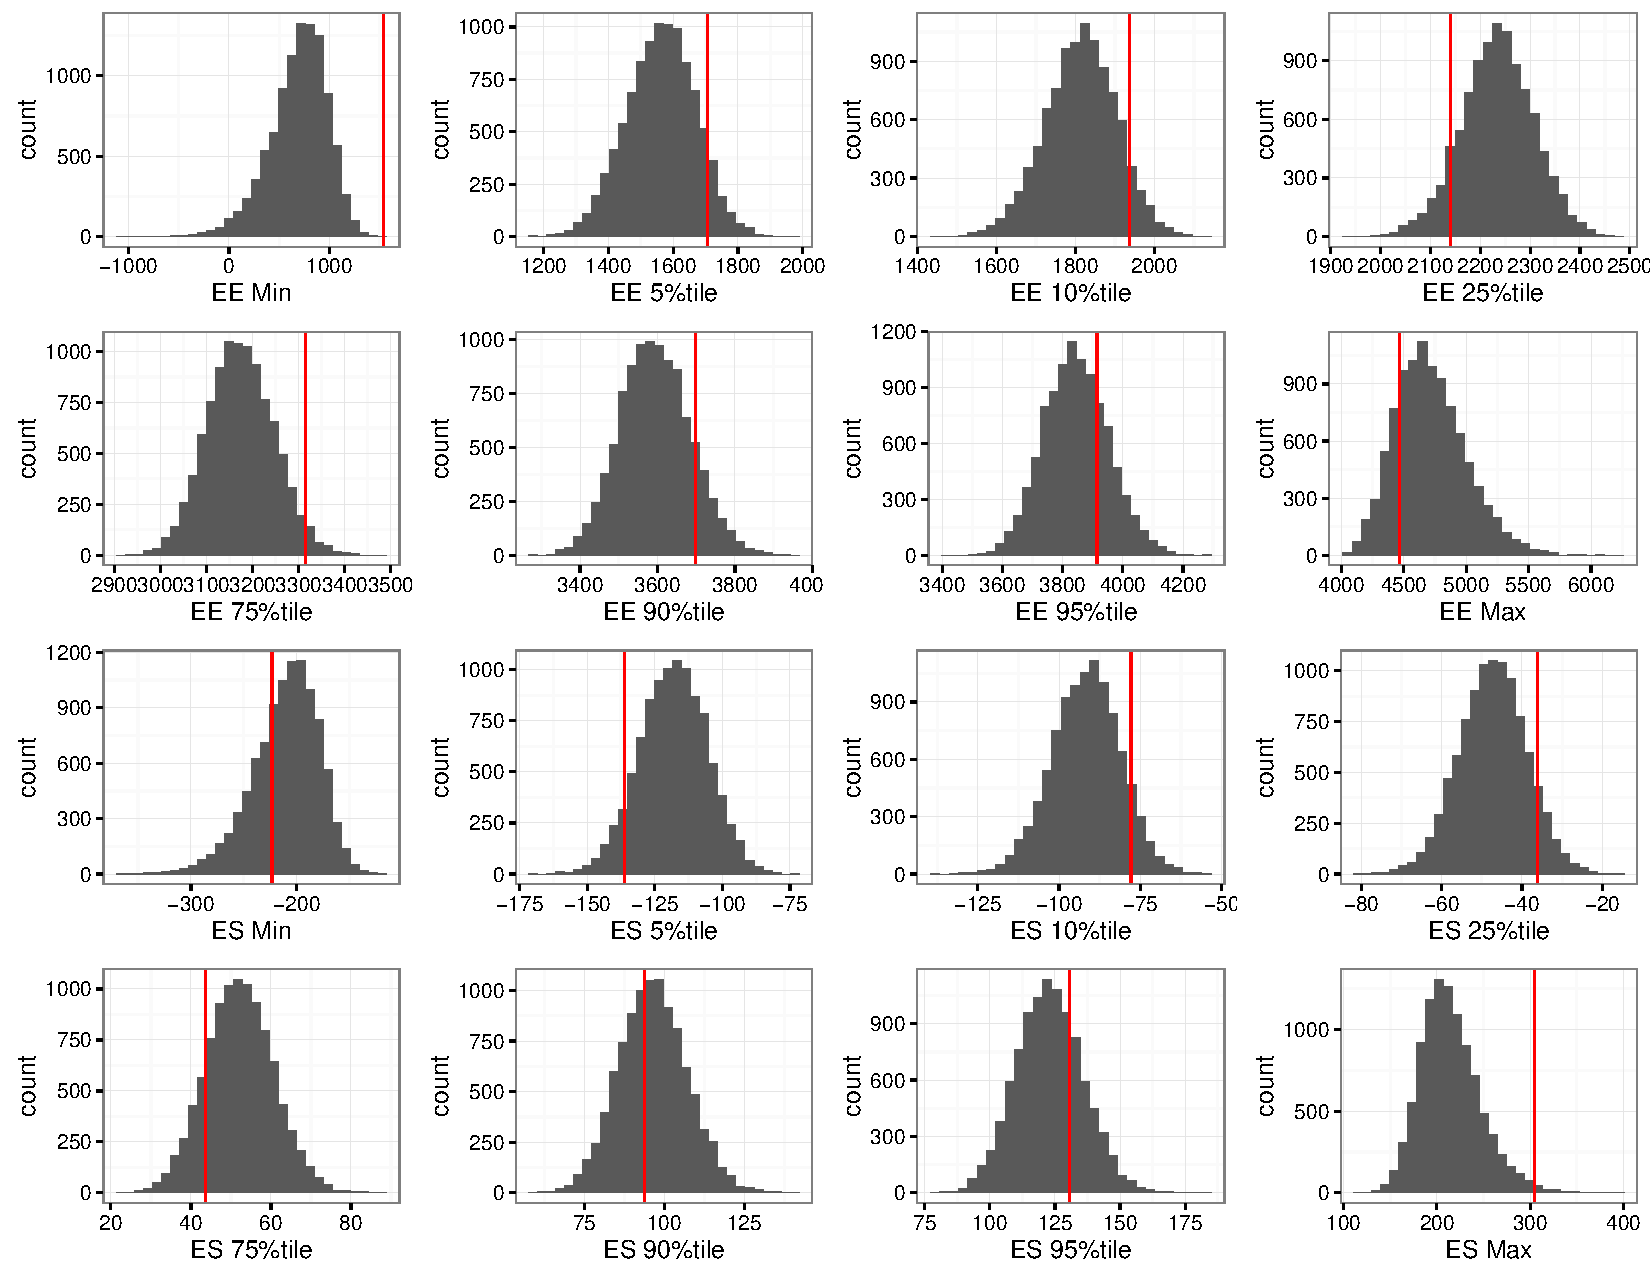
\includegraphics[width=17cm,height=15cm]{manual_figure/wpxdiagbvn.pdf}
 %  \caption{Posterior Predictive Discrepancy Measures For $X^{EE}$ and $X^{\Delta ES}$ for Model BVN with Normal Errors}
 %  \label{wpxdiagbvn}
 %  \end{figure}
 % %post pred check for W
 %  \begin{figure}
 %  \centering
 %  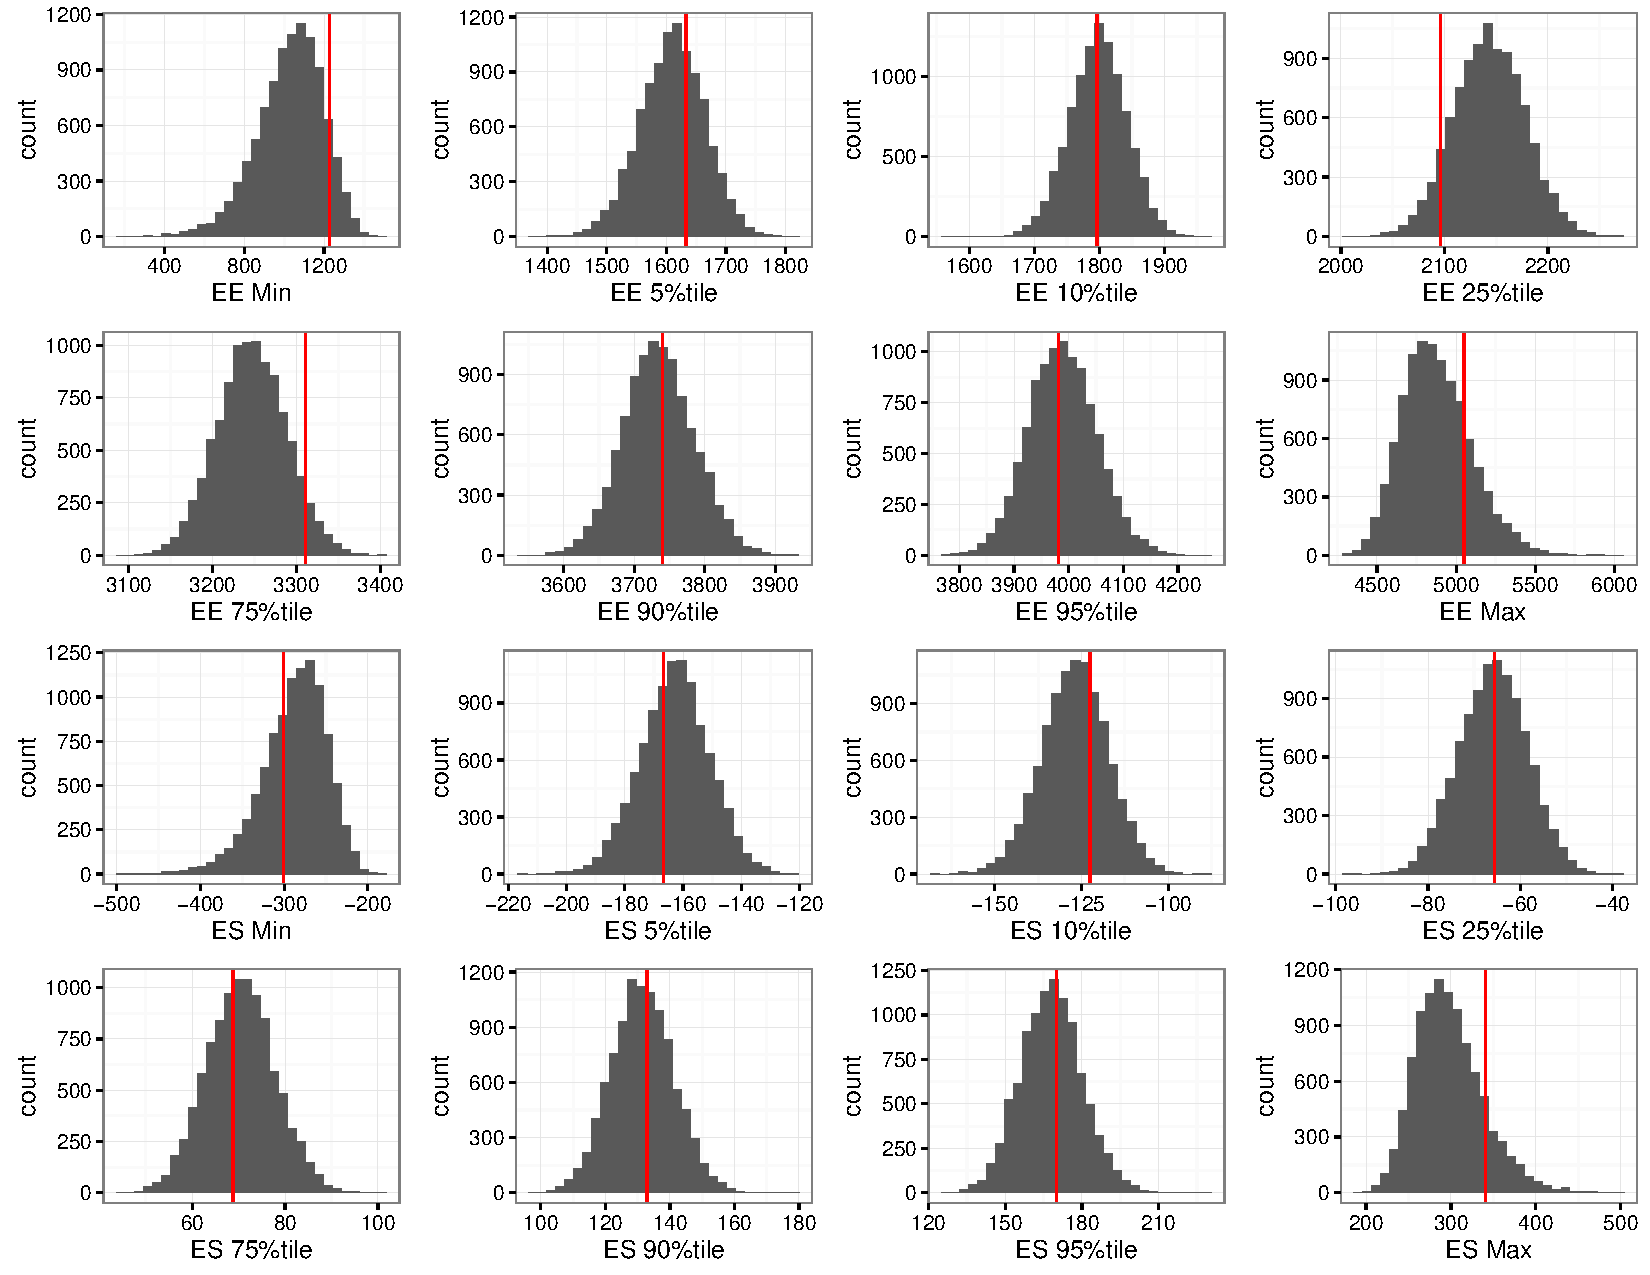
\includegraphics[width=17cm,height=15cm]{manual_figure/wpwdiagbvn.pdf}
 %  \caption{Posterior Predictive Discrepancy Measures For $W^{EE}$ and $W^{\Delta ES}$ for Model BVN with Normal Errors}
 %  \label{wpwdiagbvn}
 %  \end{figure}
 % %post pred check for Y
 %  \begin{figure}
 %  \centering
 %  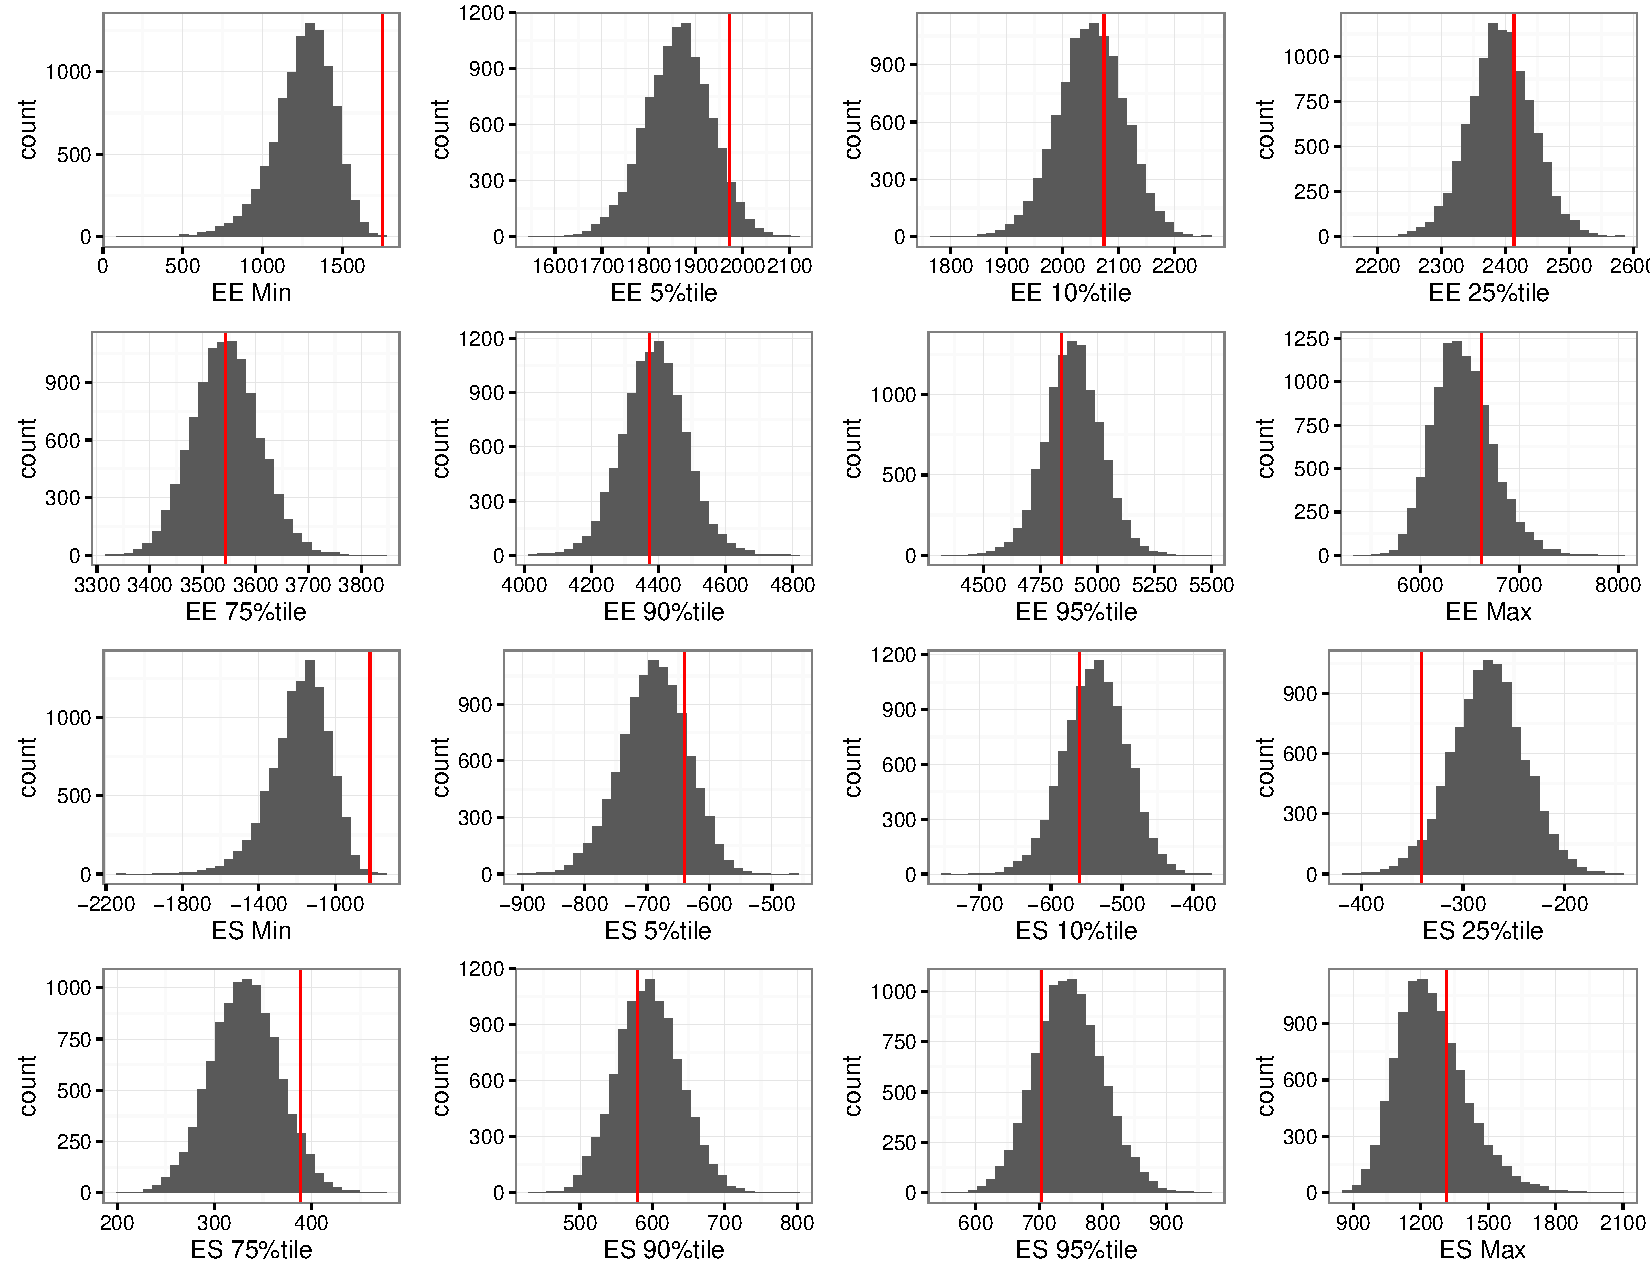
\includegraphics[width=17cm,height=15cm]{manual_figure/wpydiagbvn.pdf}
 %  \caption{Posterior Predictive Discrepancy Measures For $Y^{EE}$ and $Y^{\Delta ES}$ for Model BVN with Normal Errors}
 %  \label{wpydiagbvn}
 %  \end{figure}
% 
% 
%  %post pred check for X
 \begin{figure}
  \centering
  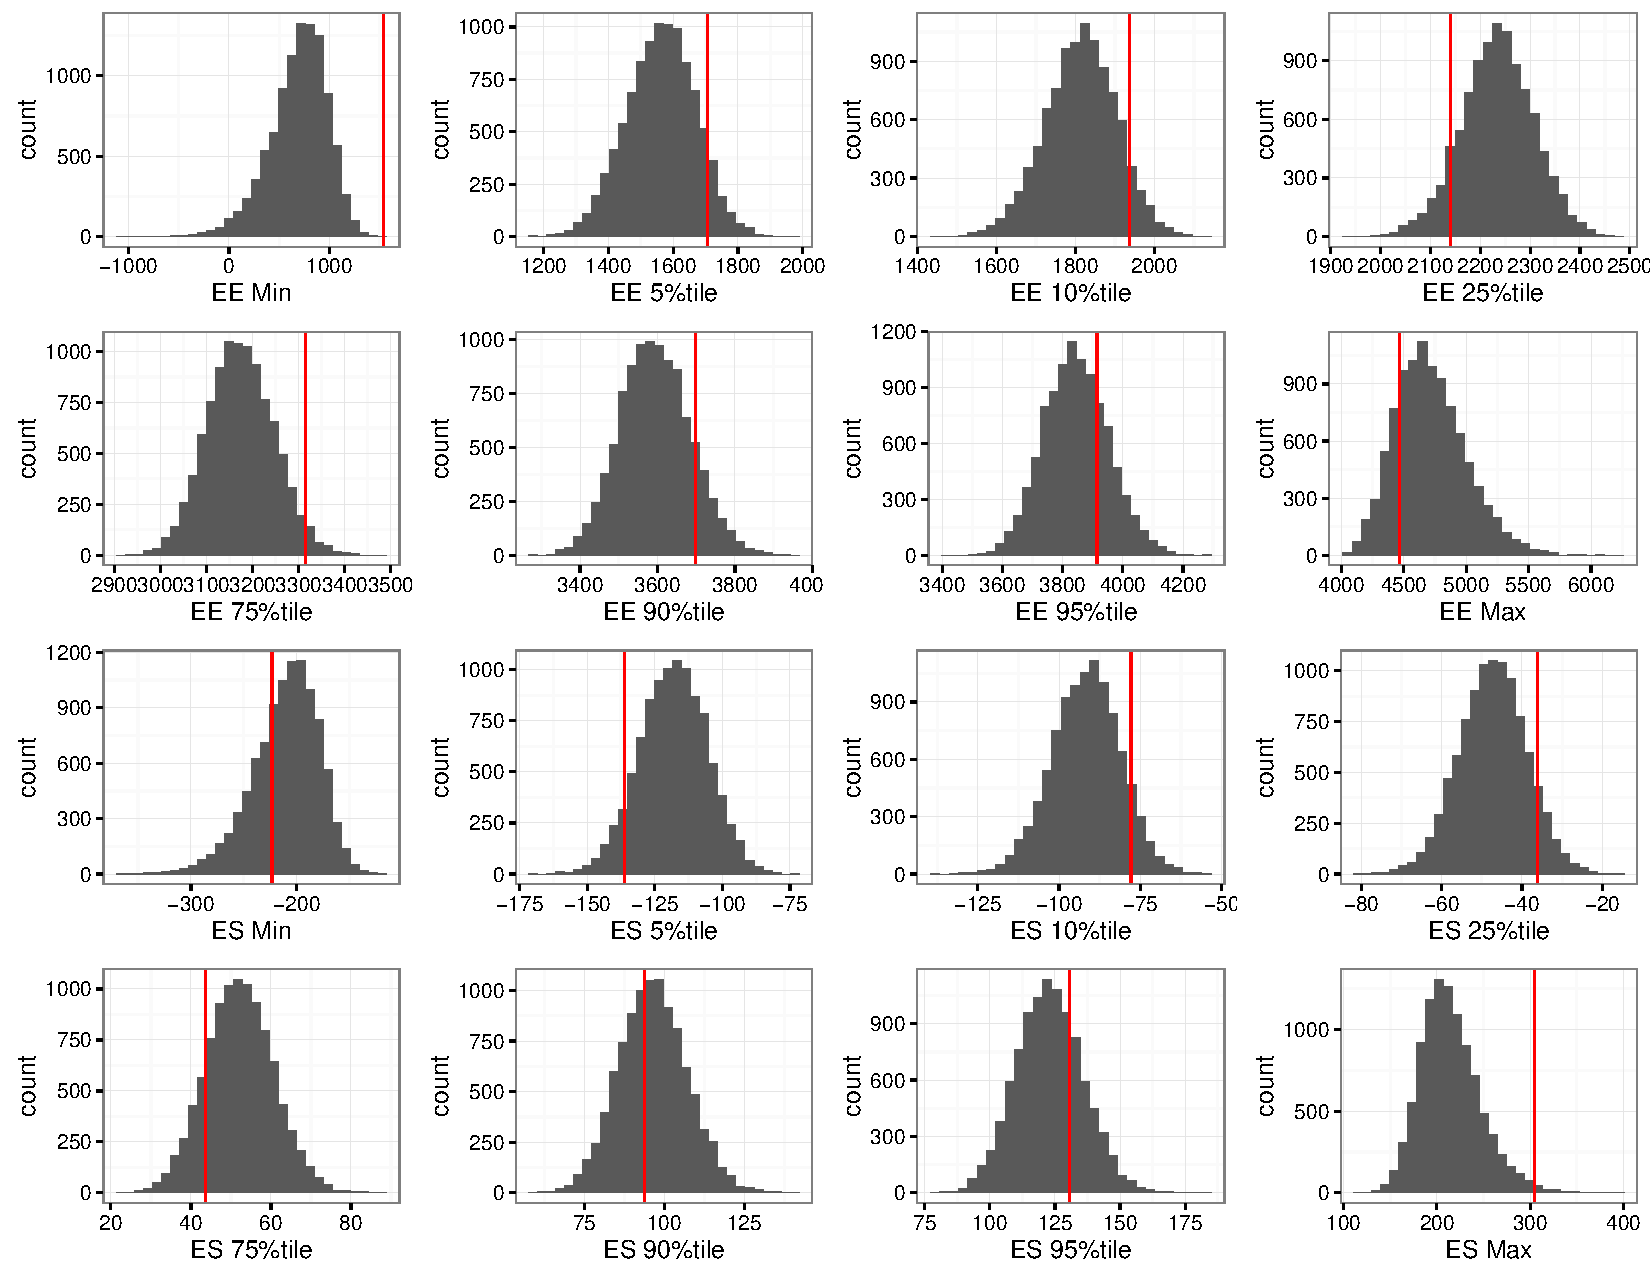
\includegraphics[width=17cm,height=15cm]{manual_figure/wpxdiagbvns.pdf}
  \caption{Posterior Predictive Discrepancy Measures For $X^{EE}$ and $X^{\Delta ES}$ for Model BVNS with Skewed Normal Errors}
  \label{wpxdiagbvns}
  \end{figure}
 %post pred check for W
  \begin{figure}
  \centering
  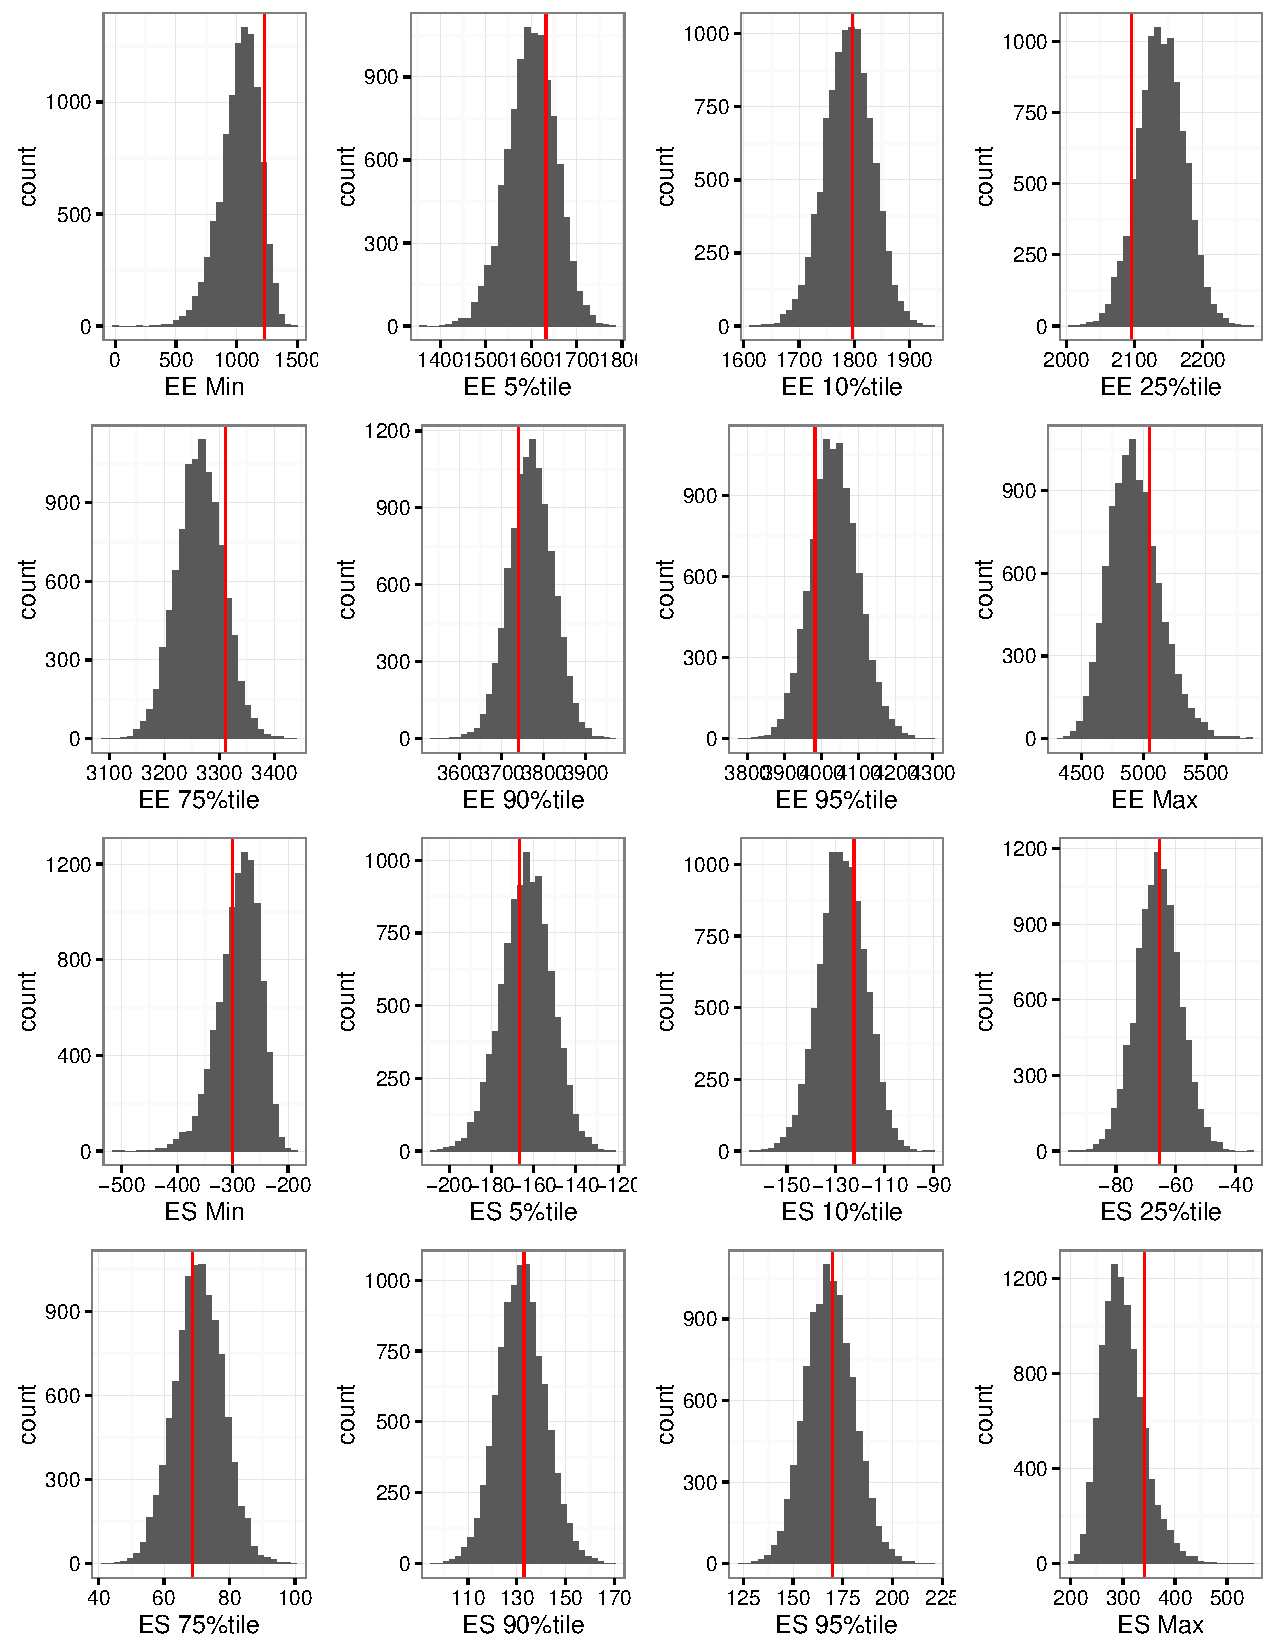
\includegraphics[width=17cm,height=15cm]{manual_figure/wpwdiagbvns.pdf}
  \caption{Posterior Predictive Discrepancy Measures For $W^{EE}$ and $W^{\Delta ES}$ for Model BVNS with Skewed Normal Errors}
  \label{wpwdiagbvns}
  \end{figure}
 %post pred check for Y
  \begin{figure}
  \centering
  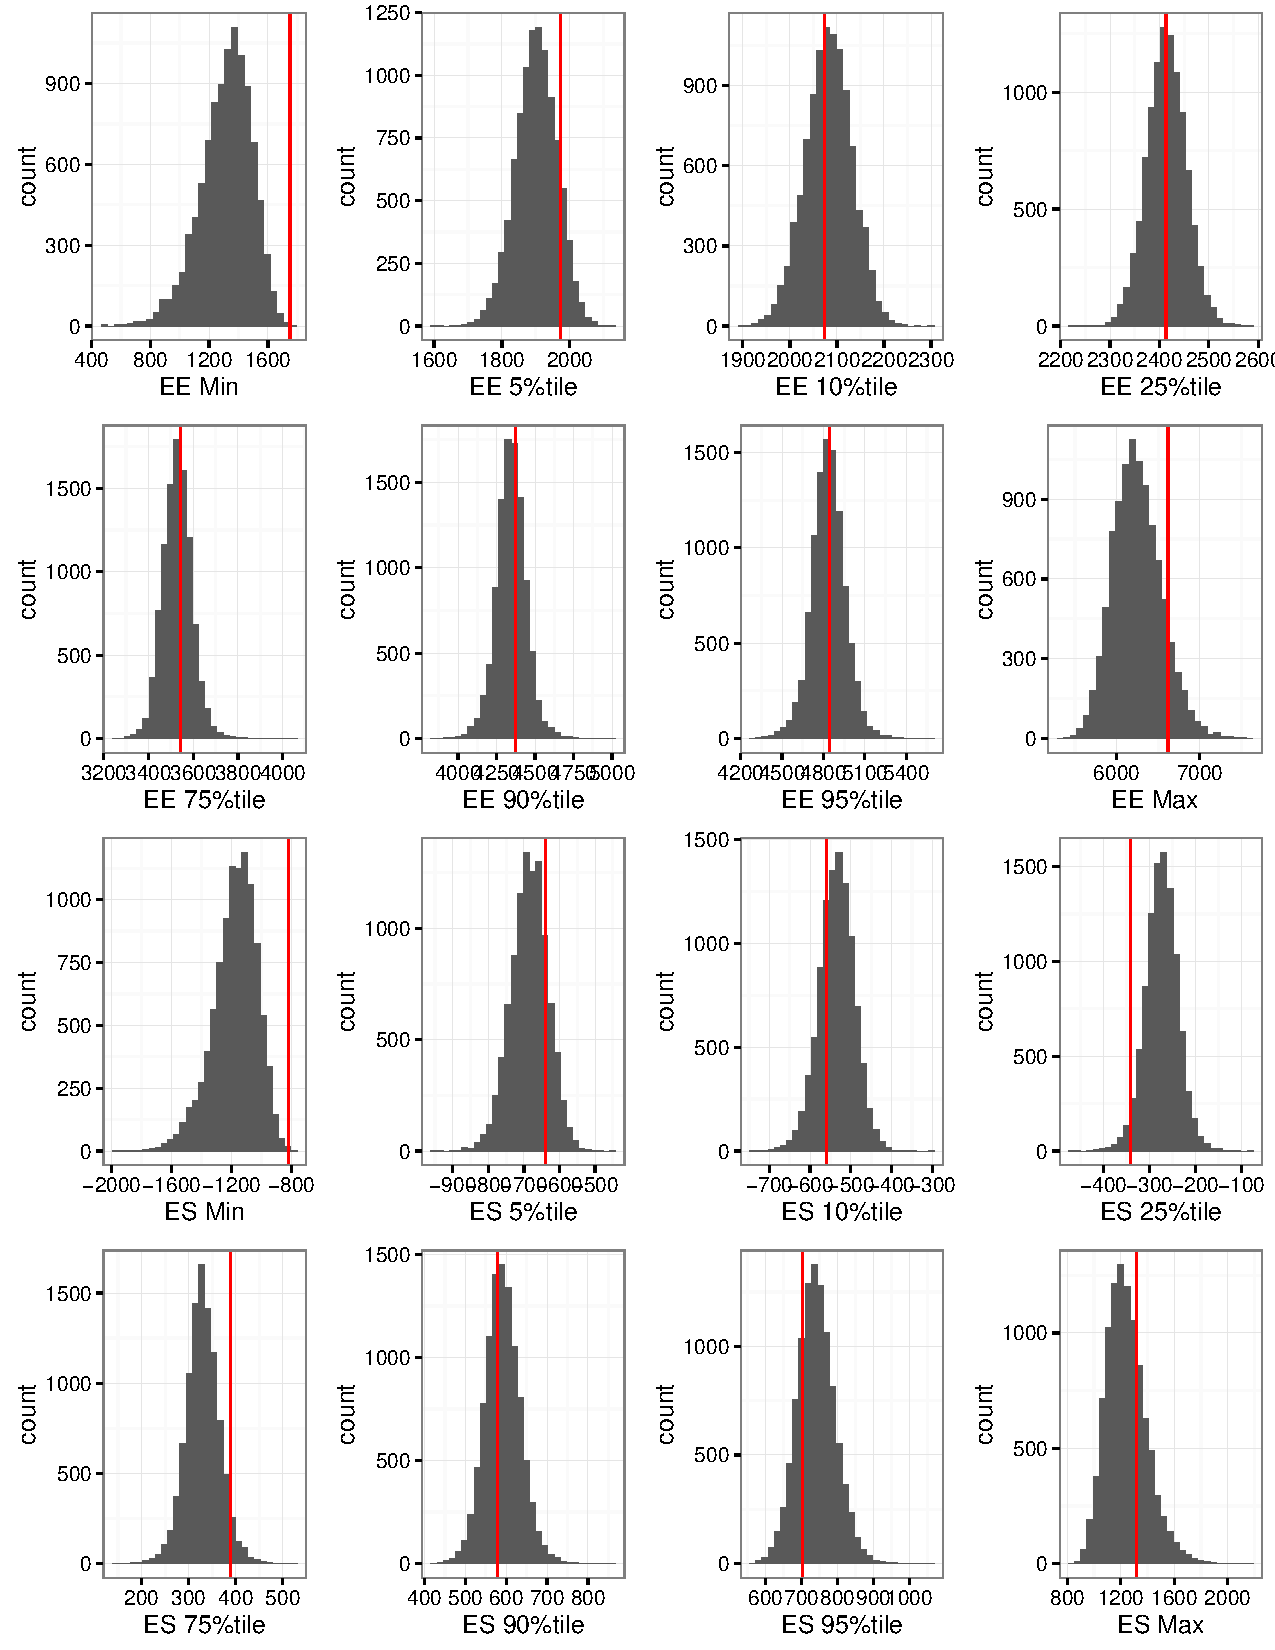
\includegraphics[width=17cm,height=15cm]{manual_figure/wpydiagbvns.pdf}
  \caption{Posterior Predictive Discrepancy Measures For $Y^{EE}$ and $Y^{\Delta ES}$ for Model BVNS with Skewed Normal Errors}
  \label{wpydiagbvns}
  \end{figure}
  
 %   \begin{figure}
 %  \centering
 %  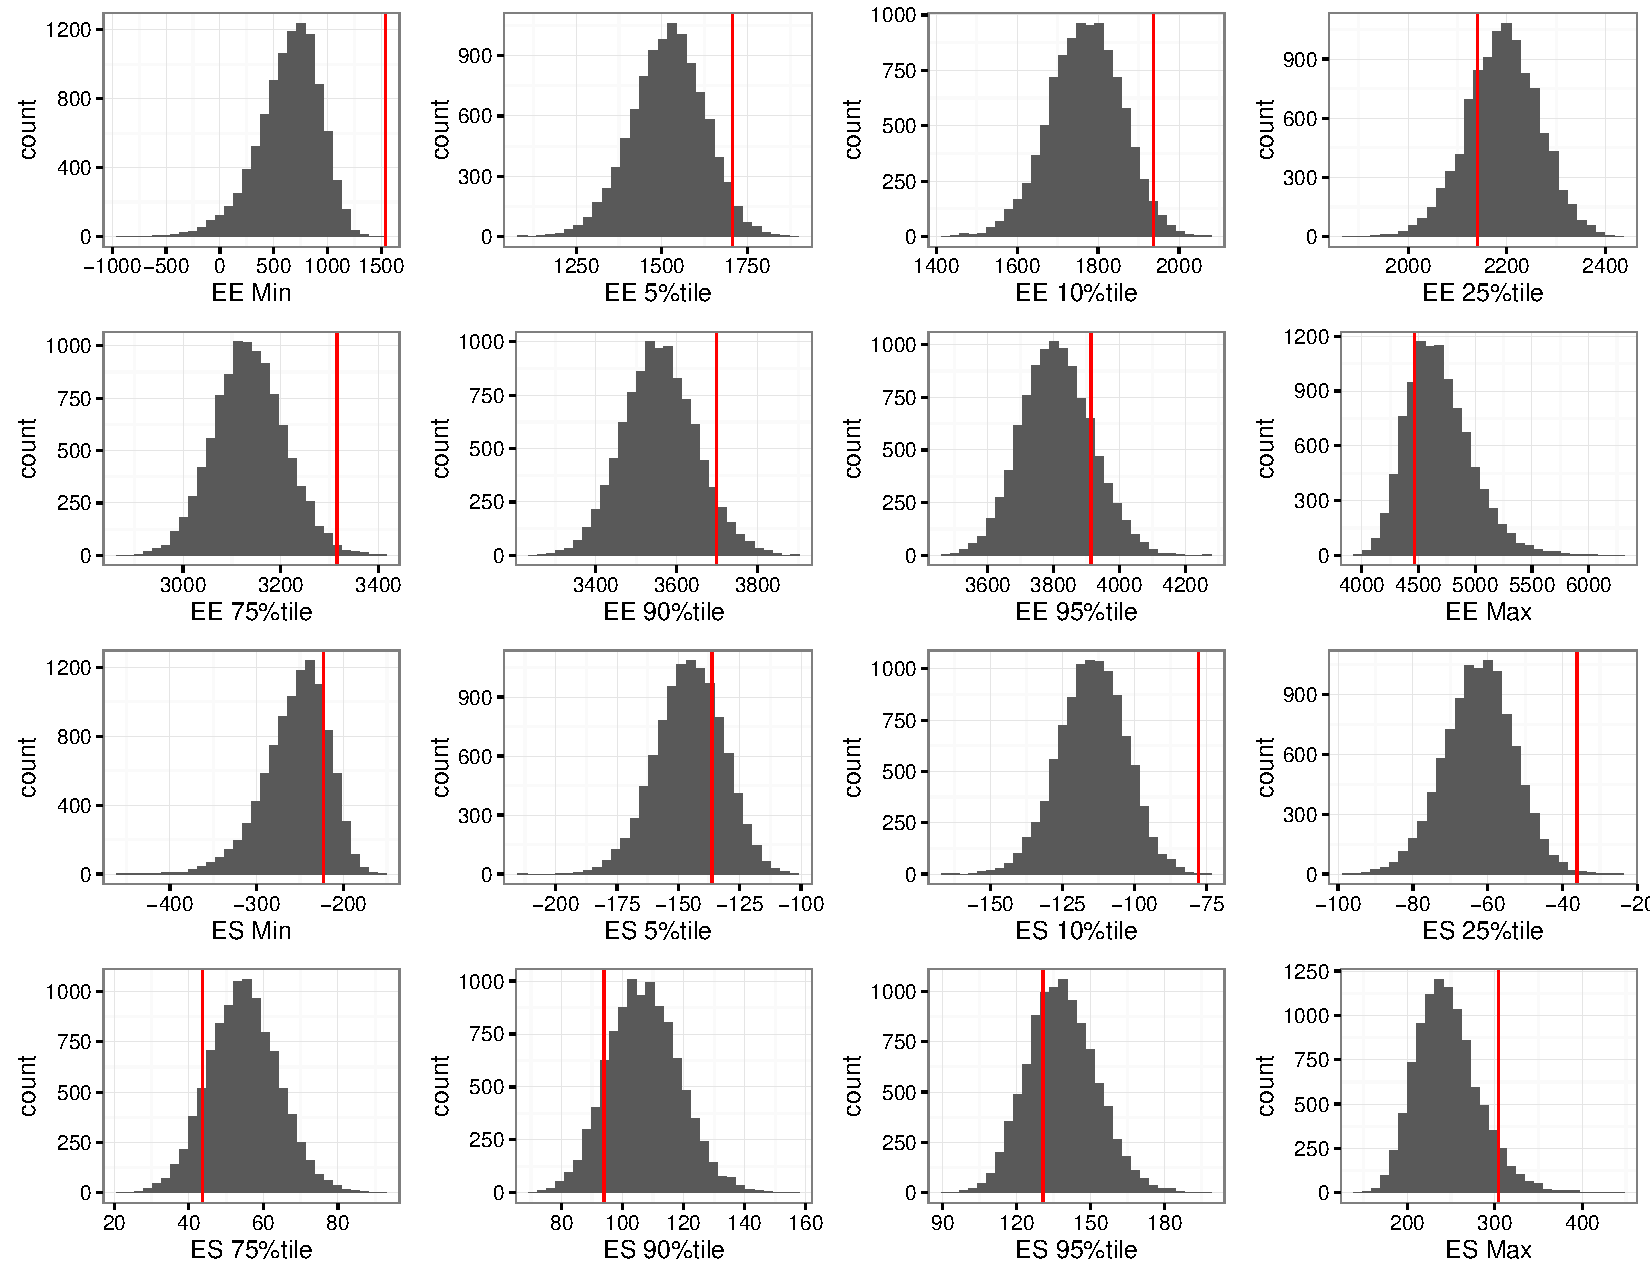
\includegraphics[width=17cm,height=15cm]{manual_figure/wpxdiagbvnb.pdf}
 %  \caption{Posterior Predictive Discrepancy Measures For $X^{EE}$ and $X^{\Delta ES}$ for Model BVN with Bimodal Normal Errors}
 %  \label{wpxdiagbvnb}
 %  \end{figure}
 % %post pred check for W
 %  \begin{figure}
 %  \centering
 %  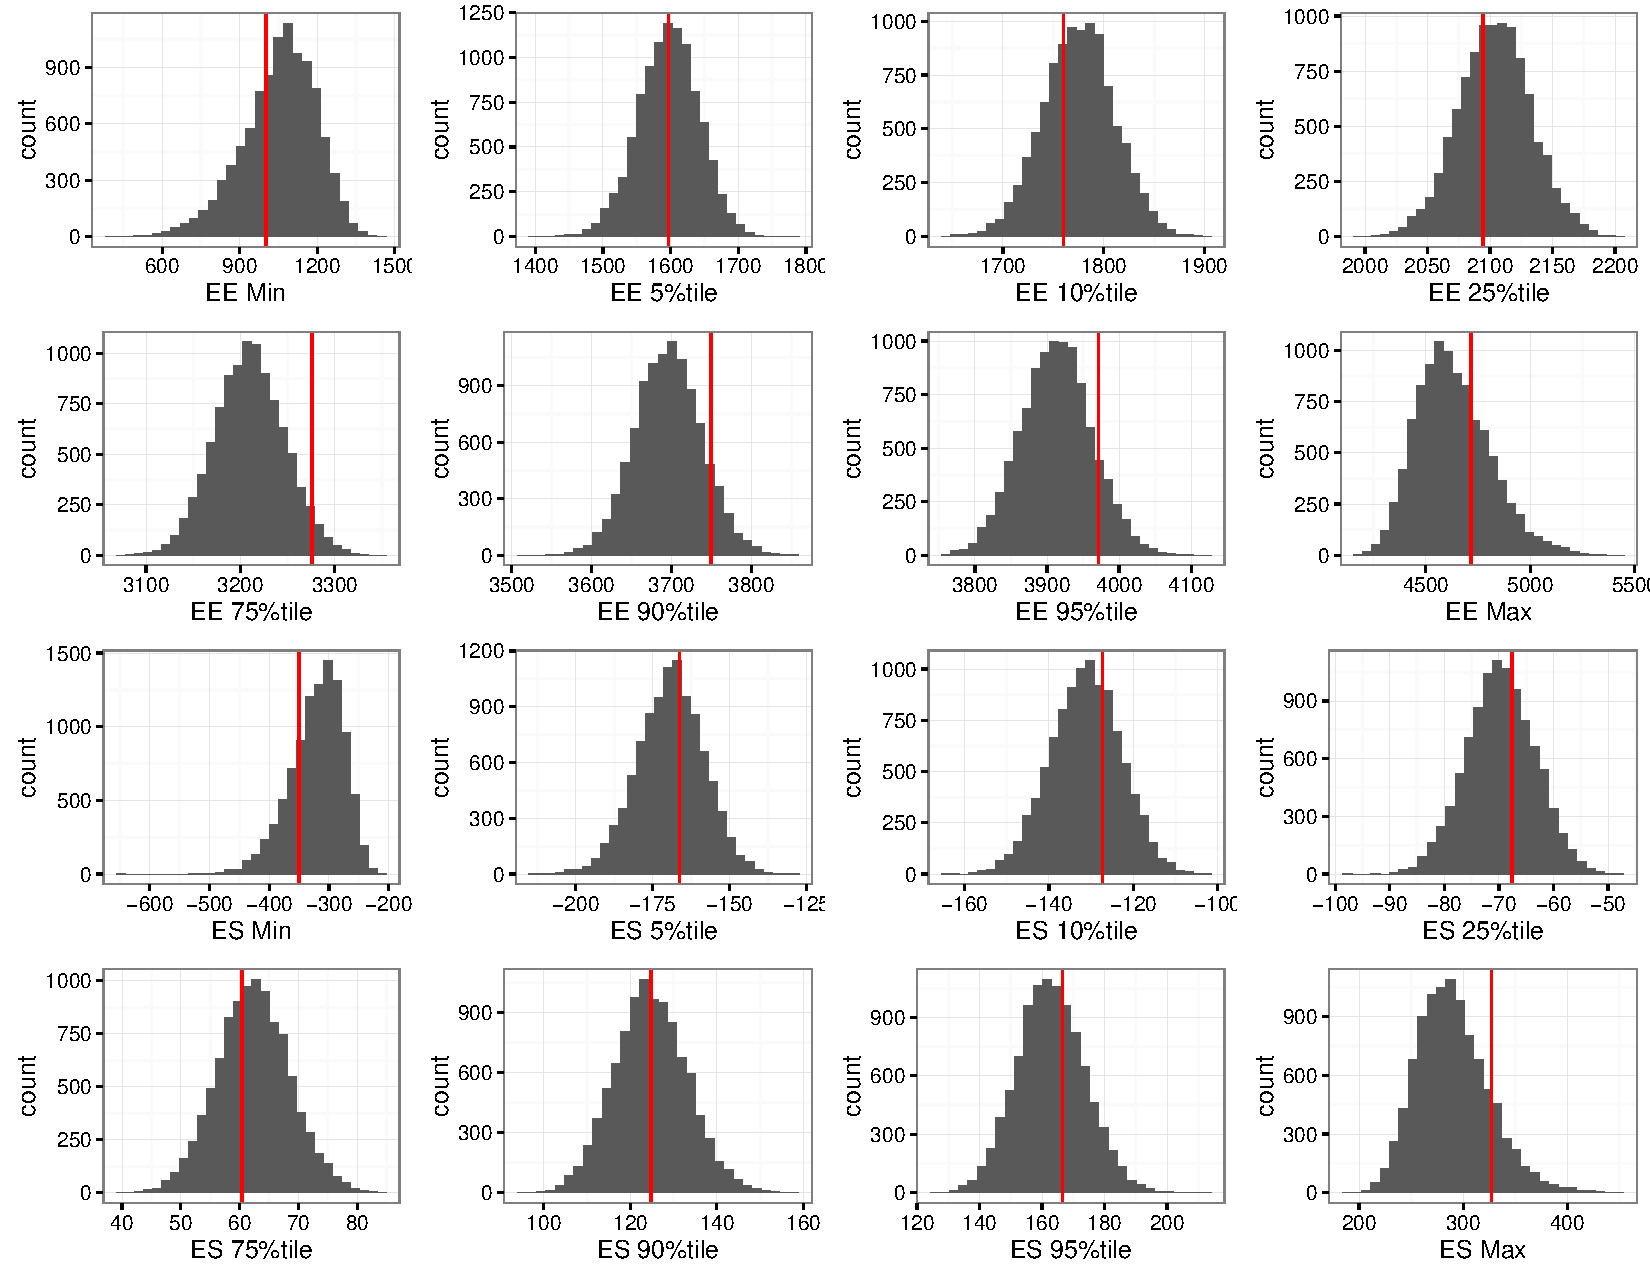
\includegraphics[width=17cm,height=15cm]{manual_figure/wpwdiagbvnb.pdf}
 %  \caption{Posterior Predictive Discrepancy Measures For $W^{EE}$ and $W^{\Delta ES}$ for Model BVN with Bimodal Normal Errors}
 %  \label{wpwdiagbvnb}
 %  \end{figure}
 % %post pred check for Y
 %  \begin{figure}
 %  \centering
 %  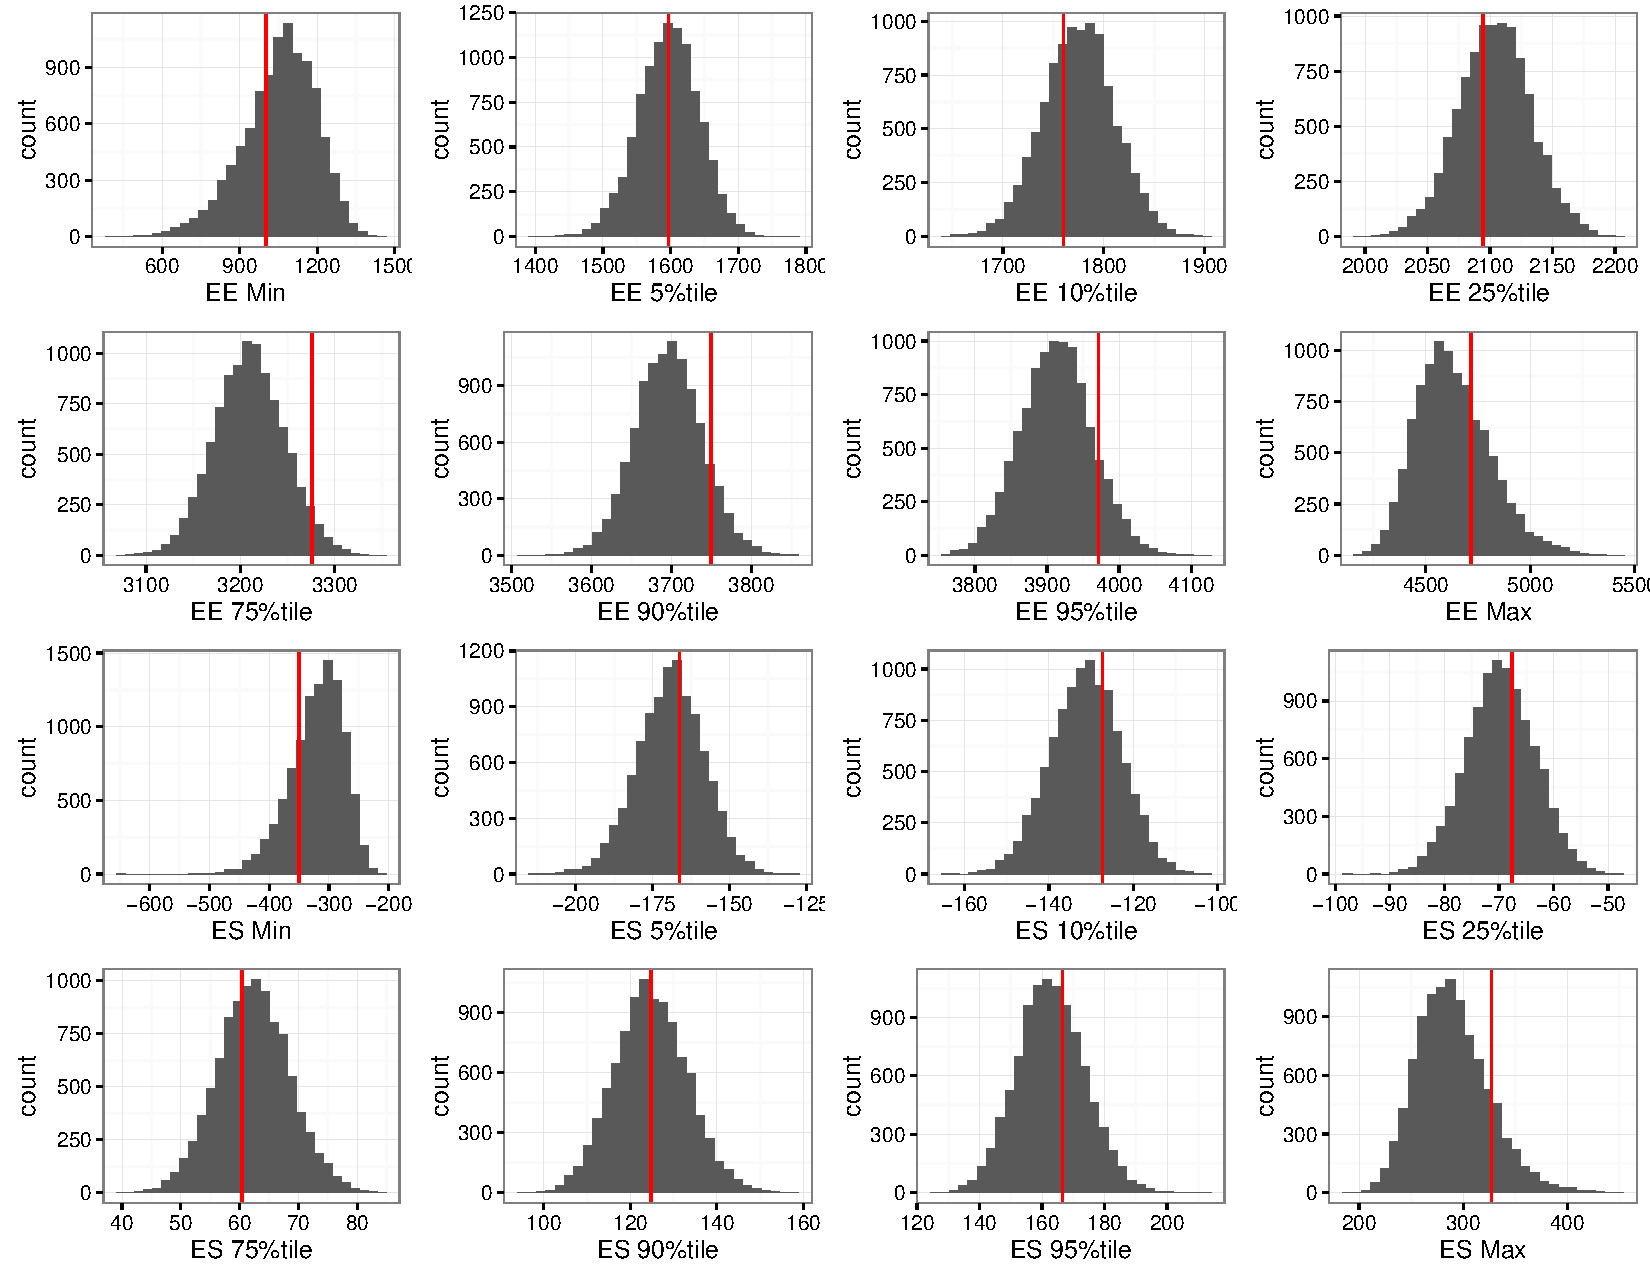
\includegraphics[width=17cm,height=15cm]{manual_figure/wpydiagbvnb.pdf}
 %  \caption{Posterior Predictive Discrepancy Measures For $Y^{EE}$ and $Y^{\Delta ES}$ for Model BVN with Bimodal Normal Errors}
 %  \label{wpydiagbvnb}
 %  \end{figure}



  % \begin{figure}
  % \centering
  % 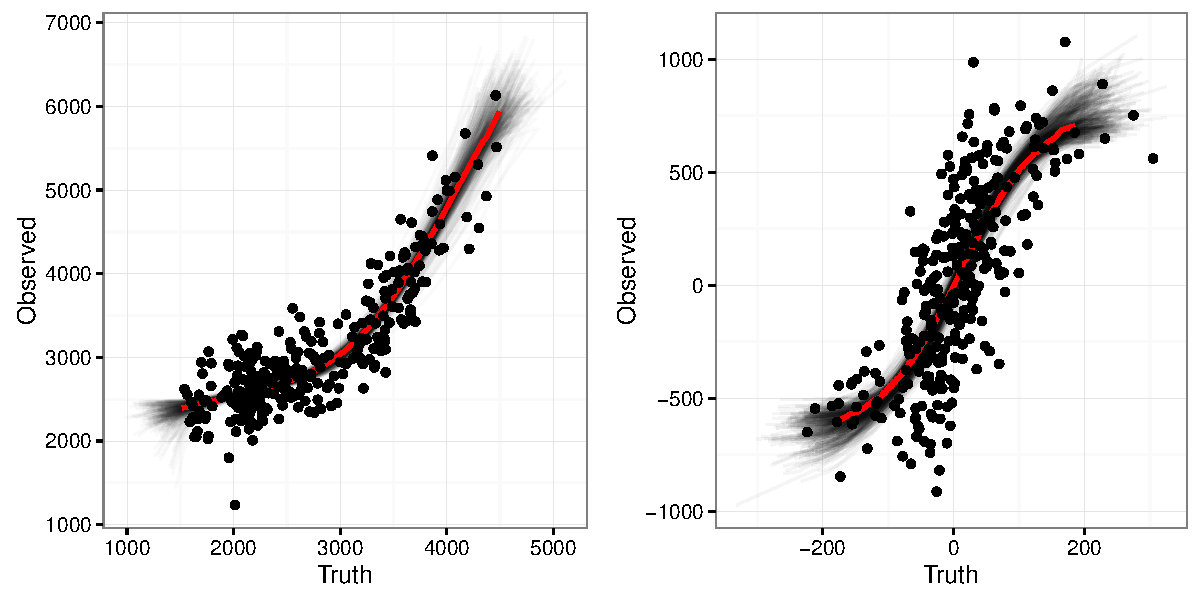
\includegraphics[width=17cm,height=8cm]{manual_figure/predbvnx.pdf}
  % \caption{Spline function for Model BVN with Normal Errors}
  % \label{predbvnx}
  % \end{figure}

  \begin{figure}
  \centering
  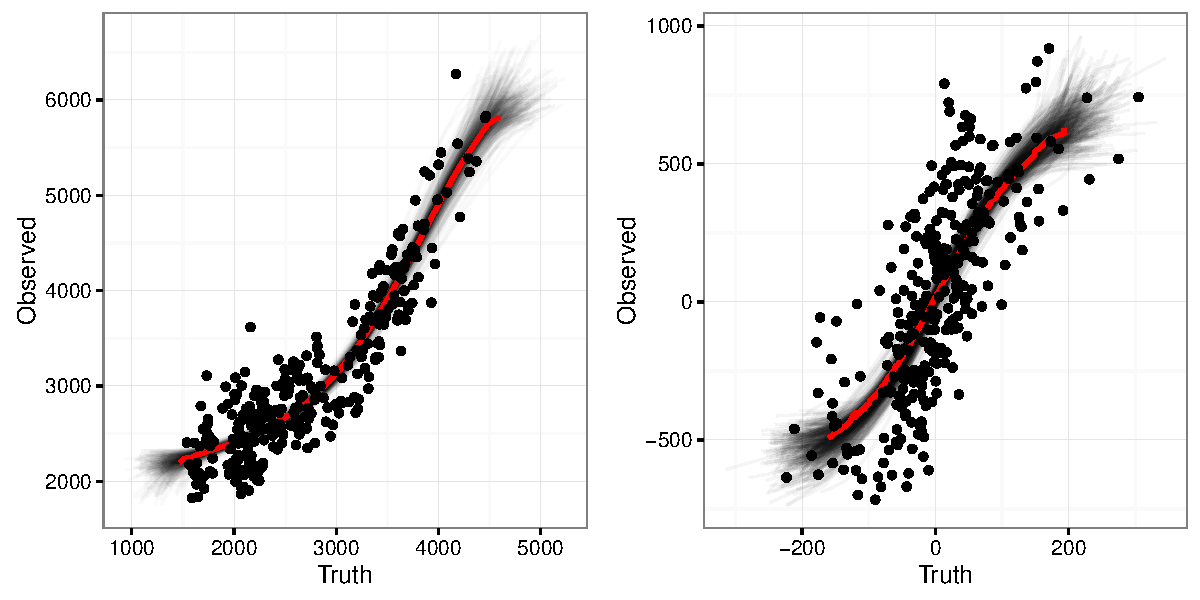
\includegraphics[width=17cm,height=8cm]{manual_figure/predbvnsx.pdf}
  \caption{Spline function for Model BVNS with Skewed Errors}
  \label{predbvnsx}
  \end{figure}

  % \begin{figure}
  % \centering
  % 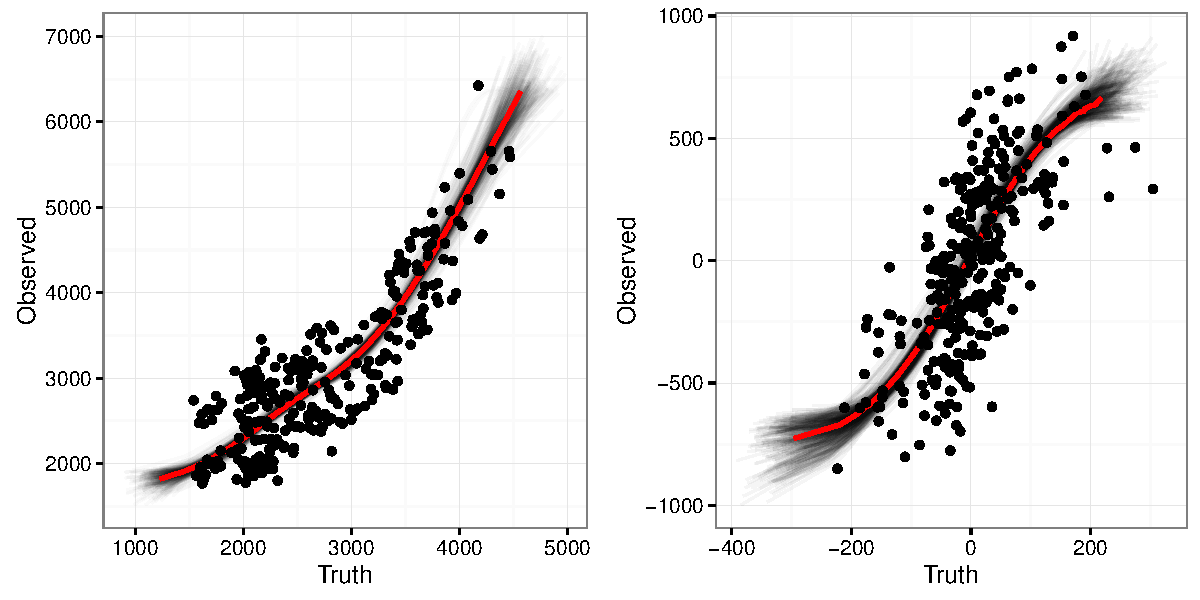
\includegraphics[width=17cm,height=8cm]{manual_figure/predbvnbx.pdf}
  % \caption{Spline function for Model BVN with Bimodal Errors}
  % \label{predbvnbx}
  % \end{figure}



% \subsection{N{\"a}ive Model}
% %In this section we present results for when the within person variability error term is placed within the function $m_{\cdot}(\cdot)$, which is the correct specification. 
% 
% For the three of the simulated data sets, we ran 3 chains of 10,000 iterations each with 2000 burn in. JAGS automatically selects dispersed starting values. The chains for both of the models had Gelman-Rubin diagnostics of one's for all parameters and the trace plots have good mixing with little autocorrelation. 
% 
% Tables \ref{m0wpestimates},\ref{m0swpestimates},\ref{m0bwpestimates} give posterior summaries for parameters for the n{\"a}ive model with normal, skewed and bimodal errors, respectively. Overall, results look similar. Under all 3 data sets, the n{\"a}ive model is able to estimate the linear, error free coefficients. Slopes for $X^{EE}$ and $X^{\Delta ES}$ were different for each data set with the bimodal errors have the largest values. The bimodal errors also had lower values for the regression error variances.
% 
% 
% Figures \ref{ydiag0wp},\ref{ydiag0swp},\ref{ydiag0bwp} gives quantiles from the posterior predictive distribution for $Y$ for EE and $\Delta$ES for simulated data with normal, skewed, and bimodal errors respectively. We computed the posterior predictive distributions using the equation below. The vertical line in each plot indicates the truth in the simulated data. If the plotted distribution covers this truth it indicates the model captures that quantity of interest. If not, it indicates a shortcoming of the model as there is a discrepany between the truth and the model. Figure \ref{ydiag0wp} shows that all values of EE are being underestimated and not capturing the truth at all for the most part. Values for $\Delta$ES actually look okay, but for both EE and $\Delta$ES these distributions have very high variance. These issues could be coming from a variety of places in the model including the mean functions for $Y$ and the distributional assumptions. Since we are in a measurement error situation, we know that using the observed $W$ as the truth is not a good idea, and we should implement a measurement error model. Figures \ref{ydiag0swp},\ref{ydiag0bwp} shows similar results. 
% 
% The goal here was to show that assuming values are measured with no error when error is in fact present, can cause serious problems, in addition to poor performance in terms of predicted mean squared error (PMSE). We realize the issue of not having an acceptable mean structure could confound this conclusion, which is why we present a ME model with the same mean structure as this model next.
% 
%  \begin{align}
%    \label{ypostpred0}
%    p(Y^*|Y,W) &= \int p(Y^*|W,\theta) p(\theta|W,Y) d\theta
%  \end{align}
% 
% \begin{table}[ht]
% \centering
% \begin{tabular}{rrrrrr|r}
%   \hline
%  & 2.5\% & 25\% & 50\% & 75\% & 97.5\% & Truth\\ 
%   \hline
% $\beta_{0,ee}$ & 277.71 & 462.09 & 555.58 & 650.60 & 830.17 \\ 
%   $\beta_{1,ee}$ & 0.74 & 0.78 & 0.79 & 0.81 & 0.85 \\ 
%   $\beta_{0,es}$ & -307.64 & -160.92 & -90.00 & -20.16 & 117.63 \\ 
%   $\beta_{1,es}$ & 3.38 & 3.60 & 3.71 & 3.82 & 4.03 \\ 
%   $\sigma_{yee}$ & 466.10 & 483.20 & 492.71 & 502.63 & 522.21 \\ 
%   $\sigma_{yes}$ & 327.54 & 339.66 & 346.24 & 353.04 & 366.78 \\ 
%   $\gamma_{1,ee}$ & 240.54 & 294.45 & 322.45 & 350.14 & 403.34 & 300\\ 
%   $\gamma_{2,ee}$ & 7.64 & 12.75 & 15.47 & 18.27 & 23.78 & 14 \\ 
%   $\gamma_{3,ee}$ & -14.23 & -10.11 & -7.86 & -5.64 & -1.51 & -7 \\ 
%   $\gamma_{1,es}$ & -277.99 & -241.98 & -222.91 & -204.06 & -167.10 & -200 \\ 
%   $\gamma_{2,es}$ & 5.37 & 9.17 & 11.18 & 13.17 & 17.39 & 8 \\ 
%   $\gamma_{3,es}$ & -8.14 & -4.99 & -3.33 & -1.76 & 1.23 & -5\\ 
%    \hline
% \end{tabular}
% \caption{Parameter estimates for Model 0 for normal errors with correct specification of within person errors}
% \label{m0wpestimates}
% \end{table}
% 
% 
% \begin{table}[ht]
% \centering
% \begin{tabular}{rrrrrr|r}
%   \hline
%  & 2.5\% & 25\% & 50\% & 75\% & 97.5\% & Truth\\ 
%   \hline
% $\beta_{0,ee}$ & 39.20 & 228.72 & 329.47 & 429.62 & 622.31 \\ 
%   $\beta_{1,ee}$ & 0.91 & 0.94 & 0.96 & 0.98 & 1.02 \\ 
%   $\beta_{0,es}$ & -182.65 & -46.24 & 20.78 & 85.59 & 210.74 \\ 
%   $\beta_{1,es}$ & 2.66 & 2.86 & 2.97 & 3.07 & 3.27 \\ 
%   $\sigma_{yee}$ & 455.71 & 472.67 & 481.86 & 491.63 & 511.03 \\ 
%   $\sigma_{yes}$ & 312.59 & 324.02 & 330.35 & 336.95 & 350.18 \\ 
%   $\gamma_{1,ee}$ & 188.54 & 241.12 & 268.70 & 296.06 & 349.57 & 300\\ 
%   $\gamma_{2,ee}$ & 2.31 & 7.72 & 10.40 & 13.25 & 18.55 & 14\\ 
%   $\gamma_{3,ee}$ & -16.59 & -12.25 & -10.05 & -7.91 & -3.56 & -7\\ 
%   $\gamma_{1,es}$ & -286.35 & -251.71 & -233.56 & -215.41 & -180.68 & -200\\ 
%   $\gamma_{2,es}$ & 1.96 & 5.69 & 7.53 & 9.32 & 13.10 & 8\\ 
%   $\gamma_{3,es}$ & -7.56 & -4.67 & -3.17 & -1.67 & 1.27 & -5\\ 
%    \hline
%    \end{tabular}
% \caption{Parameter estimates for Model 0 for skewed errors with correct specification of within person errors}
% \label{m0swpestimates}
% \end{table}
% 
% 
% \begin{table}[ht]
% \centering
% \begin{tabular}{rrrrrr|r}
%   \hline
%  & 2.5\% & 25\% & 50\% & 75\% & 97.5\% & Truth\\
%   \hline
% $\beta_{0,ee}$ & -214.68 & -60.93 & 15.11 & 93.78 & 236.57 \\ 
%   $\beta_{1,ee}$ & 0.99 & 1.02 & 1.03 & 1.05 & 1.07 \\ 
%   $\beta_{0,es}$ & -57.37 & 31.59 & 81.77 & 131.86 & 232.59 \\ 
%   $\beta_{1,es}$ & 3.22 & 3.36 & 3.44 & 3.51 & 3.65 \\ 
%   $\sigma_{yee}$ & 339.11 & 351.89 & 358.93 & 366.09 & 380.58 \\ 
%   $\sigma_{yes}$ & 231.48 & 239.98 & 244.66 & 249.57 & 259.42 \\ 
%   $\gamma_{1,ee}$ & 205.14 & 244.14 & 264.19 & 284.56 & 323.20 & 300\\ 
%   $\gamma_{2,ee}$ & 9.12 & 13.16 & 15.22 & 17.28 & 21.15 & 14\\ 
%   $\gamma_{3,ee}$ & -14.28 & -11.31 & -9.66 & -8.08 & -5.03 & -7\\ 
%   $\gamma_{1,es}$ & -226.15 & -200.38 & -186.83 & -173.27 & -147.33 &-200 \\ 
%   $\gamma_{2,es}$ & 0.78 & 3.58 & 5.02 & 6.38 & 8.94 & 8\\ 
%   $\gamma_{3,es}$ & -7.18 & -5.05 & -3.97 & -2.86 & -0.66 & -5\\ 
%    \hline
% \end{tabular}
% \caption{Parameter estimates for Model 0 for bimodal errors with correct specification of within person errors}
% \label{m0bwpestimates}
% \end{table}
% 
% 
% 
% 
% \begin{figure}
%  \centering
%  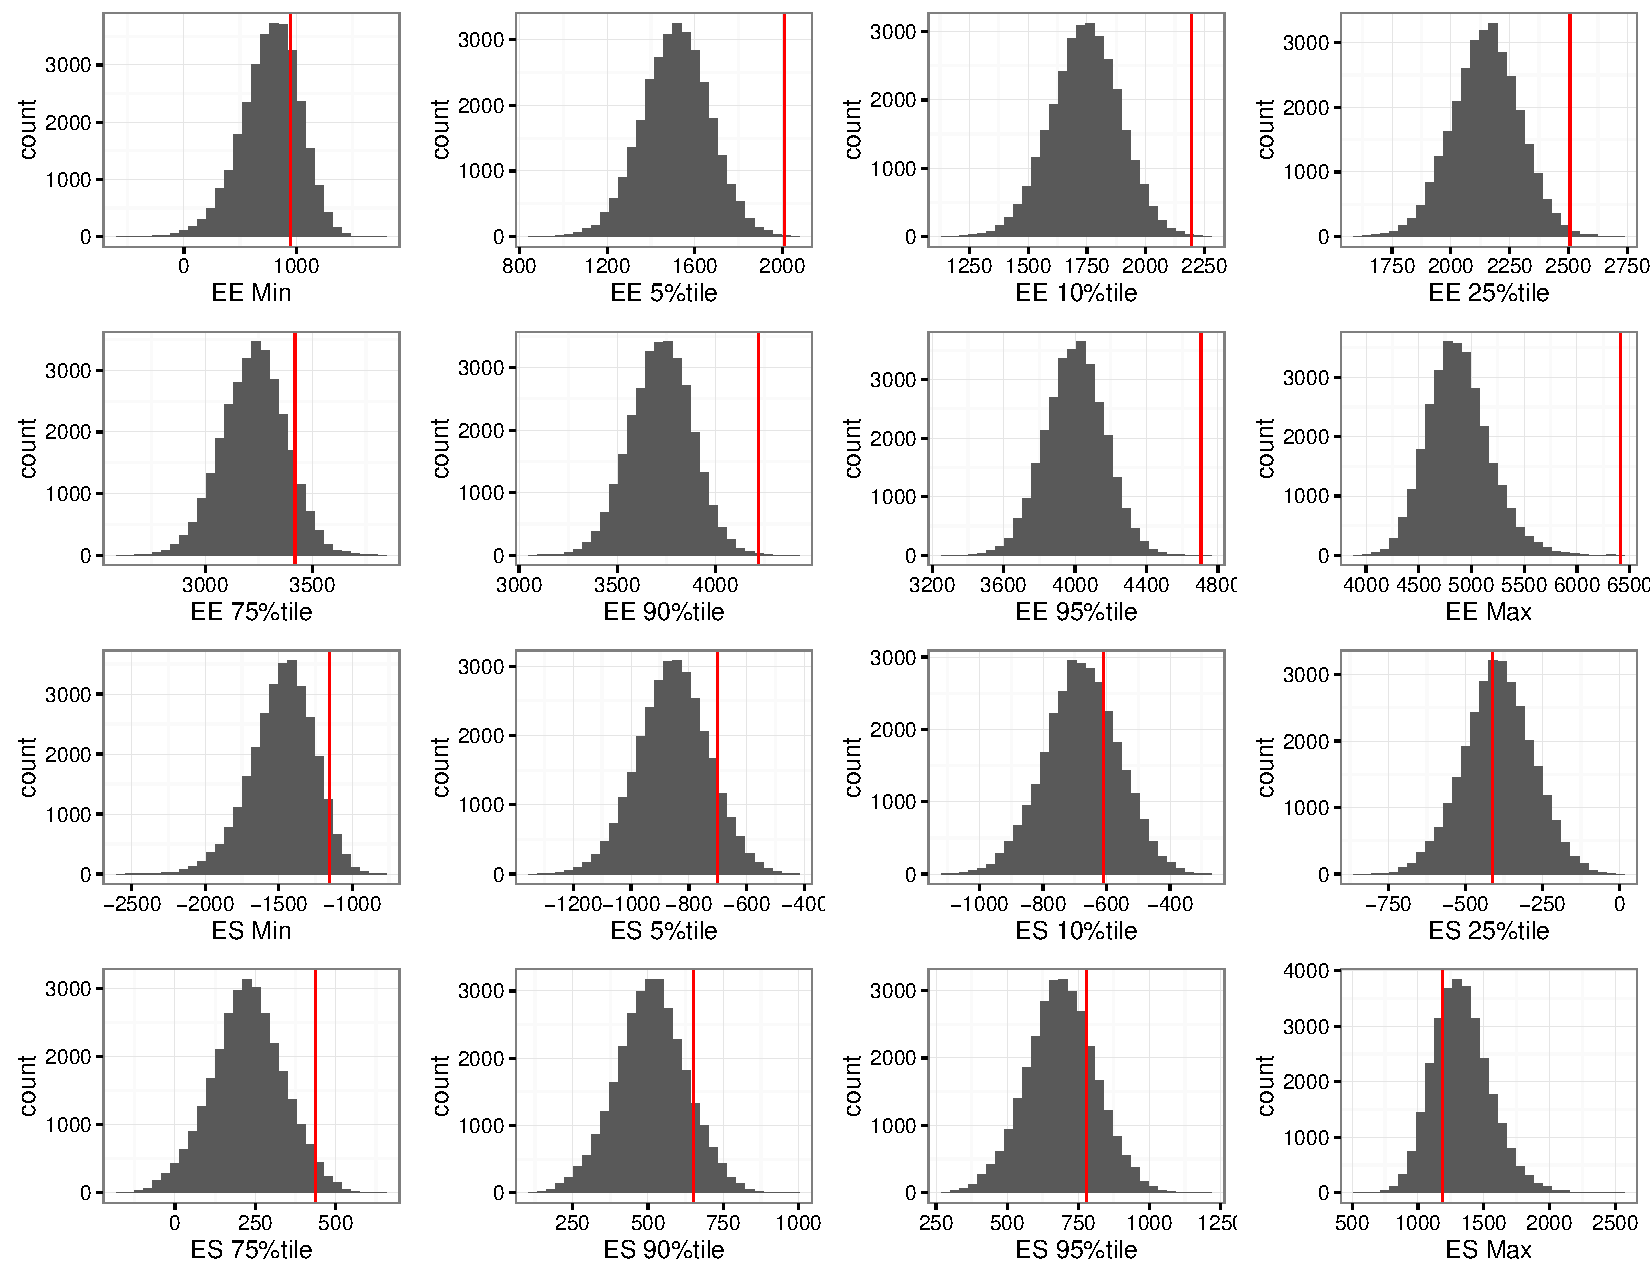
\includegraphics[width=17cm,height=15cm]{manual_figure/wpydiag0.pdf}
%  \caption{Posterior Predictive Discrepancy Measures For $Y^{EE}$ and $Y^{\Delta ES}$ for Model 0 with Normal Errors with correct specification of within person errors}
%  \label{ydiag0wp}
%  \end{figure}
% 
% \begin{figure}
%  \centering
%  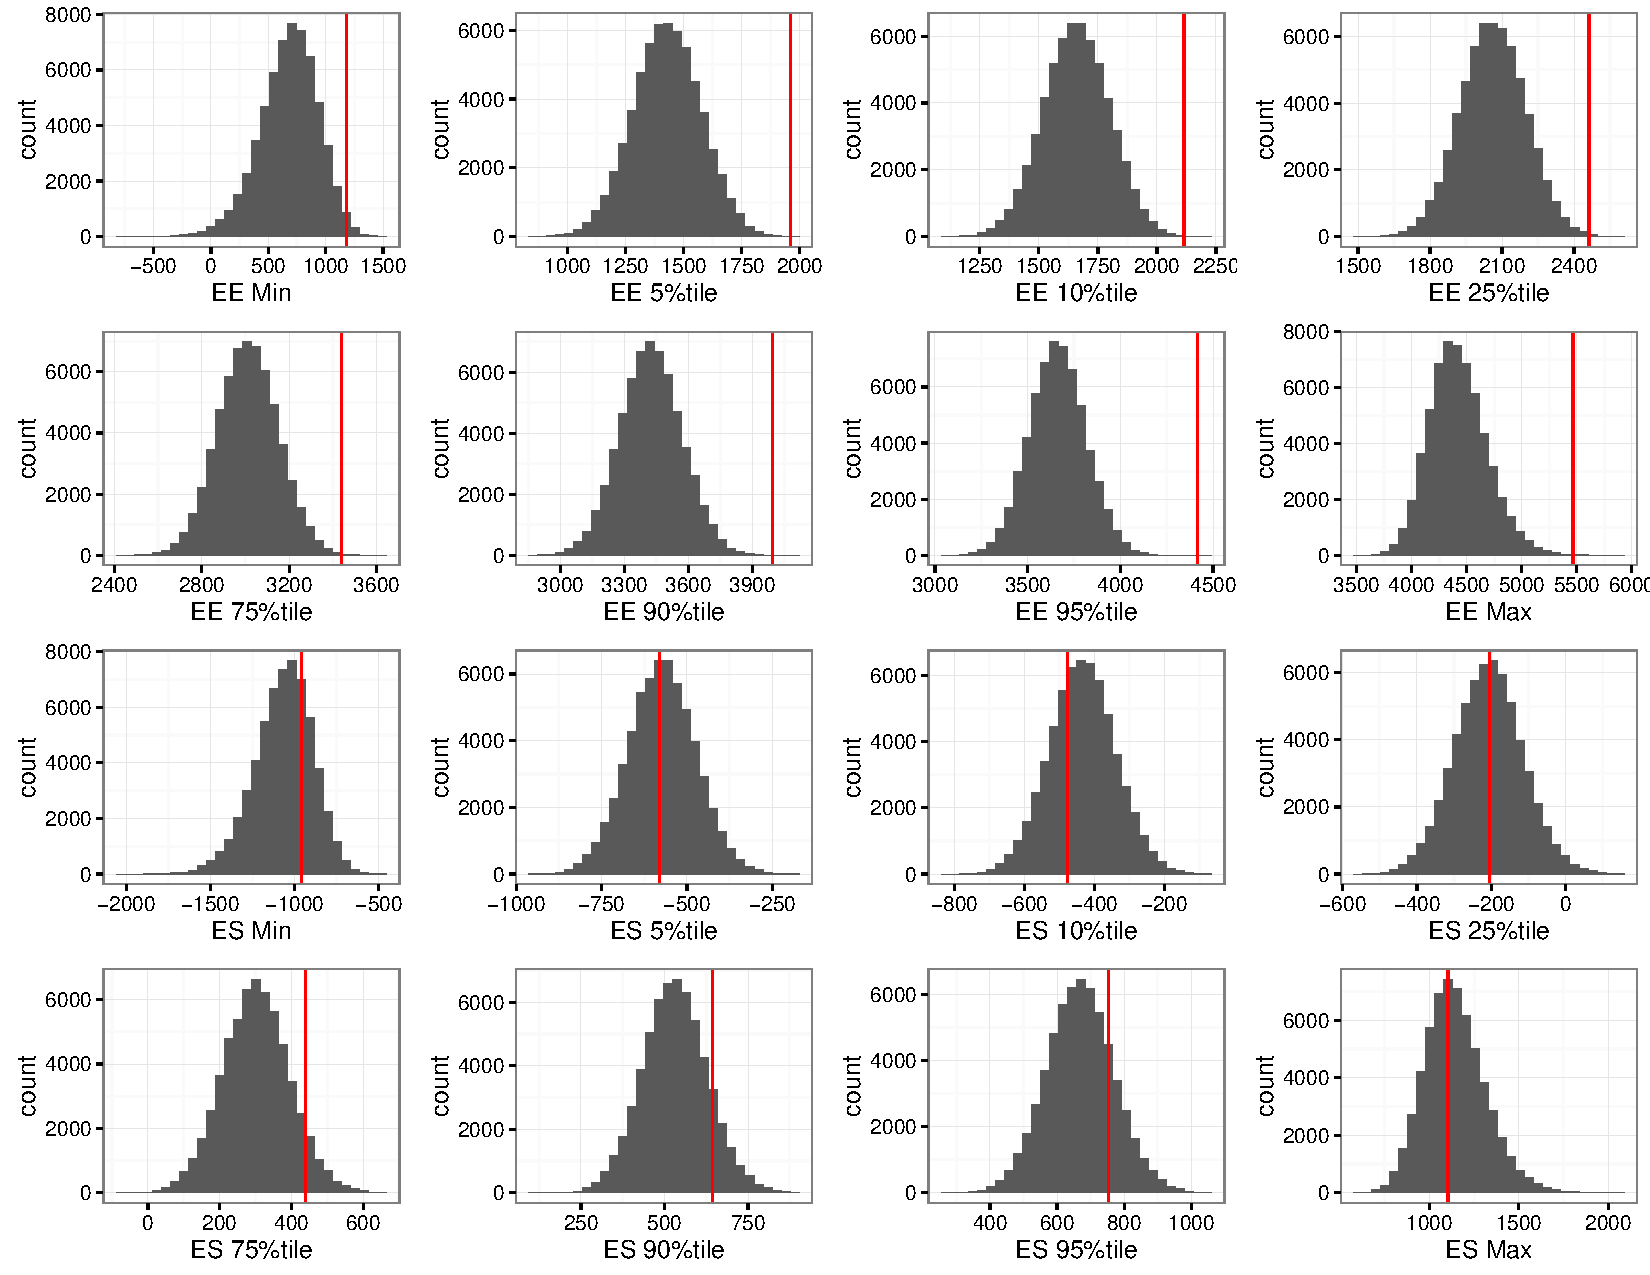
\includegraphics[width=17cm,height=15cm]{manual_figure/wpydiag0s.pdf}
%  \caption{Posterior Predictive Discrepancy Measures For $Y^{EE}$ and $Y^{\Delta ES}$ for Model 0 with Skewed Normal Errors with correct specification of within person errors}
%  \label{ydiag0swp}
%  \end{figure}
% 
%  \begin{figure}
%  \centering
%  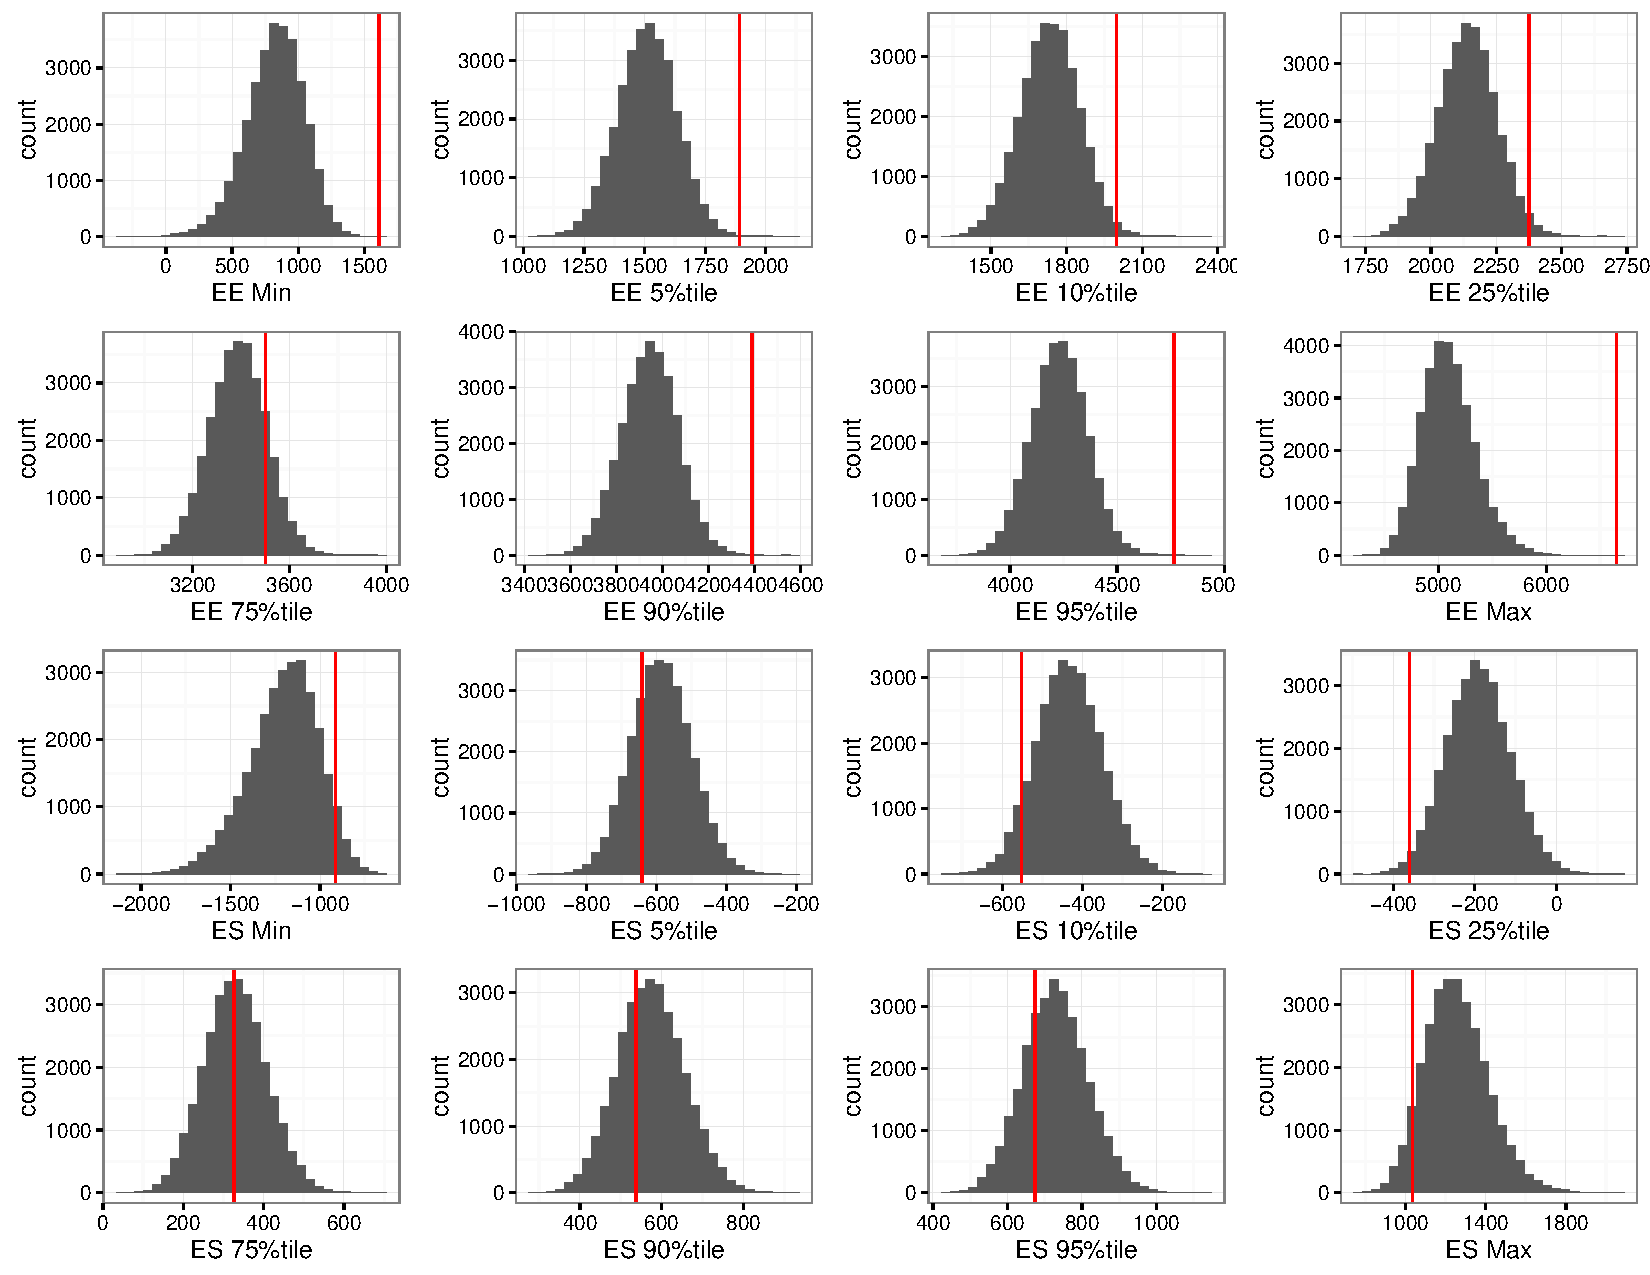
\includegraphics[width=17cm,height=15cm]{manual_figure/wpydiag0b.pdf}
%  \caption{Posterior Predictive Discrepancy Measures For $Y^{EE}$ and $Y^{\Delta ES}$ for Model 0 with Bimodal Errors with correct specification of within person errors}
%  \label{ydiag0bwp}
%  \end{figure}
% 
% 
% %-------------------------------------------------------
% %-------------------------------------------------------
% %-------------------Model 1-----------------------------
% %-------------------------------------------------------
% %-------------------------------------------------------
% 
% 
% 
% \subsection{Model 1}
% 
% Like in Model 0, we ran 3 chains of 10,000 iterations each with 2000 burn in and all parameters had Gelman-Rubin diagnostics of less than 1.02 and trace plots indicated good mixing.
% 
% Tables \ref{m1wpestimates},\ref{m1swpestimates},\ref{m1bwpestimates} give posterior summaries for parameters for the simple model under normal, skewed, and bimodal errors respectively. Regression coefficients look similar based on both types of errors. The only time the truth isn't covered by the 95\% credible interval is for gender in $\Delta$ES under the skewed errors. 
% 
% 
% Figures \ref{wpxdiag1} and \ref{wpxdiag1s} give posterior predictive checks for the latent variables $X^{EE}$ and $X^{\Delta ES}$.  Both sets of plots look okay except for the minimum and maximum values. This is somewhat surprising considering this model uses only a single bivariate normal distribution to model the latent variables. One issue, however, is the amount of variance in these plots. For a given percentile the posterior predictive distribution gives a wide range of values and for the minimum values of EI and EE, it gives values close to -1000, which makes no sense in the context of our problem.
% 
% Figures \ref{wpwdiag1} and \ref{wpwdiag1s} give posterior predictive checks for the gold standard measurements $W$ for normal and skewed errors respectively. Figure \ref{wpwdiag1} shows no signs of issues which is not surprising since this model assumes normal measurement errors. Figure \ref{wpwdiag1s} also looks good except there are some extreme outliers in $\Delta$ES measures.
% 
% Figures \ref{wpydiag1} and \ref{wpydiag1s} give posterior predictive checks for the gold standard measurements $W$ for normal and skewed errors respectively. Figure \ref{wpydiag1} shows no major signs of problems, which like before, is expected because the truth is normal errors. The variance for the percentiles is still large though. Figure \ref{wpydiag1s} shows in the small percentiles of EE as well as the 75th and maximum. For $\Delta$ES, only the 5th  and 90th percentiles look okay. One culprit for this is misspecification of the measurement errors, but this could be compounded by assuming a linear structure and/or the normality assumption on the latent variables.
% 
% 
% 
% PMSE for this simulated data and these fitted models is given in Table \ref{pmse2}.
% 
% 
% 
% \begin{table}[ht]
% \centering
% \begin{tabular}{rrrrrr|r}
%   \hline
%  & 2.5\% & 25\% & 50\% & 75\% & 97.5\% & Truth\\ 
%   \hline
% $\beta_{0,ee}$ & 83.43 & 286.31 & 392.49 & 497.99 & 719.08 \\ 
%   $\beta_{1,ee}$ & 0.80 & 0.84 & 0.86 & 0.88 & 0.92 \\ 
%   $\beta_{0,es}$ & -320.83 & -158.99 & -78.38 & 5.59 & 178.58 \\ 
%   $\beta_{1,es}$ & 4.14 & 4.47 & 4.66 & 4.85 & 5.23 \\ 
%   $\mu_x^{EE}$ & 2617.25 & 2670.55 & 2698.99 & 2727.88 & 2781.14 \\ 
%   $\mu_x^{\Delta ES}$ & -7.77 & -1.29 & 2.16 & 5.63 & 12.07 \\ 
%   $\sigma_{yee}$ & 431.23 & 449.77 & 459.89 & 469.98 & 490.46 \\ 
%   $\sigma_{yes}$ & 303.30 & 316.12 & 323.31 & 330.85 & 345.57 \\ 
%   $\sigma_{wee}$ & 239.31 & 252.22 & 259.48 & 267.14 & 282.67 & 250\\ 
%   $\sigma_{wes}$ & 65.14 & 68.04 & 69.60 & 71.22 & 74.43 & 72.862 \\ 
%   $\sigma_{xee}$ & 652.14 & 689.61 & 710.28 & 731.30 & 775.42 \\ 
%   $\sigma_{xes}$ & 65.97 & 71.11 & 73.95 & 76.92 & 82.93 \\ 
%   $\rho$ & -0.24 & -0.15 & -0.11 & -0.06 & 0.02 \\ 
%   $\gamma_{1,ee}$ & 231.70 & 288.52 & 317.27 & 345.91 & 401.34 & 300\\ 
%   $\gamma_{2,ee}$ & 5.89 & 11.80 & 14.86 & 17.65 & 22.50 & 14\\ 
%   $\gamma_{3,ee}$ & -14.59 & -9.96 & -7.65 & -5.30 & -1.35 & -7\\ 
%   $\gamma_{1,es}$ & -289.47 & -245.90 & -222.68 & -199.28 & -153.92 &-200 \\ 
%   $\gamma_{2,es}$ & 3.59 & 8.33 & 10.79 & 13.19 & 17.77 & 8\\ 
%   $\gamma_{3,es}$ & -9.11 & -5.50 & -3.49 & -1.61 & 2.09 & -5\\ 
%    \hline
% \end{tabular}
% \caption{Parameter estimates for Model 1 for normal errors with correct specification of within person errors}
% \label{m1wpestimates}
% \end{table}
% 
% 
% 
% \begin{table}[ht]
% \centering
% \begin{tabular}{rrrrrr|r}
%   \hline
%  & 2.5\% & 25\% & 50\% & 75\% & 97.5\% & Truth\\ 
%   \hline
% $\beta_{0,ee}$ & -136.25 & 64.01 & 164.19 & 272.76 & 478.66 \\ 
%   $\beta_{1,ee}$ & 0.98 & 1.02 & 1.04 & 1.06 & 1.10 \\ 
%   $\beta_{0,es}$ & -223.94 & -63.11 & 9.64 & 87.16 & 227.35 \\ 
%   $\beta_{1,es}$ & 3.32 & 3.62 & 3.79 & 3.97 & 4.33 \\ 
%   $\mu_x^{EE}$ & 2626.86 & 2680.08 & 2708.93 & 2737.61 & 2792.61 \\ 
%   $\mu_x^{\Delta ES}$ & -7.53 & -0.91 & 2.51 & 5.97 & 12.54 \\ 
%   $\sigma_{yee}$ & 404.01 & 422.30 & 432.51 & 442.74 & 463.17 \\ 
%   $\sigma_{yes}$ & 294.31 & 306.63 & 313.48 & 320.62 & 334.84 \\ 
%   $\sigma_{wee}$ & 247.61 & 260.74 & 268.09 & 275.86 & 291.15 & 250\\ 
%   $\sigma_{wes}$ & 65.28 & 68.23 & 69.86 & 71.55 & 74.98 & 72.862\\ 
%   $\sigma_{xee}$ & 653.95 & 690.93 & 711.49 & 733.06 & 776.22 \\ 
%   $\sigma_{xes}$ & 65.12 & 70.54 & 73.42 & 76.36 & 82.30 \\ 
%   $\rho$ & -0.28 & -0.20 & -0.15 & -0.11 & -0.02 \\ 
%   $\gamma_{1,ee}$ & 181.87 & 236.10 & 265.11 & 293.78 & 348.64 & 300\\ 
%   $\gamma_{2,ee}$ & 0.52 & 6.32 & 9.30 & 12.20 & 17.84 & 14\\ 
%   $\gamma_{3,ee}$ & -16.95 & -12.98 & -10.62 & -8.17 & -3.49 & -7\\ 
%   $\gamma_{1,es}$ & -290.13 & -249.26 & -228.14 & -206.89 & -165.11 & -200 \\ 
%   $\gamma_{2,es}$ & 1.69 & 5.58 & 7.74 & 9.95 & 13.94 & 8 \\ 
%   $\gamma_{3,es}$ & -8.47 & -5.00 & -3.20 & -1.38 & 1.88 & -5\\ 
%   \hline
%    \end{tabular}
% \caption{Parameter estimates for Model 1 for skewed errors with correct specification of within person errors}
% \label{m1swpestimates}
% \end{table}
% 
% 
% \begin{table}[ht]
% \centering
% \begin{tabular}{rrrrrr|r}
%   \hline
%  & 2.5\% & 25\% & 50\% & 75\% & 97.5\% & Truth\\
%   \hline
% $\beta_{0,ee}$ & -341.79 & -200.87 & -116.19 & -39.05 & 136.63 \\ 
%   $\beta_{1,ee}$ & 1.05 & 1.08 & 1.10 & 1.11 & 1.14 \\ 
%   $\beta_{0,es}$ & -110.42 & 14.56 & 83.97 & 146.56 & 256.27 \\ 
%   $\beta_{1,es}$ & 3.44 & 3.63 & 3.74 & 3.84 & 4.05 \\ 
%   $\mu_x^{EE}$ & 2586.74 & 2641.17 & 2669.76 & 2698.30 & 2753.33 \\ 
%   $\mu_x^{\Delta ES}$ & -14.49 & -7.48 & -3.78 & -0.15 & 6.79 \\ 
%   $\sigma_{yee}$ & 261.87 & 278.59 & 287.30 & 296.20 & 314.10 \\ 
%   $\sigma_{yes}$ & 225.11 & 234.57 & 239.61 & 244.85 & 255.51 \\ 
%   $\sigma_{wee}$ & 184.23 & 196.59 & 203.62 & 210.91 & 225.74 & 250 \\ 
%   $\sigma_{wes}$ & 49.52 & 51.64 & 52.84 & 54.11 & 56.59 & 72.862\\ 
%   $\sigma_{xee}$ & 668.24 & 704.13 & 724.60 & 745.56 & 788.54 \\ 
%   $\sigma_{xes}$ & 78.68 & 83.62 & 86.39 & 89.34 & 95.14 \\ 
%   $\rho$ & -0.06 & 0.02 & 0.06 & 0.11 & 0.18 \\ 
%   $\gamma_{1,ee}$ & 194.85 & 233.93 & 254.71 & 275.39 & 315.39 & 300\\ 
%   $\gamma_{2,ee}$ & 7.67 & 12.10 & 14.25 & 16.33 & 19.90 & 14\\ 
%   $\gamma_{3,ee}$ & -14.85 & -11.73 & -10.11 & -8.38 & -4.85 & -7\\ 
%   $\gamma_{1,es}$ & -236.86 & -205.53 & -188.75 & -171.75 & -139.94 & -200 \\ 
%   $\gamma_{2,es}$ & 0.30 & 3.10 & 4.84 & 6.56 & 10.24 & 8\\ 
%   $\gamma_{3,es}$ & -7.81 & -5.19 & -3.74 & -2.24 & 0.48 & -5\\ 
%   \hline
% \end{tabular}
% \caption{Parameter estimates for Model 1 for bimodal errors with correct specification of within person errors}
% \label{m1bwpestimates}
% \end{table}
% 
% 
%  %post pred check for X
%  \begin{figure}
%   \centering
%   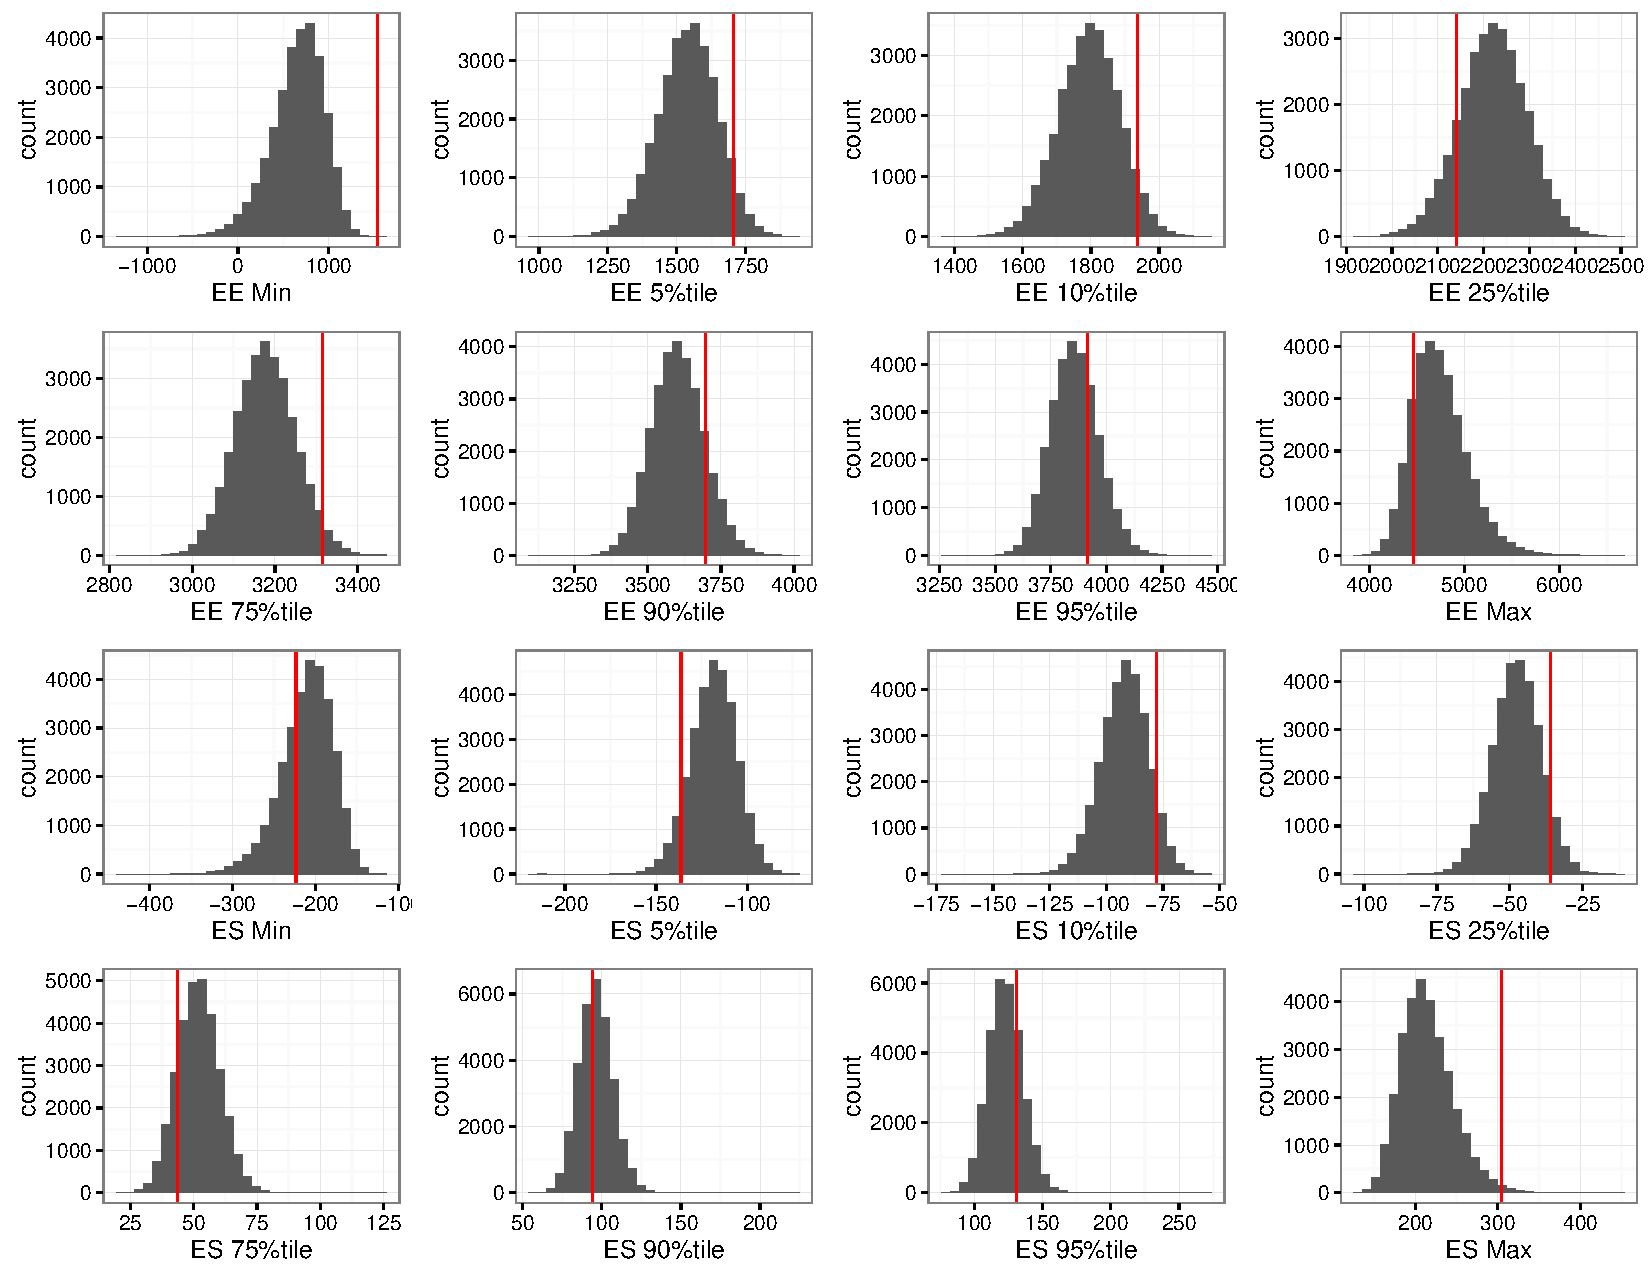
\includegraphics[width=17cm,height=15cm]{manual_figure/wpxdiag1.pdf}
%   \caption{Posterior Predictive Discrepancy Measures For $X^{EE}$ and $X^{\Delta ES}$ for Model 1 with Normal Errors}
%   \label{wpxdiag1}
%   \end{figure}
%  %post pred check for W
%   \begin{figure}
%   \centering
%   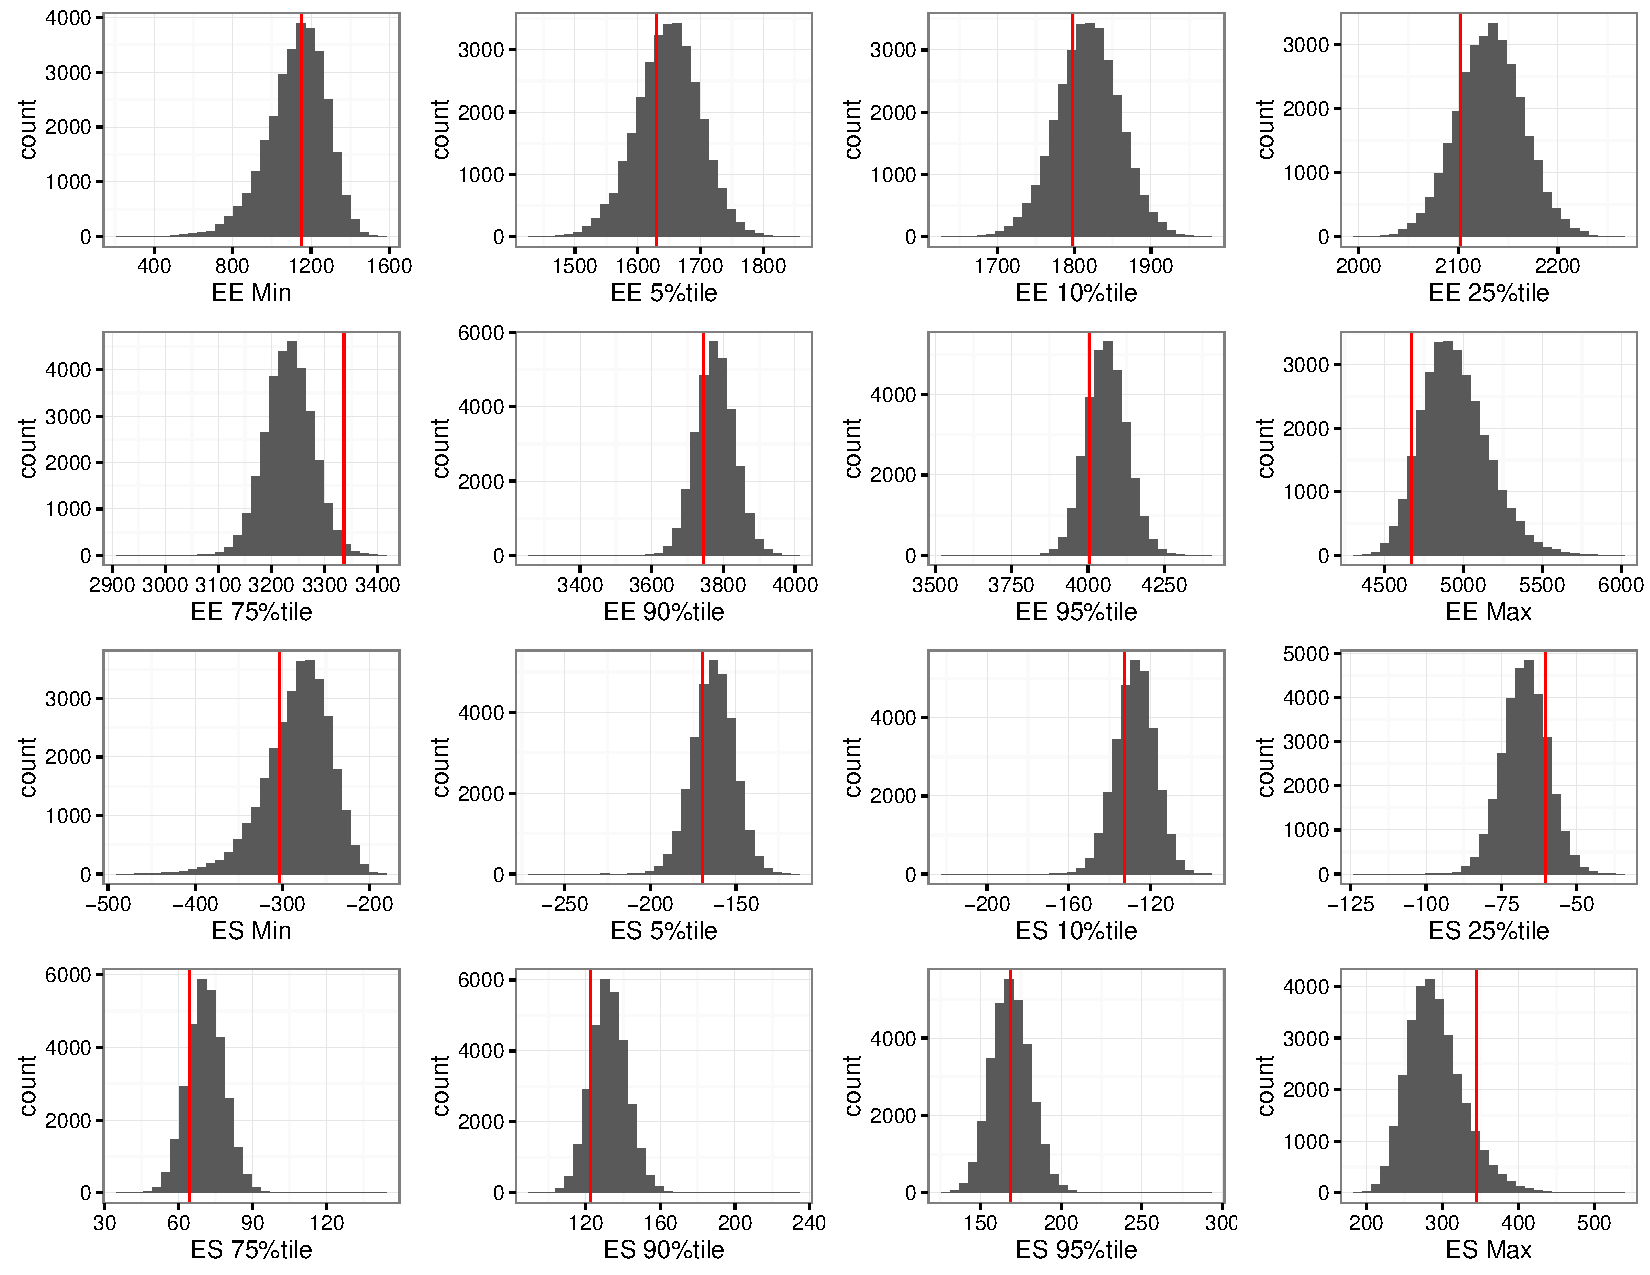
\includegraphics[width=17cm,height=15cm]{manual_figure/wpwdiag1.pdf}
%   \caption{Posterior Predictive Discrepancy Measures For $W^{EE}$ and $W^{\Delta ES}$ for Model 1 with Normal Errors}
%   \label{wpwdiag1}
%   \end{figure}
%  %post pred check for Y
%   \begin{figure}
%   \centering
%   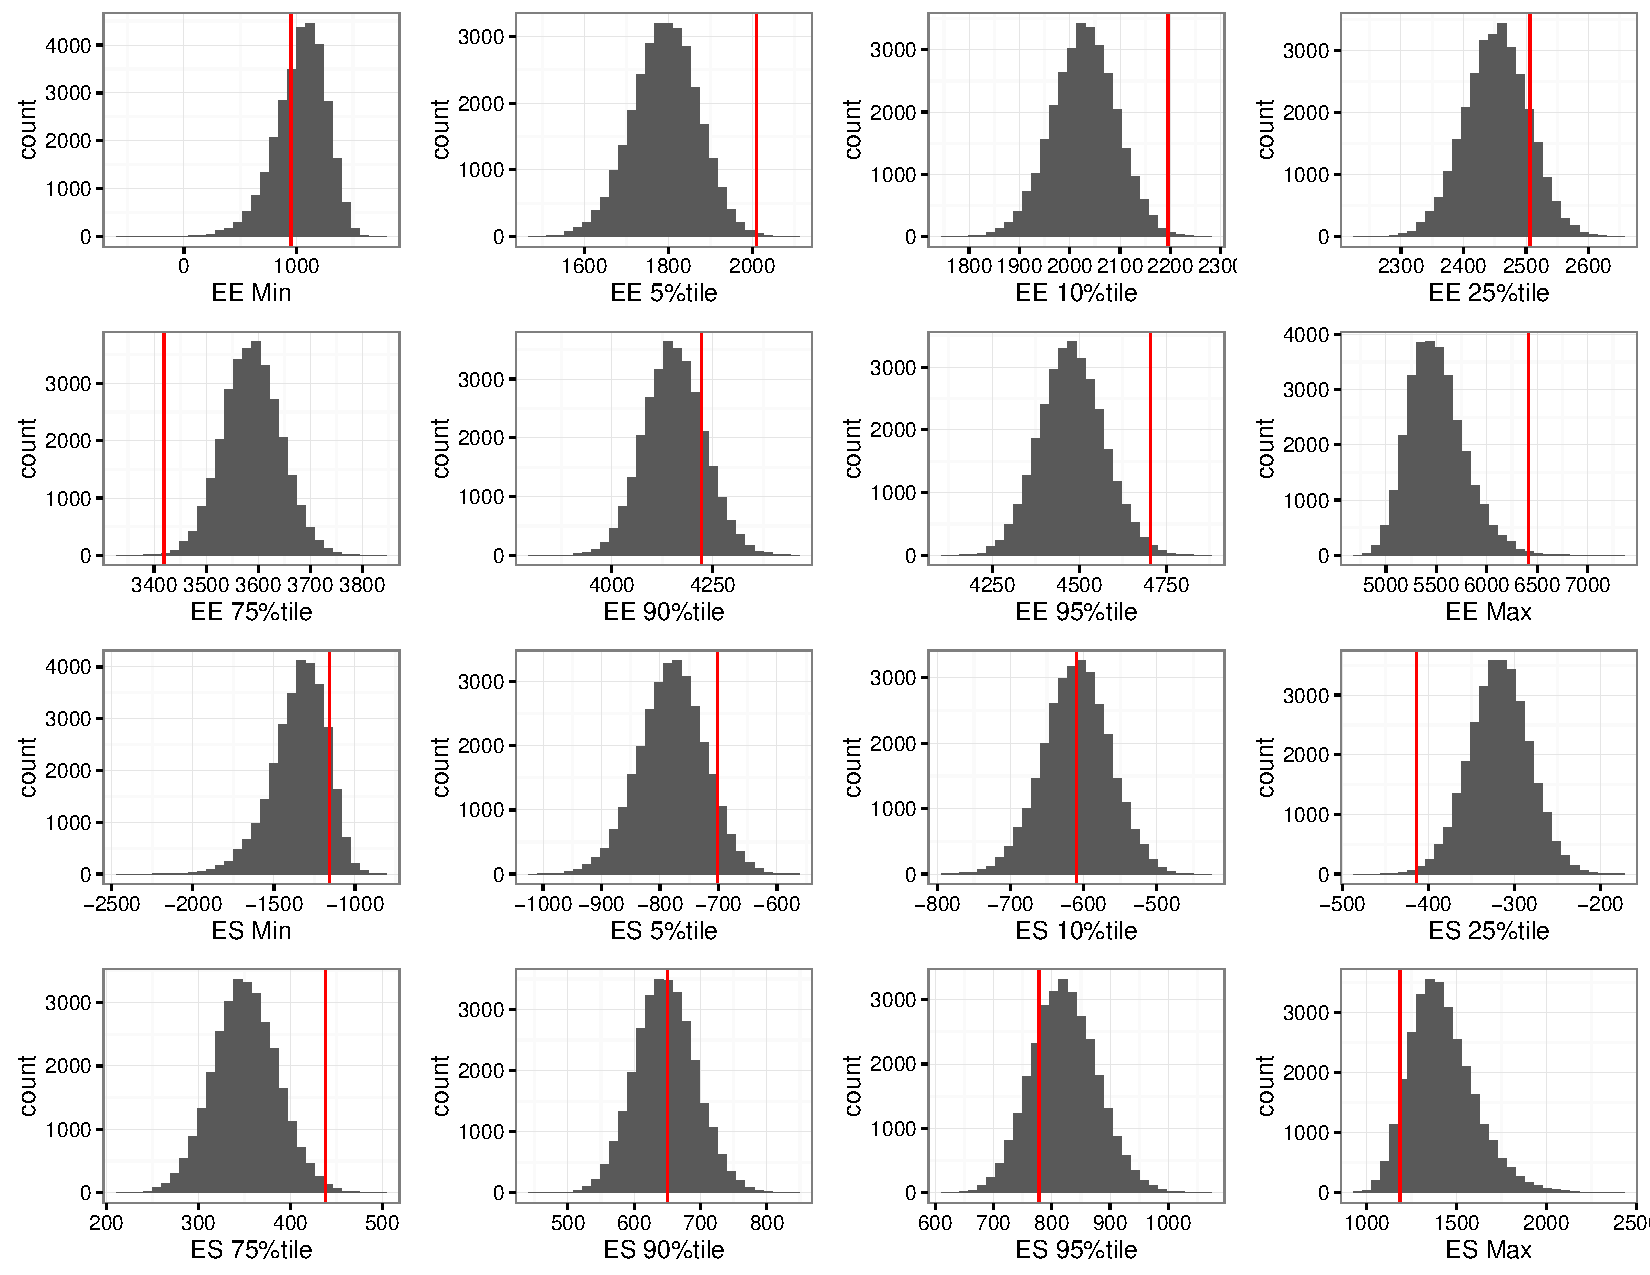
\includegraphics[width=17cm,height=15cm]{manual_figure/wpydiag1.pdf}
%   \caption{Posterior Predictive Discrepancy Measures For $Y^{EE}$ and $Y^{\Delta ES}$ for Model 1 with Normal Errors}
%   \label{wpydiag1}
%   \end{figure}
% 
% 
%  %post pred check for X
%  \begin{figure}
%   \centering
%   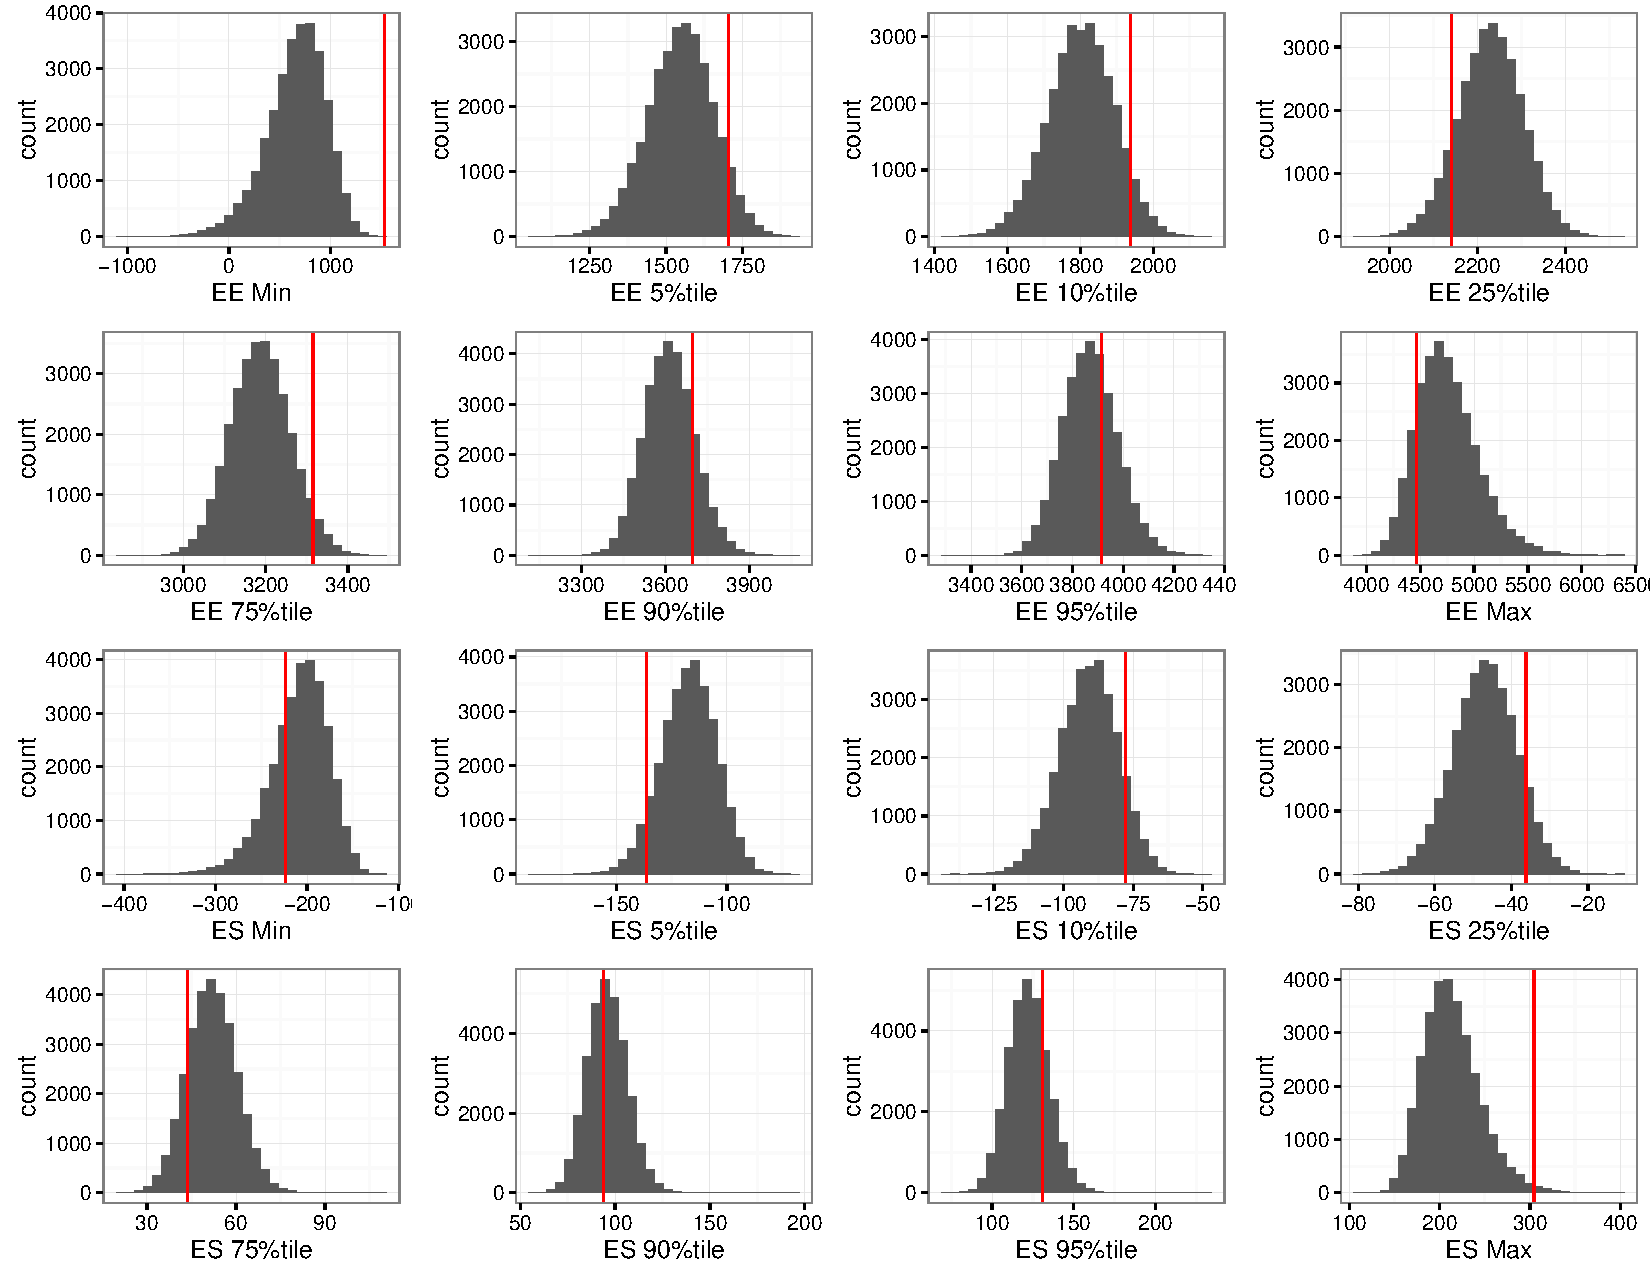
\includegraphics[width=17cm,height=15cm]{manual_figure/wpxdiag1s.pdf}
%   \caption{Posterior Predictive Discrepancy Measures For $X^{EE}$ and $X^{\Delta ES}$ for Model 1 with Skewed Normal Errors}
%   \label{wpxdiag1s}
%   \end{figure}
%  %post pred check for W
%   \begin{figure}
%   \centering
%   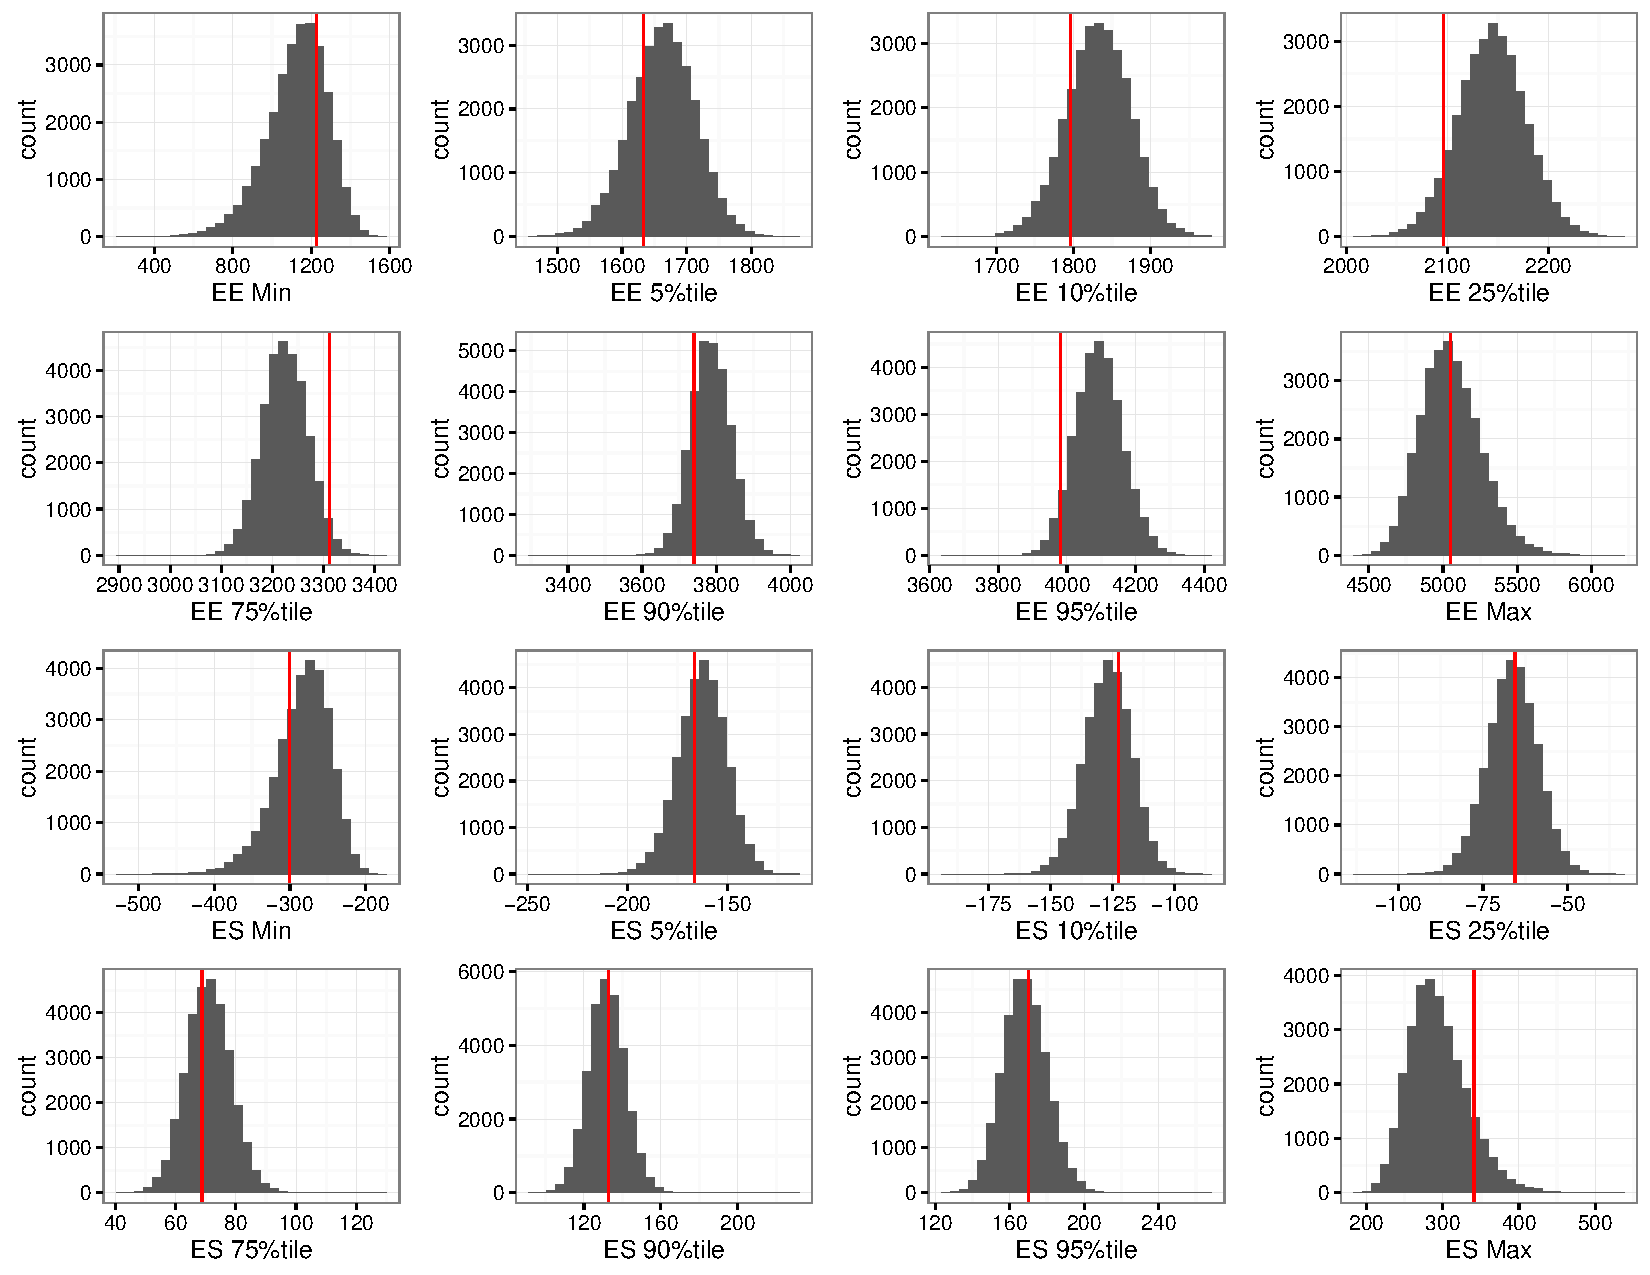
\includegraphics[width=17cm,height=15cm]{manual_figure/wpwdiag1s.pdf}
%   \caption{Posterior Predictive Discrepancy Measures For $W^{EE}$ and $W^{\Delta ES}$ for Model 1 with Skewed Normal Errors}
%   \label{wpwdiag1s}
%   \end{figure}
%  %post pred check for Y
%   \begin{figure}
%   \centering
%   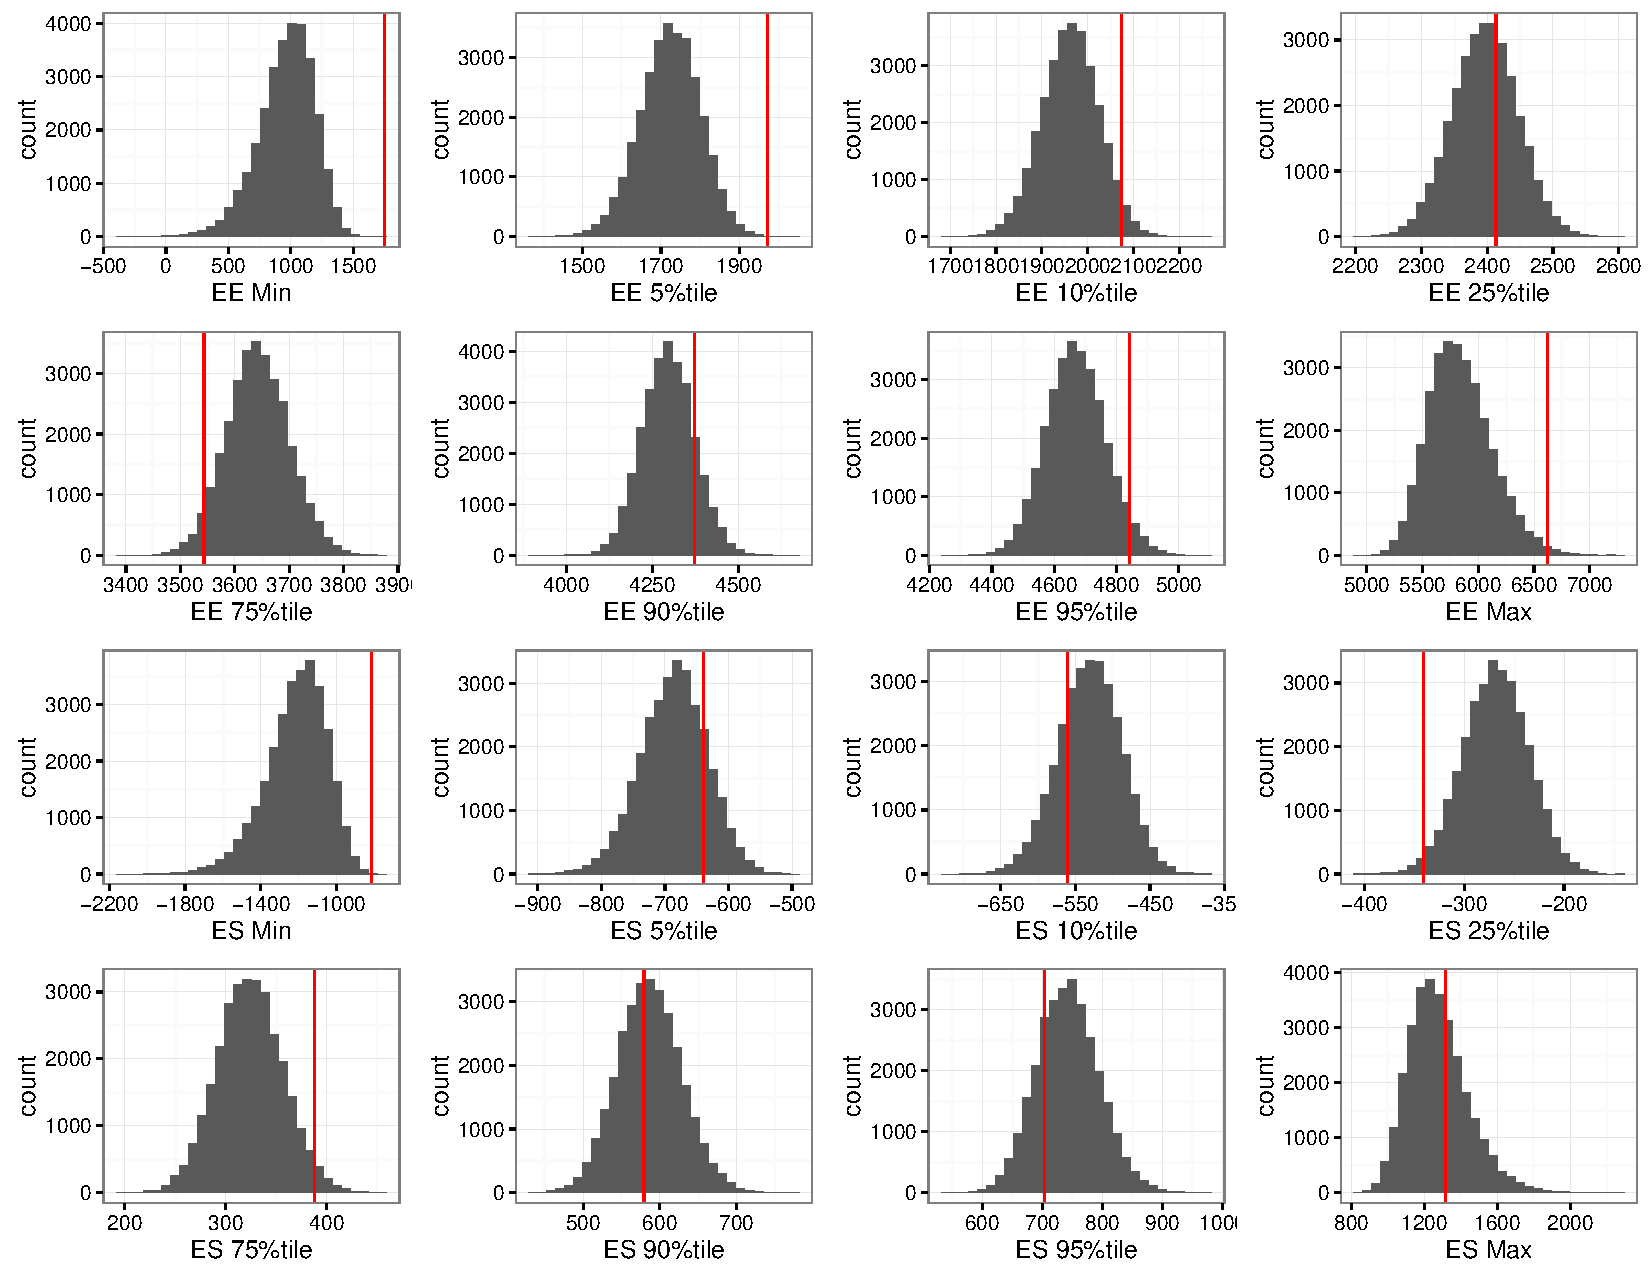
\includegraphics[width=17cm,height=15cm]{manual_figure/wpydiag1s.pdf}
%   \caption{Posterior Predictive Discrepancy Measures For $Y^{EE}$ and $Y^{\Delta ES}$ for Model 1 with Skewed Normal Errors}
%   \label{wpydiag1s}
%   \end{figure}
% 
% 
%  %post pred check for X
%  \begin{figure}
%   \centering
%   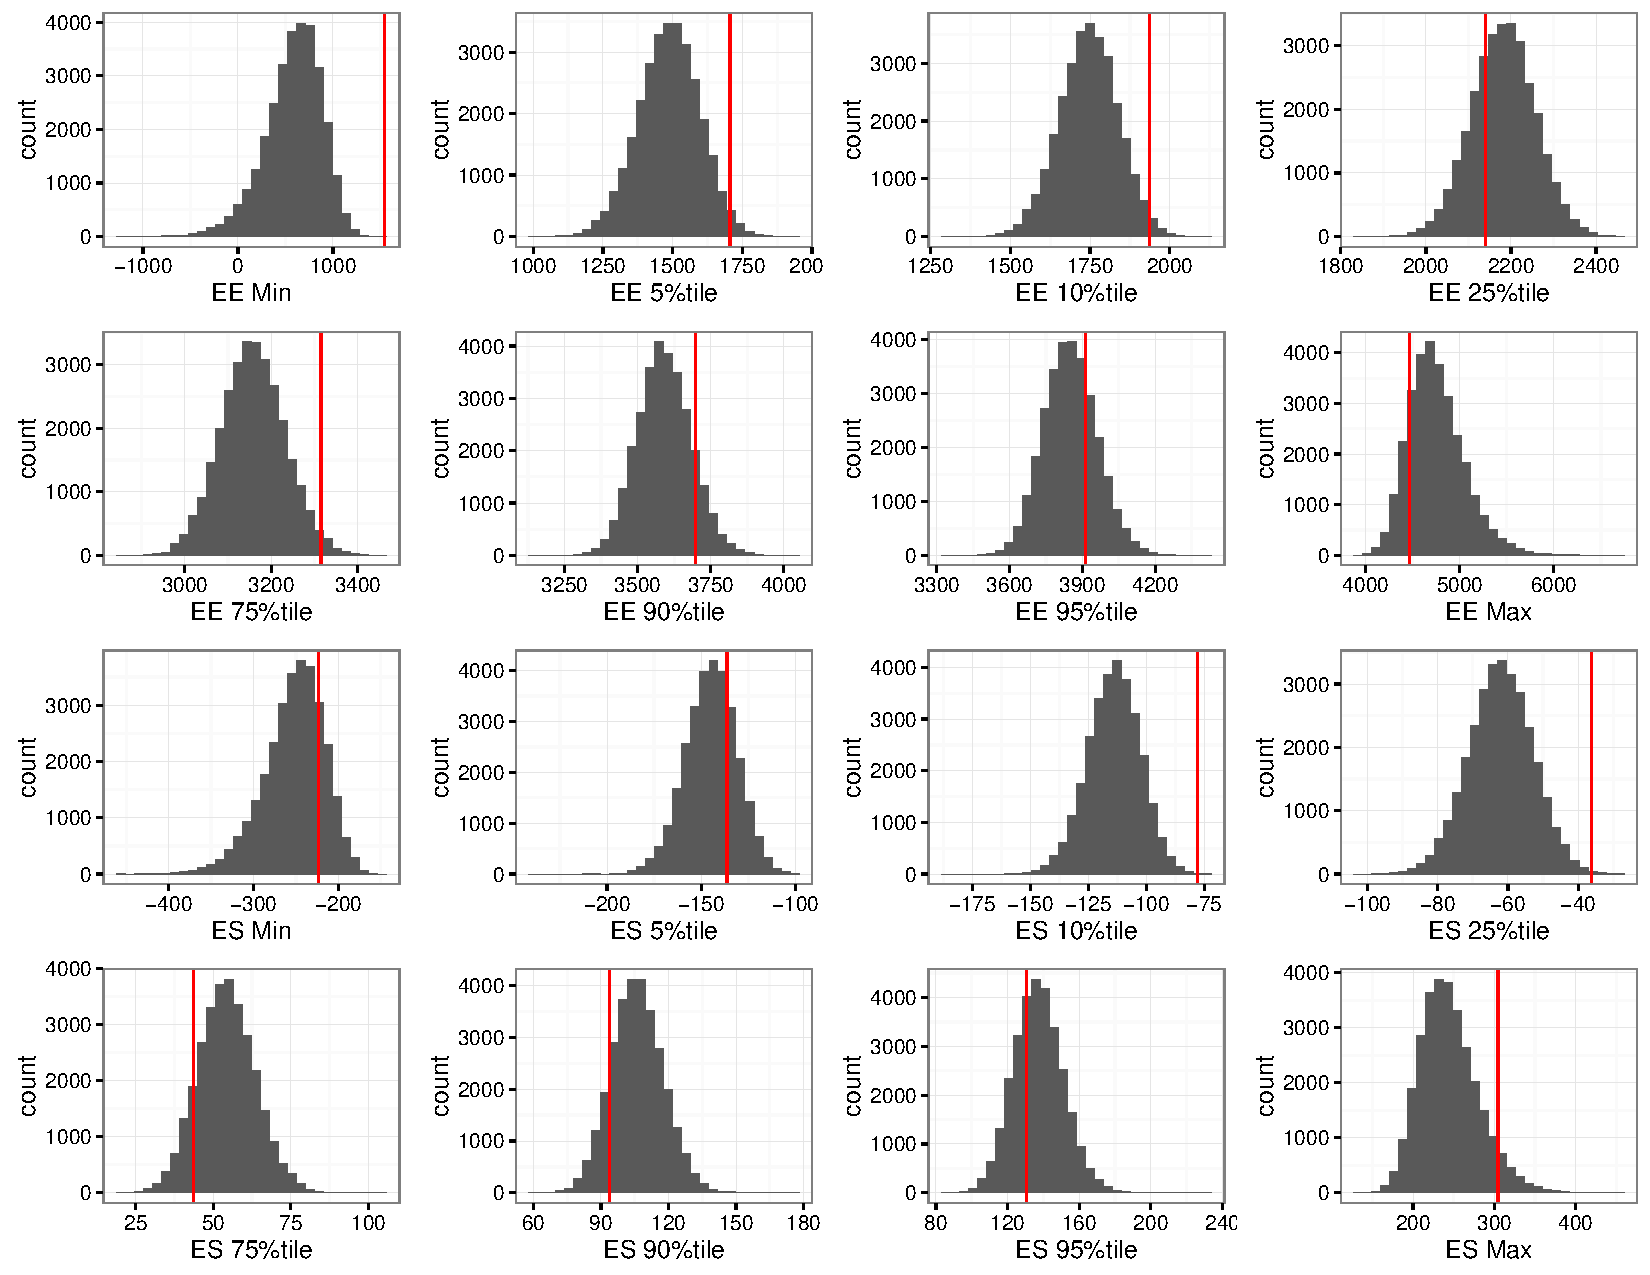
\includegraphics[width=17cm,height=15cm]{manual_figure/wpxdiag1b.pdf}
%   \caption{Posterior Predictive Discrepancy Measures For $X^{EE}$ and $X^{\Delta ES}$ for Model 1 with Bimodal  Errors}
%   \label{wpxdiag1b}
%   \end{figure}
%  %post pred check for W
%   \begin{figure}
%   \centering
%   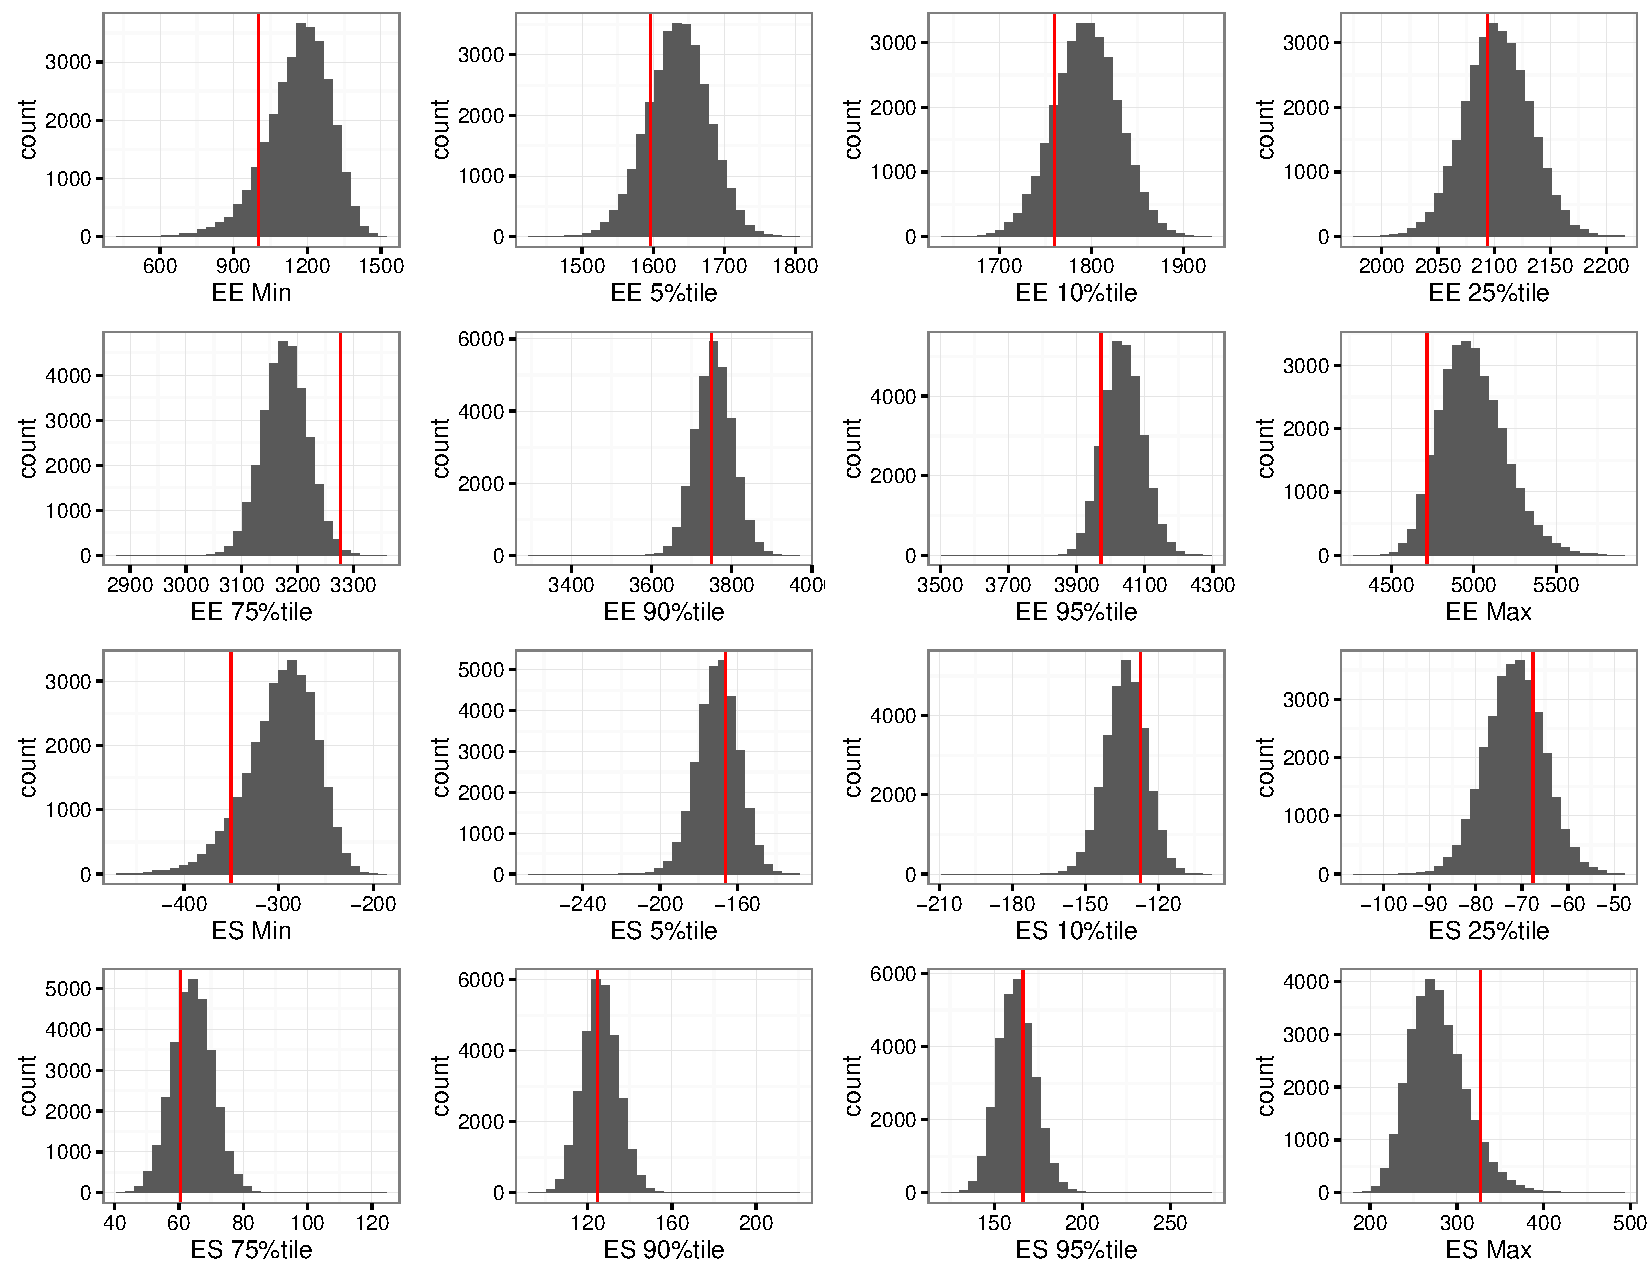
\includegraphics[width=17cm,height=15cm]{manual_figure/wpwdiag1b.pdf}
%   \caption{Posterior Predictive Discrepancy Measures For $W^{EE}$ and $W^{\Delta ES}$ for Model 1 with Bimodal Errors}
%   \label{wpwdiag1b}
%   \end{figure}
%  %post pred check for Y
%   \begin{figure}
%   \centering
%   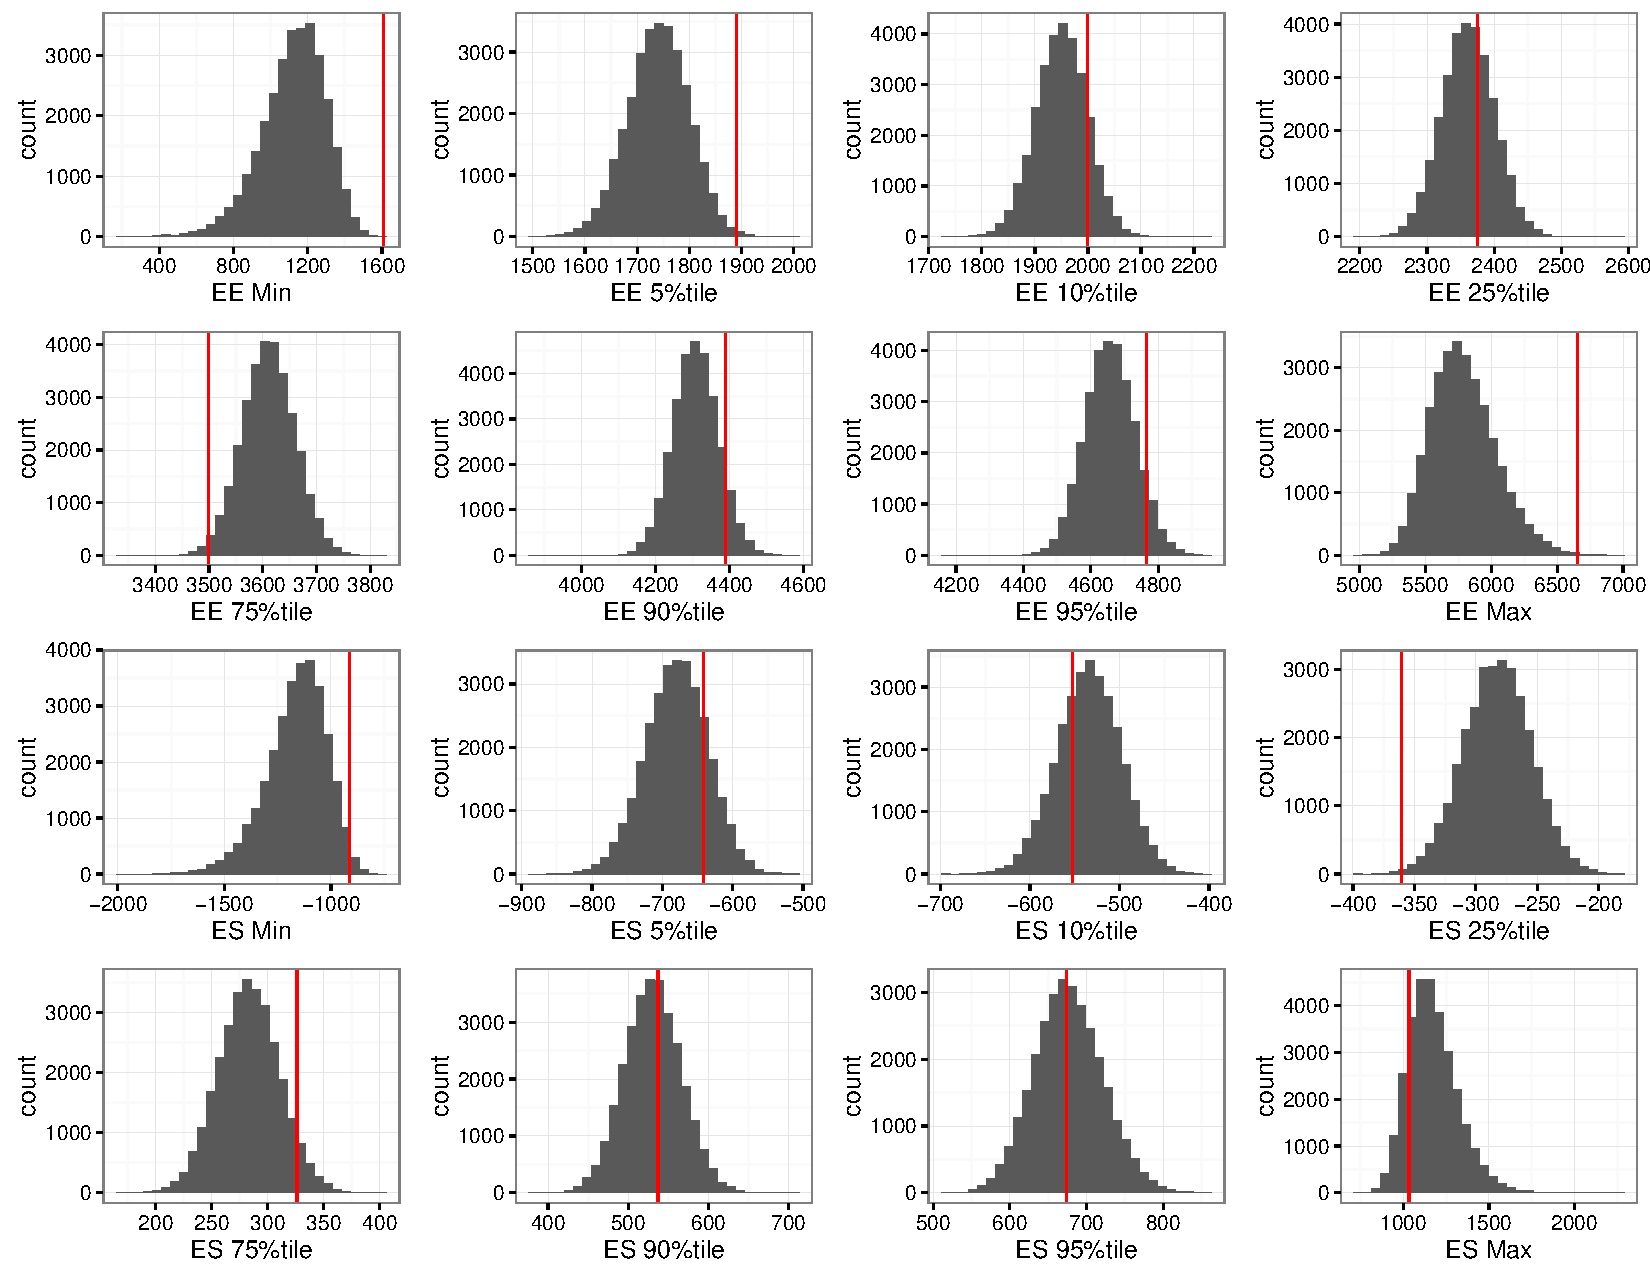
\includegraphics[width=17cm,height=15cm]{manual_figure/wpydiag1b.pdf}
%   \caption{Posterior Predictive Discrepancy Measures For $Y^{EE}$ and $Y^{\Delta ES}$ for Model 1 with Bimodal Errors}
%   \label{wpydiag1b}
%   \end{figure}
%--------------------------------%
% \subsection{Model BVN}
% %----------------------------------%
% % 
% We didn't explicitly introduce Model BVN before, but it is the same as Model DP except we assume a bivariate normal distribution for the latent variables $(X_i^{EE},X_i^{\Delta ES})$ instead of the Dirichlet Process. This is a simplifying assumption that we will justify in the next subsection. Tables \ref{mbvnwpestimates}, \ref{mbvnswpestimates}, \ref{mbvnbwpestimates} give posterior quantiles for this model under normal, skewed, and bimodal errors respectively. Quantiles for data under normal and skewed data look similar, while parameter estimates vary more when looking at bimodal errors. This is similar to what happened in previous models. 
% 
% Figures \ref{wpxdiagbvn}, \ref{wpxdiagbvns}, \ref{wpxdiagbvnb} show plots of posterior predictive assessment for the latent variables under normal, skewed, and bimodal errors respectively. Under normal and skewed errors, these don't look too bad except for one or two truths not being covered well. The bimodal errors show some more problems on the $\Delta$ES side in particular. 
% 
% Figures \ref{wpwdiagbvn}, \ref{wpwdiagbvns}, \ref{wpwdiagbvnb} show the same plots except for gold standard measurements. The assessments for the normal errors look good as  these are under correct specification. Even under skewed or bimodal errors, there doesn't seem to be any glaring issues. Figures \ref{wpydiagbvn}, \ref{wpydiagbvns}, \ref{wpydiagbvnb} show the same plots except for cheap measurements. As with the gold standard measurements, there doesn't appear to be any issues in these assessment plots. This gives some confidence in an amount of robustness to misspecification of measurement error distribution.
% 
% 
% Table \ref{pmse2} gives PMSE for both the EE and $\Delta$ES regression functions under normal, skewed, and bimodal errors. Not only does ignoring the measurement error give bad parameter estimates and posterior predictive checks, but also its prediction is poor. Our model that has splines in its regression function  whose knots can varry iteration to iteration performs much better than just a linear model. 
% 
% \begin{table}[ht]
% \centering
% \begin{tabular}{rrrrrr|r}
%   \hline
%  & 2.5\% & 25\% & 50\% & 75\% & 97.5\% & Truth\\
%   \hline
% $\mu_x^{EE}$ & 2610.19 & 2663.99 & 2691.59 & 2719.67 & 2772.07 \\ 
%   $\mu_x^{\Delta ES}$ & -8.11 & -1.42 & 2.08 & 5.61 & 12.38 \\ 
%   $\sigma_{yee}$ & 381.01 & 396.92 & 405.71 & 414.93 & 435.80 \\ 
%   $\sigma_{yes}$ & 296.81 & 309.75 & 316.87 & 324.23 & 339.56 \\ 
%   $\sigma_{wee}$ & 236.55 & 248.84 & 255.74 & 262.91 & 277.50 & 250\\ 
%   $\sigma_{wes}$ & 64.41 & 67.17 & 68.73 & 70.33 & 73.51 & 72.86\\ 
%   $\sigma_{xee}$ & 637.76 & 673.81 & 694.27 & 715.80 & 759.92 \\ 
%   $\sigma_{xes}$ & 67.03 & 72.23 & 75.17 & 78.12 & 84.09 \\ 
%   $\rho$ & -0.23 & -0.15 & -0.11 & -0.06 & 0.02 \\ 
%   $\gamma_{1,ee}$ & 178.48 & 244.17 & 278.90 & 314.08 & 382.01 & 300\\ 
%   $\gamma_{2,ee}$ & -0.05 & 4.81 & 7.34 & 9.87 & 14.70 & 14\\ 
%   $\gamma_{3,ee}$ & -17.51 & -13.32 & -11.09 & -8.84 & -4.59 & -7\\ 
%   $\gamma_{1,es}$ & -296.12 & -241.05 & -212.36 & -183.20 & -126.47 & -200 \\ 
%   $\gamma_{2,es}$ & 3.02 & 6.97 & 9.05 & 11.17 & 15.32 & 8\\ 
%   $\gamma_{3,es}$ & -10.58 & -6.88 & -4.94 & -3.05 & 0.63 & -5\\ 
%   \hline
% \end{tabular}
% \caption{Parameter estimates for Model BVN for Normal errors with correct specification of within person errors}
% \label{mbvnwpestimates}
% \end{table}
% 
% 
% \begin{table}[ht]
% \centering
% \begin{tabular}{rrrrrr|r}
%   \hline
%  & 2.5\% & 25\% & 50\% & 75\% & 97.5\% & Truth\\
%   \hline
% $\mu_x^{EE}$ & 2622.55 & 2675.43 & 2703.64 & 2732.01 & 2786.64 \\ 
%   $\mu_x^{\Delta ES}$ & -7.62 & -0.93 & 2.59 & 6.10 & 12.84 \\ 
%   $\sigma_{yee}$ & 371.38 & 387.03 & 395.75 & 405.05 & 425.11 \\ 
%   $\sigma_{yes}$ & 291.18 & 303.53 & 310.39 & 317.55 & 331.87 \\ 
%   $\sigma_{wee}$ & 241.21 & 253.60 & 260.49 & 267.51 & 281.58 & 250 \\ 
%   $\sigma_{wes}$ & 65.05 & 67.98 & 69.56 & 71.24 & 74.65 & 72.862\\ 
%   $\sigma_{xee}$ & 641.81 & 679.00 & 699.07 & 720.28 & 764.17 \\ 
%   $\sigma_{xes}$ & 65.68 & 70.97 & 73.92 & 76.89 & 82.68 \\ 
%   $\rho$ & -0.28 & -0.20 & -0.15 & -0.11 & -0.02 \\ 
%   $\gamma_{1,ee}$ & 150.70 & 216.27 & 251.30 & 285.24 & 352.67 & 300 \\ 
%   $\gamma_{2,ee}$ & 0.29 & 5.23 & 7.76 & 10.27 & 15.22 & 14\\ 
%   $\gamma_{3,ee}$ & -17.58 & -13.31 & -11.06 & -8.85 & -4.57 & -7 \\ 
%   $\gamma_{1,es}$ & -297.09 & -244.54 & -217.35 & -190.06 & -138.10 & -200 \\ 
%   $\gamma_{2,es}$ & 2.31 & 6.06 & 8.01 & 9.99 & 13.75 & 8\\ 
%   $\gamma_{3,es}$ & -9.18 & -5.74 & -3.93 & -2.15 & 1.27 & -5 \\ 
%    \hline
% \end{tabular}
% \caption{Parameter estimates for Model BVN for Skewed errors with correct specification of within person errors}
% \label{mbvnswpestimates}
% \end{table}
% 
% \begin{table}[ht]
% \centering
% \begin{tabular}{rrrrrr|r}
%   \hline
%  & 2.5\% & 25\% & 50\% & 75\% & 97.5\% & Truth \\
%   \hline
% $\mu_x^{EE}$ & 2581.07 & 2634.84 & 2662.65 & 2690.48 & 2743.29 \\ 
%   $\mu_x^{\Delta ES}$ & -14.55 & -7.47 & -3.70 & 0.01 & 6.92 \\ 
%   $\sigma_{yee}$ & 245.77 & 261.27 & 269.43 & 277.84 & 297.13 \\ 
%   $\sigma_{yes}$ & 223.45 & 232.56 & 237.53 & 242.90 & 253.34 \\ 
%   $\sigma_{wee}$ & 176.09 & 186.78 & 192.79 & 199.36 & 213.55 & 250\\ 
%   $\sigma_{wes}$ & 48.83 & 50.96 & 52.15 & 53.36 & 55.79 & 72.862 \\ 
%   $\sigma_{xee}$ & 646.03 & 682.15 & 702.09 & 722.74 & 764.86 \\ 
%   $\sigma_{xes}$ & 79.09 & 84.14 & 86.92 & 89.80 & 95.74 \\ 
%   $\rho$ & -0.06 & 0.02 & 0.06 & 0.10 & 0.18 \\ 
%   $\gamma_{1,ee}$ & 125.13 & 175.72 & 201.12 & 226.66 & 276.14 & 300 \\ 
%   $\gamma_{2,ee}$ & 4.54 & 8.05 & 9.86 & 11.66 & 15.18 & 14\\ 
%   $\gamma_{3,ee}$ & -16.95 & -13.86 & -12.24 & -10.63 & -7.58 & -7 \\ 
%   $\gamma_{1,es}$ & -239.57 & -198.67 & -177.29 & -155.91 & -115.00 & -200 \\ 
%   $\gamma_{2,es}$ & 1.66 & 4.61 & 6.19 & 7.71 & 10.72 & 8\\ 
%   $\gamma_{3,es}$ & -7.02 & -4.31 & -2.90 & -1.49 & 1.20 & -5\\ 
%    \hline
% \end{tabular}
% \caption{Parameter estimates for Model BVN for Bimodal errors with correct specification of within person errors}
% \label{mbvnbwpestimates}
% \end{table}
% 
% %  %post pred check for X
%  \begin{figure}
%   \centering
%   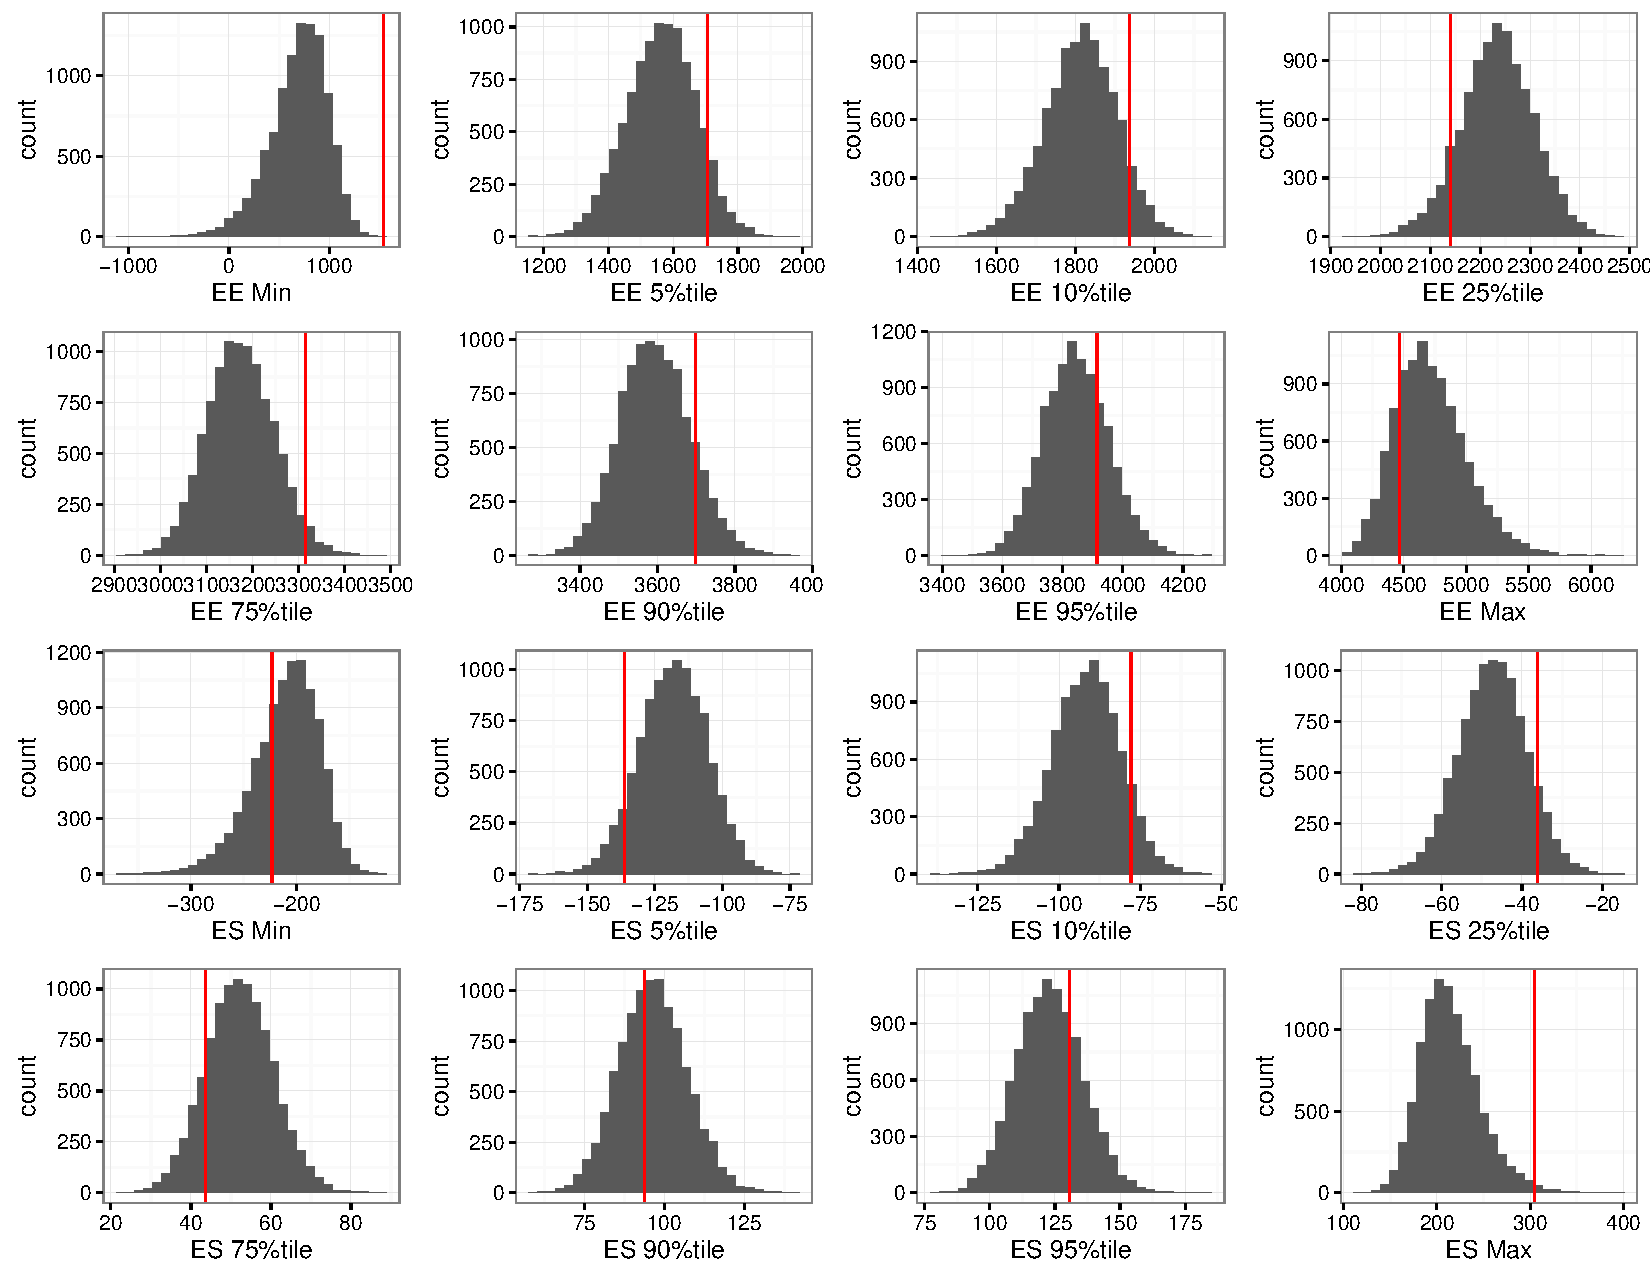
\includegraphics[width=17cm,height=15cm]{manual_figure/wpxdiagbvn.pdf}
%   \caption{Posterior Predictive Discrepancy Measures For $X^{EE}$ and $X^{\Delta ES}$ for Model BVN with Normal Errors}
%   \label{wpxdiagbvn}
%   \end{figure}
%  %post pred check for W
%   \begin{figure}
%   \centering
%   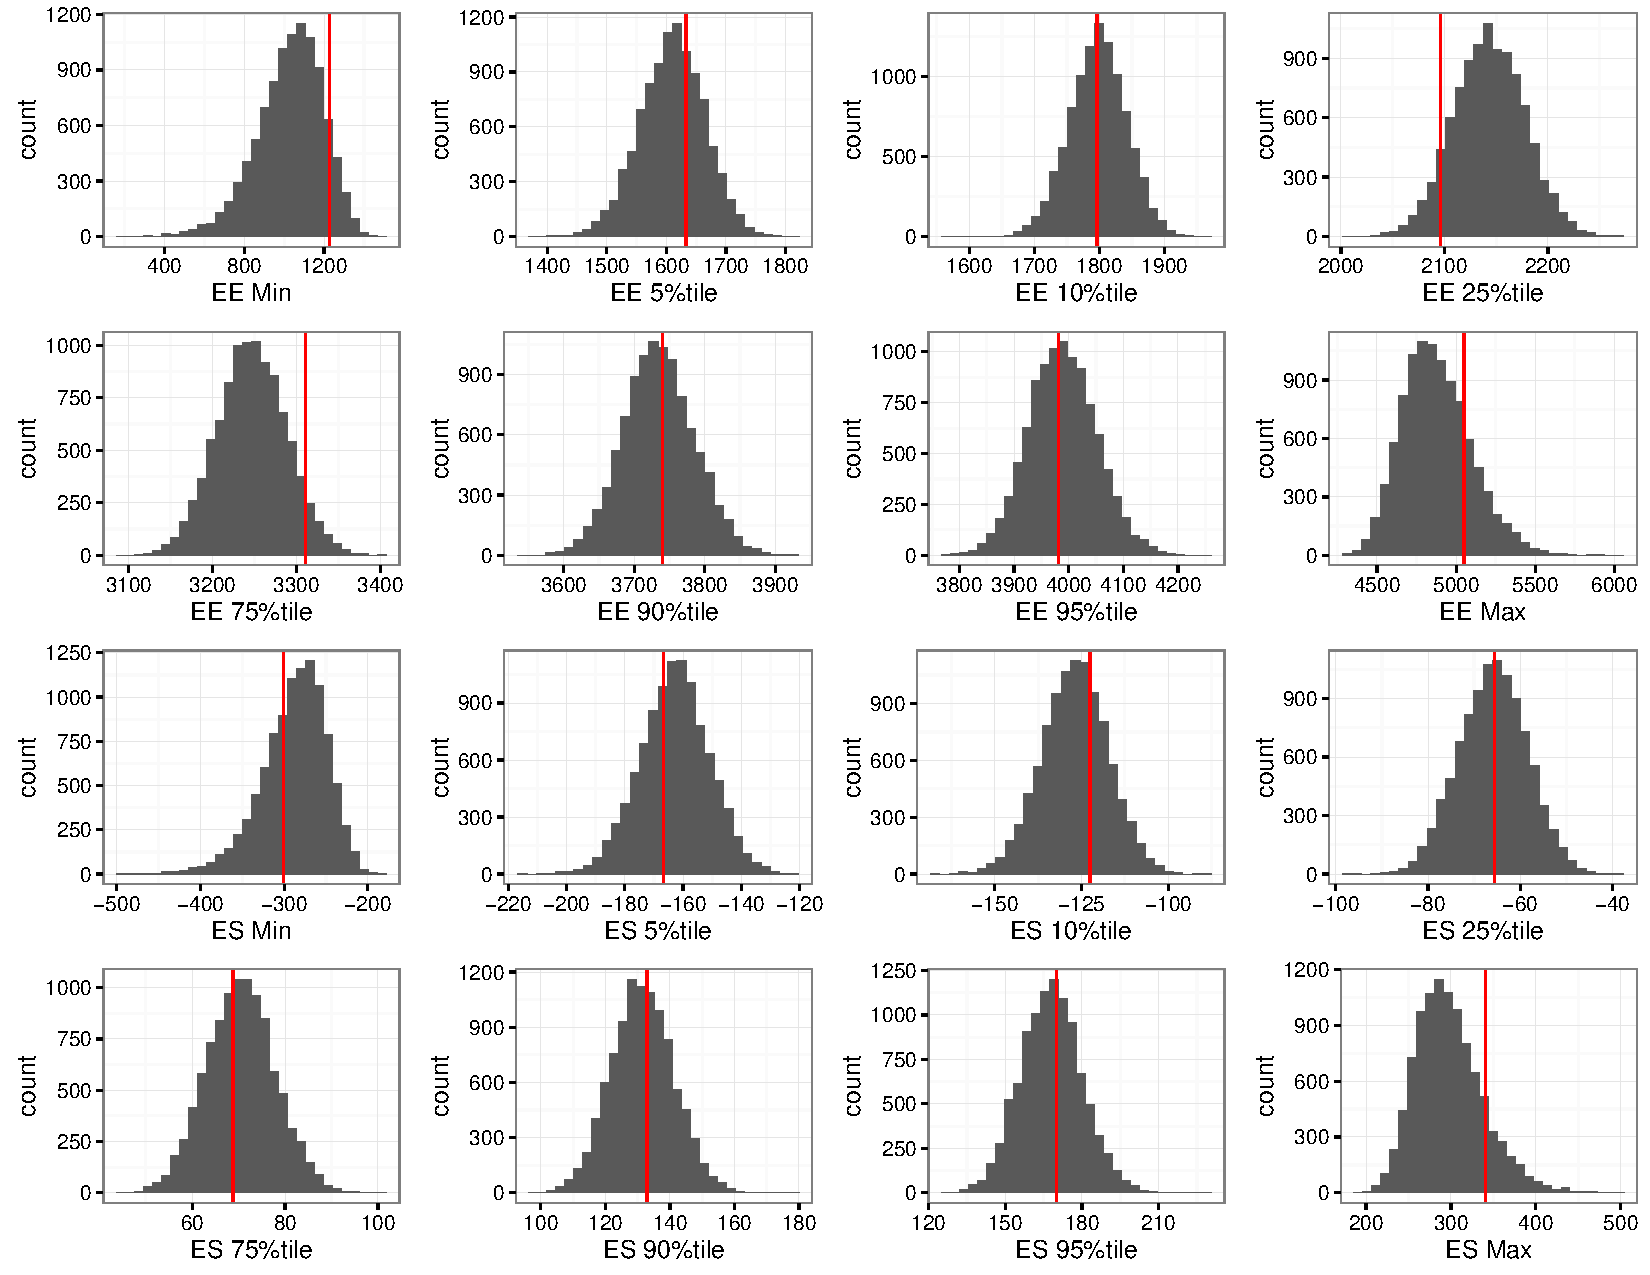
\includegraphics[width=17cm,height=15cm]{manual_figure/wpwdiagbvn.pdf}
%   \caption{Posterior Predictive Discrepancy Measures For $W^{EE}$ and $W^{\Delta ES}$ for Model BVN with Normal Errors}
%   \label{wpwdiagbvn}
%   \end{figure}
%  %post pred check for Y
%   \begin{figure}
%   \centering
%   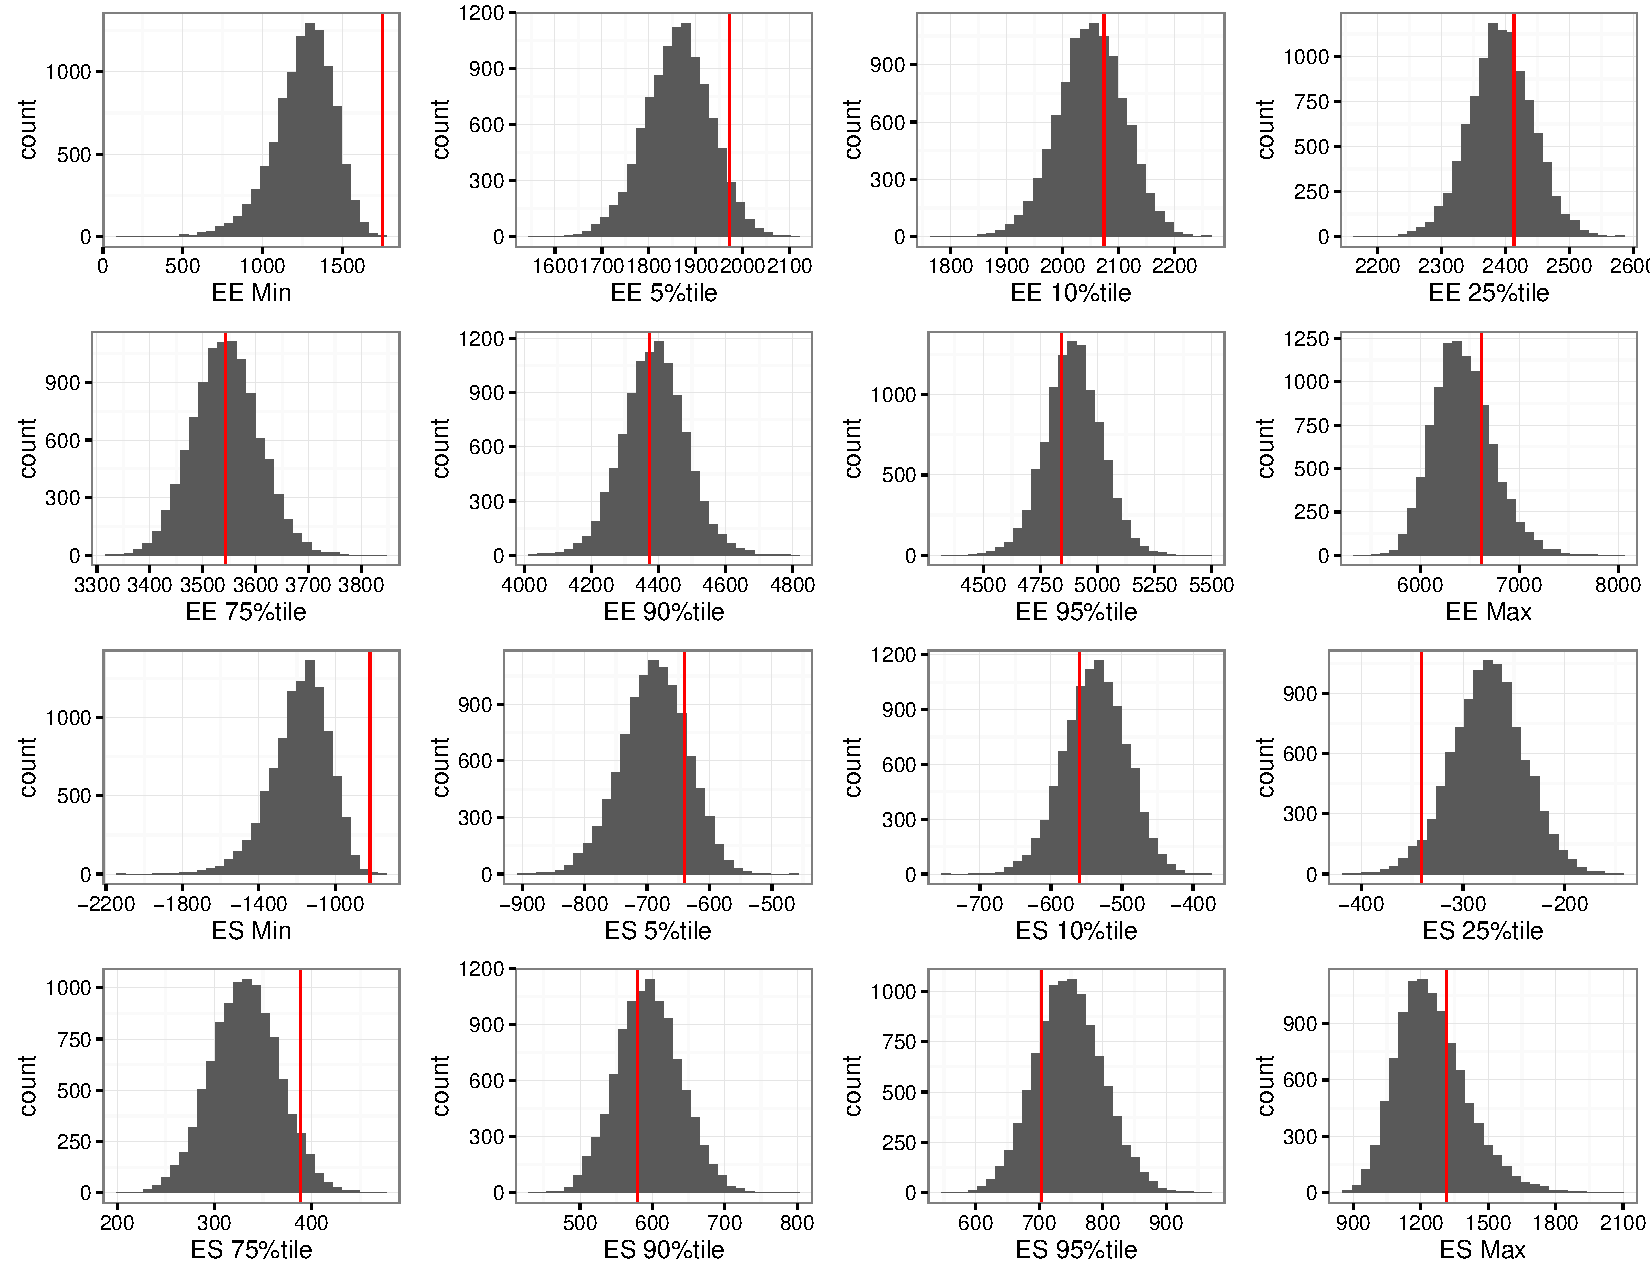
\includegraphics[width=17cm,height=15cm]{manual_figure/wpydiagbvn.pdf}
%   \caption{Posterior Predictive Discrepancy Measures For $Y^{EE}$ and $Y^{\Delta ES}$ for Model BVN with Normal Errors}
%   \label{wpydiagbvn}
%   \end{figure}
% % 
% % 
% %  %post pred check for X
%  \begin{figure}
%   \centering
%   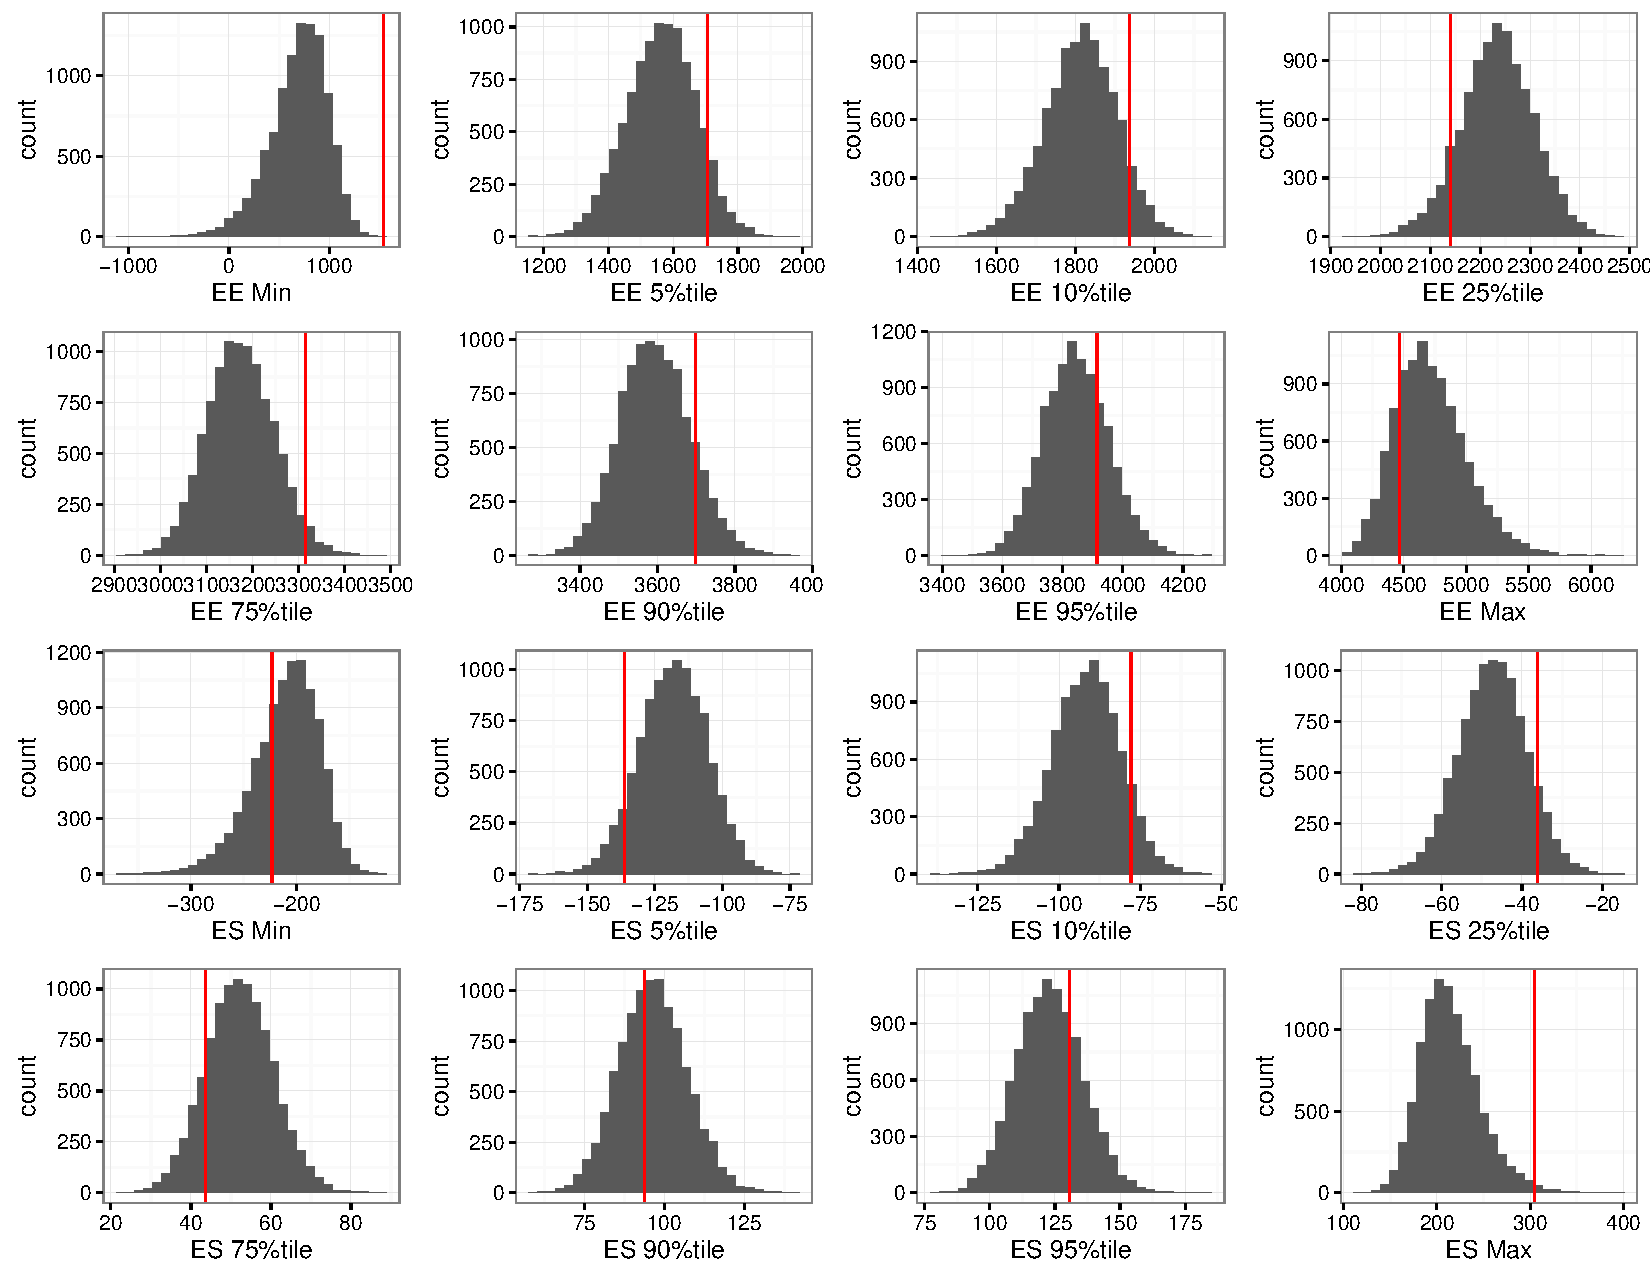
\includegraphics[width=17cm,height=15cm]{manual_figure/wpxdiagbvns.pdf}
%   \caption{Posterior Predictive Discrepancy Measures For $X^{EE}$ and $X^{\Delta ES}$ for Model BVN with Skewed Normal Errors}
%   \label{wpxdiagbvns}
%   \end{figure}
%  %post pred check for W
%   \begin{figure}
%   \centering
%   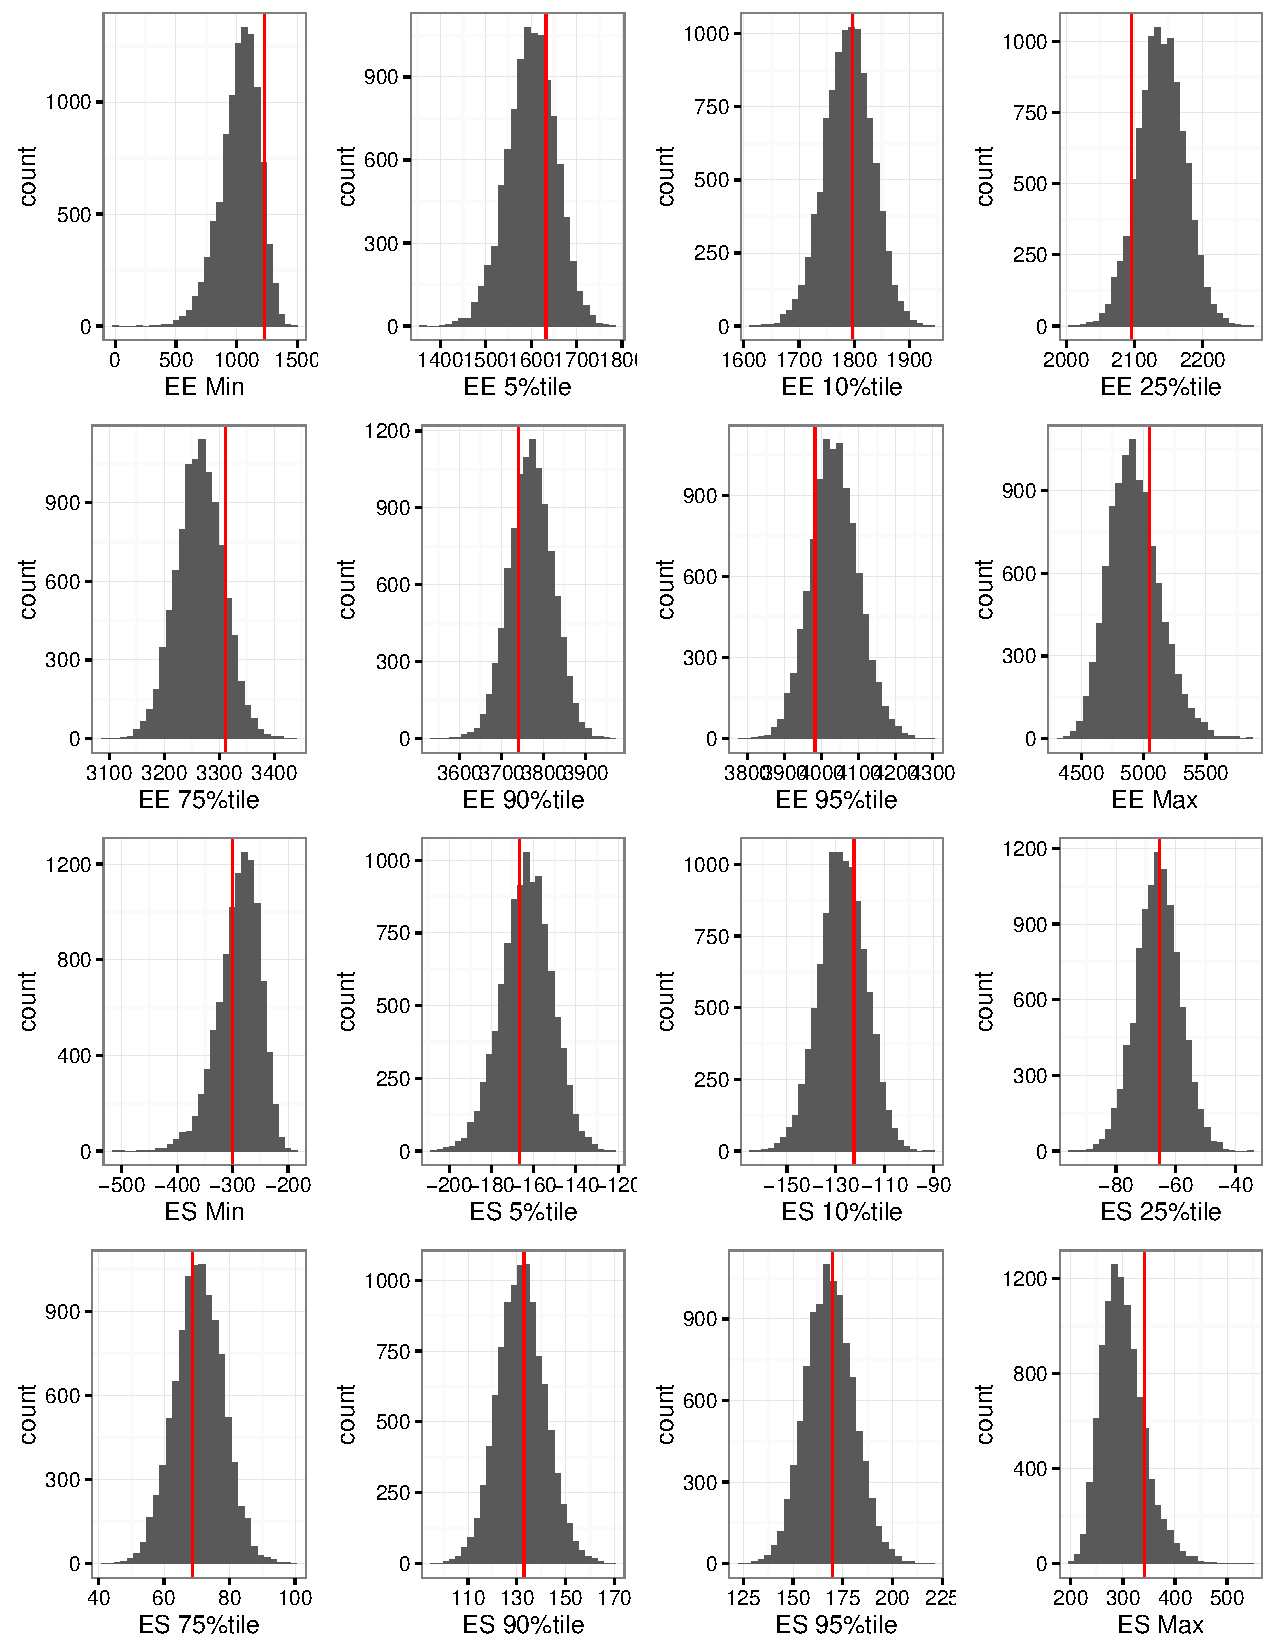
\includegraphics[width=17cm,height=15cm]{manual_figure/wpwdiagbvns.pdf}
%   \caption{Posterior Predictive Discrepancy Measures For $W^{EE}$ and $W^{\Delta ES}$ for Model BVN with Skewed Normal Errors}
%   \label{wpwdiagbvns}
%   \end{figure}
%  %post pred check for Y
%   \begin{figure}
%   \centering
%   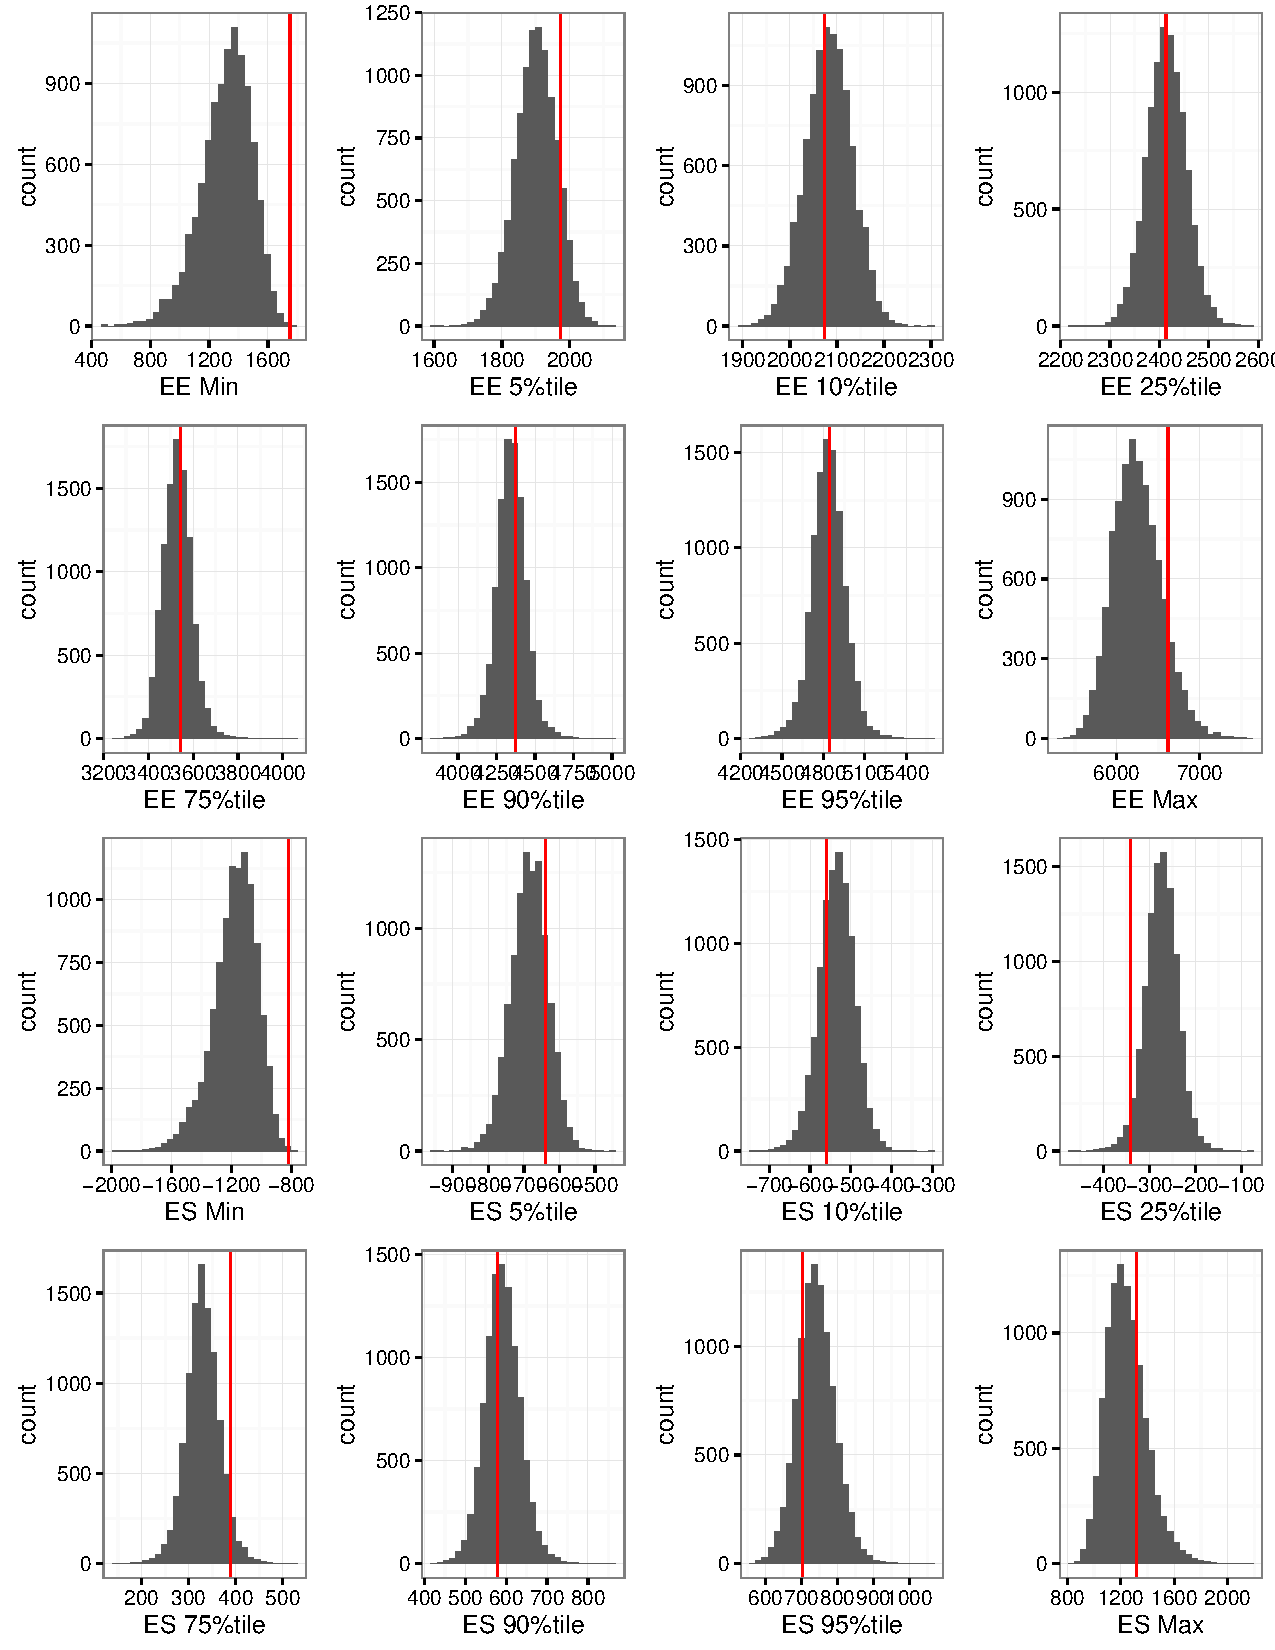
\includegraphics[width=17cm,height=15cm]{manual_figure/wpydiagbvns.pdf}
%   \caption{Posterior Predictive Discrepancy Measures For $Y^{EE}$ and $Y^{\Delta ES}$ for Model BVN with Skewed Normal Errors}
%   \label{wpydiagbvns}
%   \end{figure}
%   
%    \begin{figure}
%   \centering
%   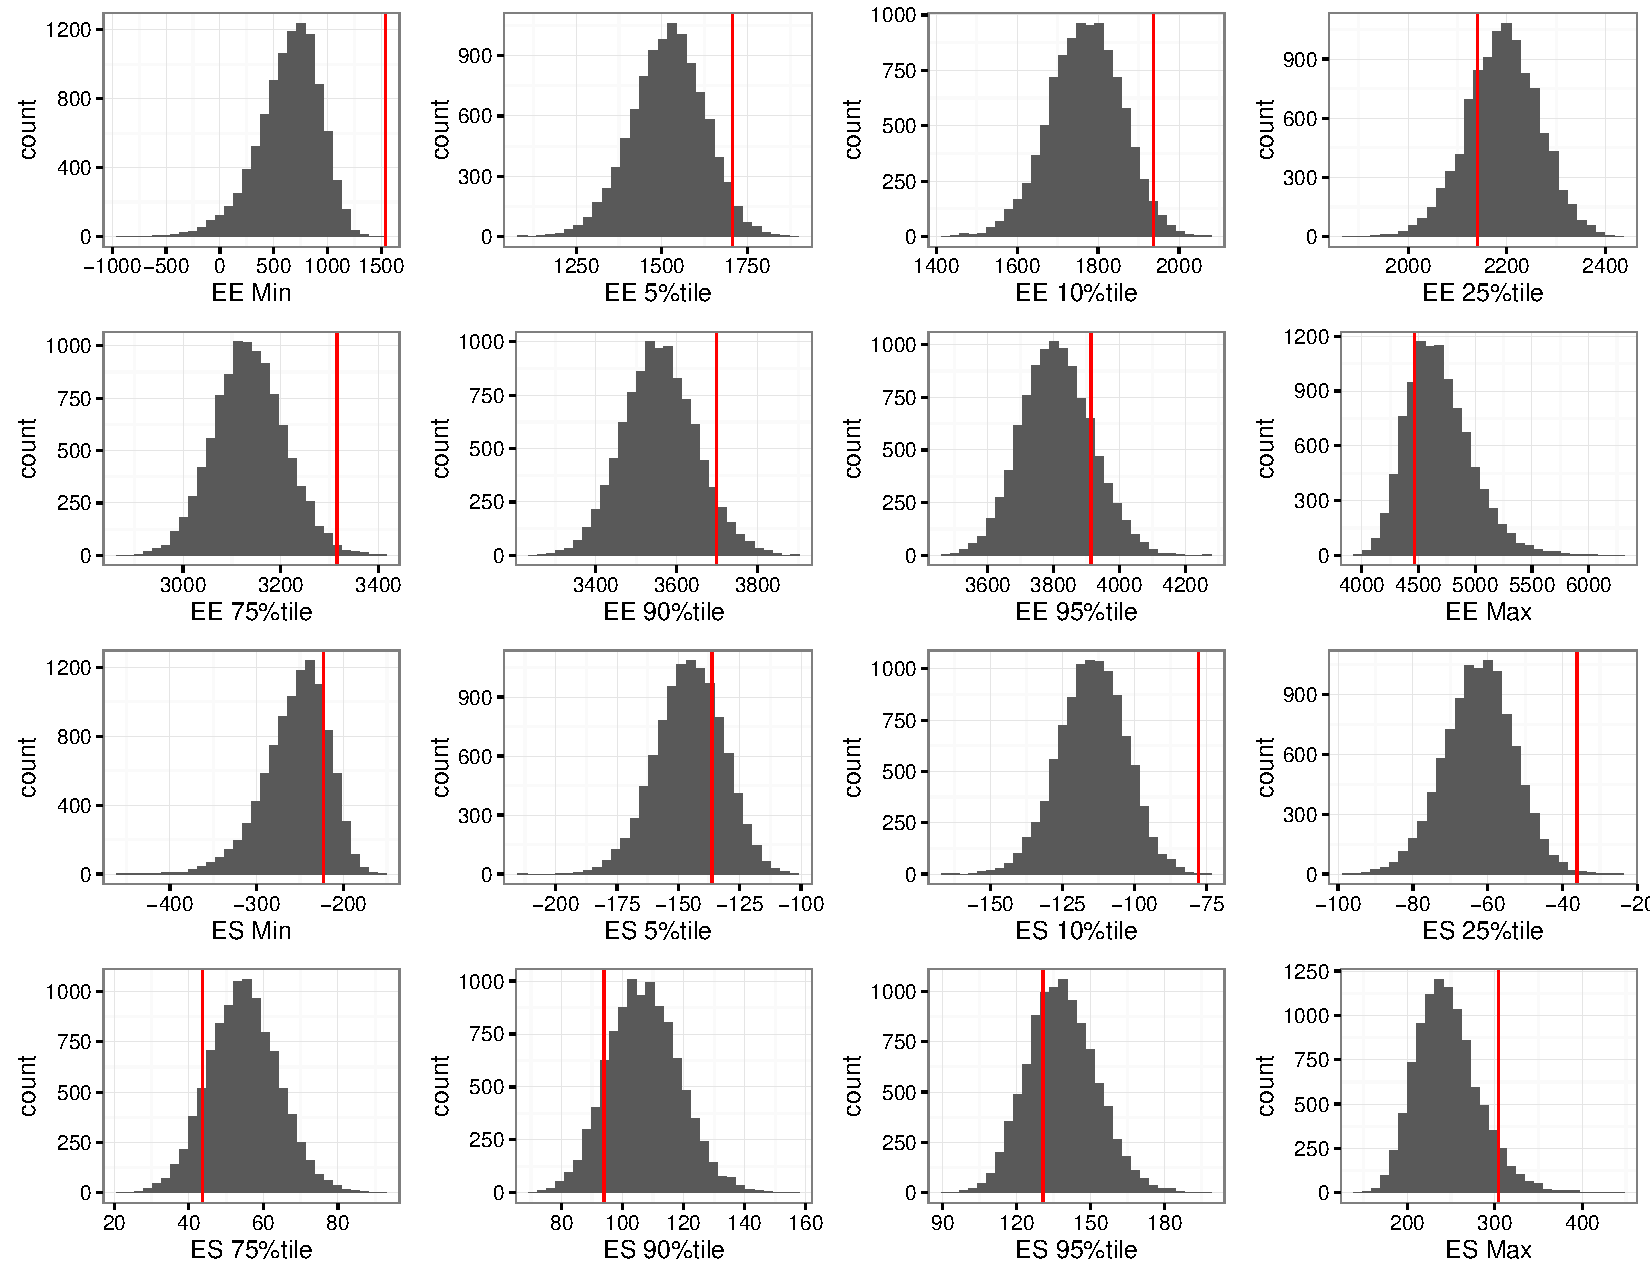
\includegraphics[width=17cm,height=15cm]{manual_figure/wpxdiagbvnb.pdf}
%   \caption{Posterior Predictive Discrepancy Measures For $X^{EE}$ and $X^{\Delta ES}$ for Model BVN with Bimodal Normal Errors}
%   \label{wpxdiagbvnb}
%   \end{figure}
%  %post pred check for W
%   \begin{figure}
%   \centering
%   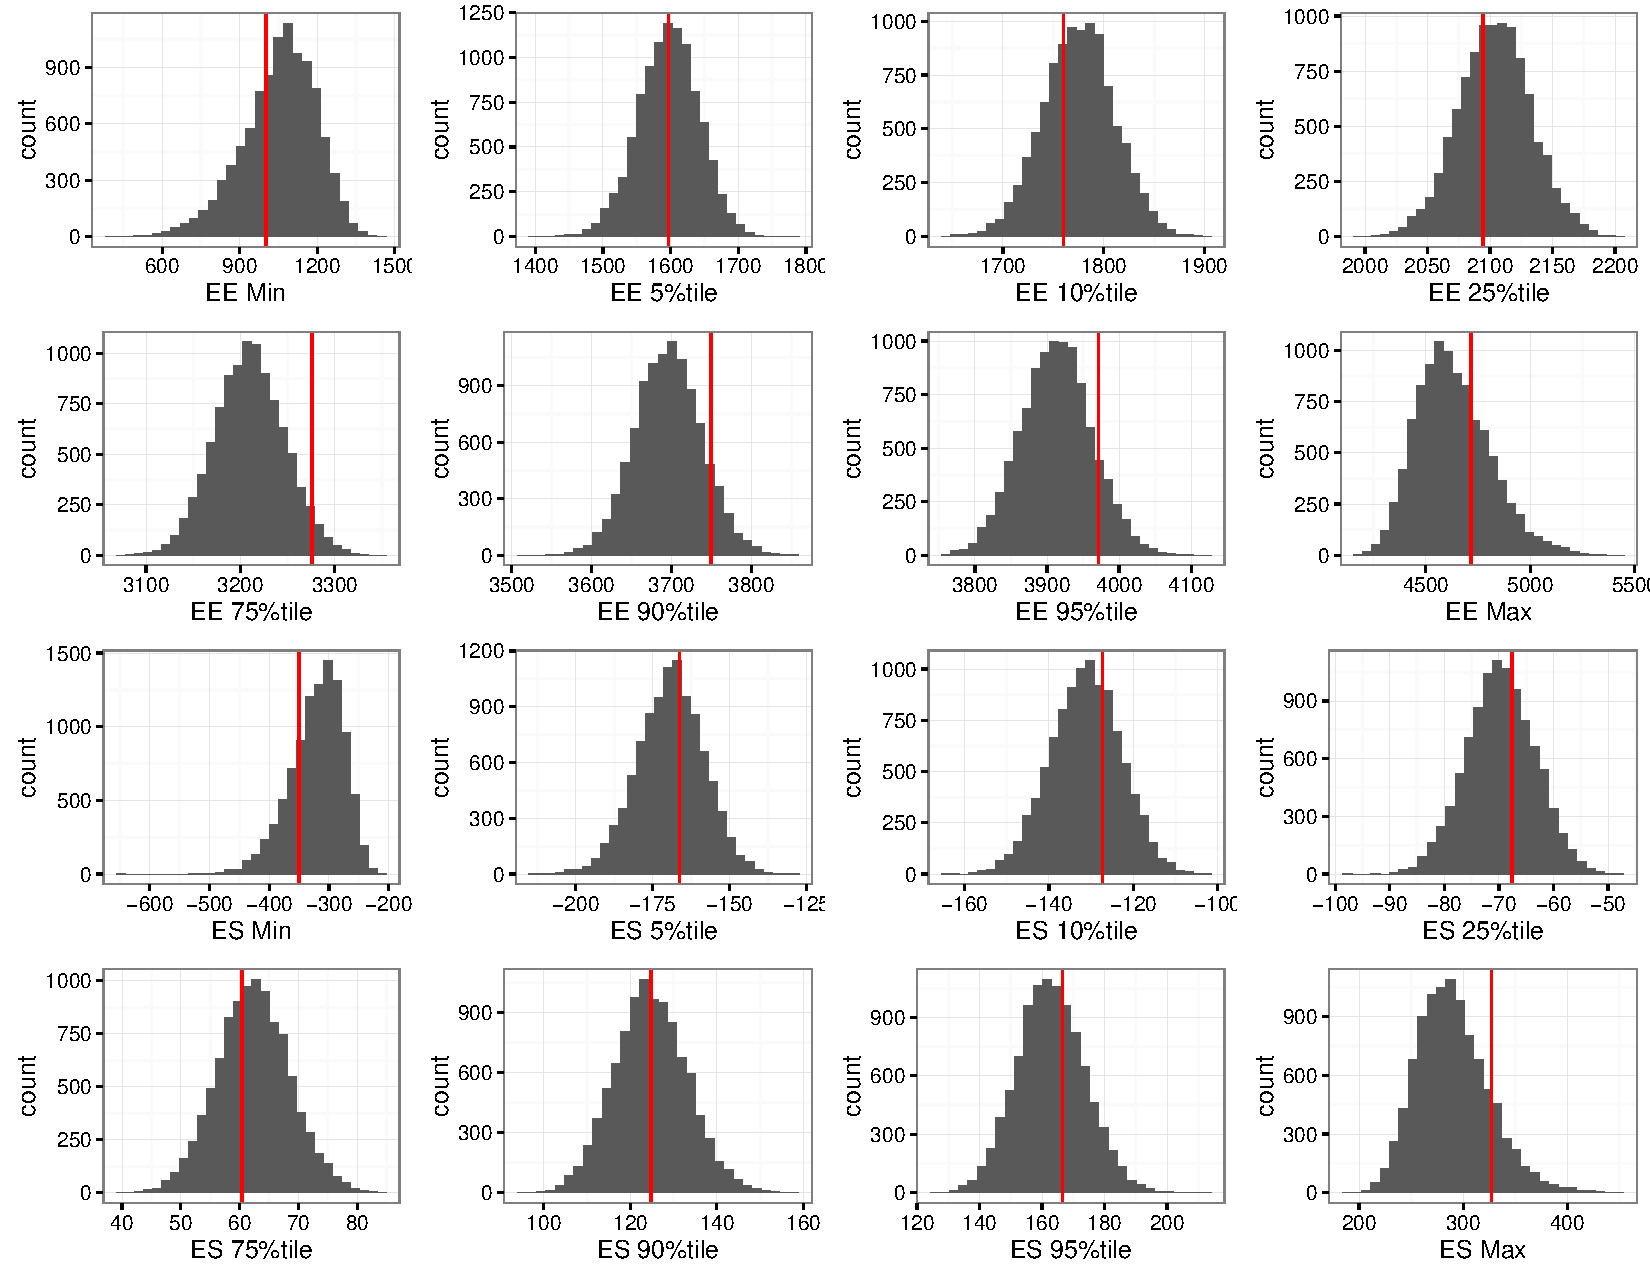
\includegraphics[width=17cm,height=15cm]{manual_figure/wpwdiagbvnb.pdf}
%   \caption{Posterior Predictive Discrepancy Measures For $W^{EE}$ and $W^{\Delta ES}$ for Model BVN with Bimodal Normal Errors}
%   \label{wpwdiagbvnb}
%   \end{figure}
%  %post pred check for Y
%   \begin{figure}
%   \centering
%   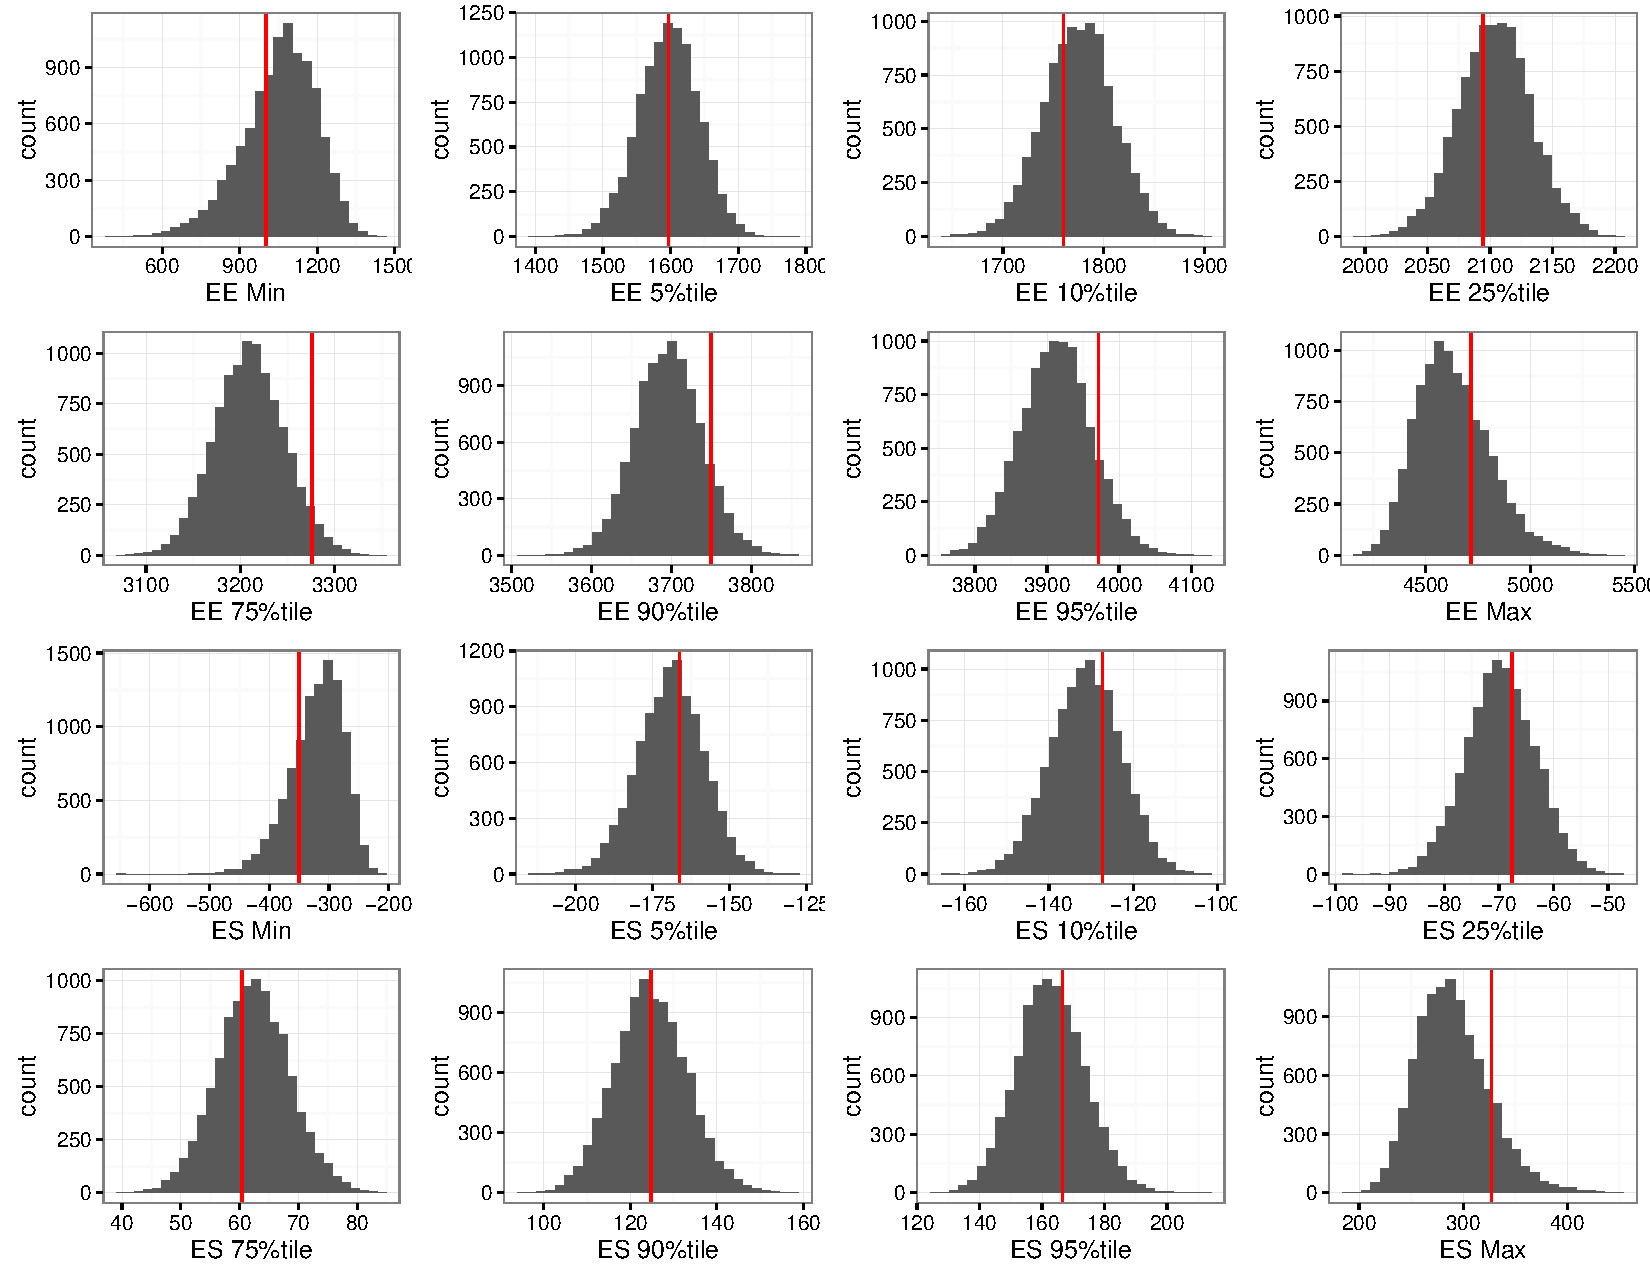
\includegraphics[width=17cm,height=15cm]{manual_figure/wpydiagbvnb.pdf}
%   \caption{Posterior Predictive Discrepancy Measures For $Y^{EE}$ and $Y^{\Delta ES}$ for Model BVN with Bimodal Normal Errors}
%   \label{wpydiagbvnb}
%   \end{figure}
% 
% 
% 
%   \begin{figure}
%   \centering
%   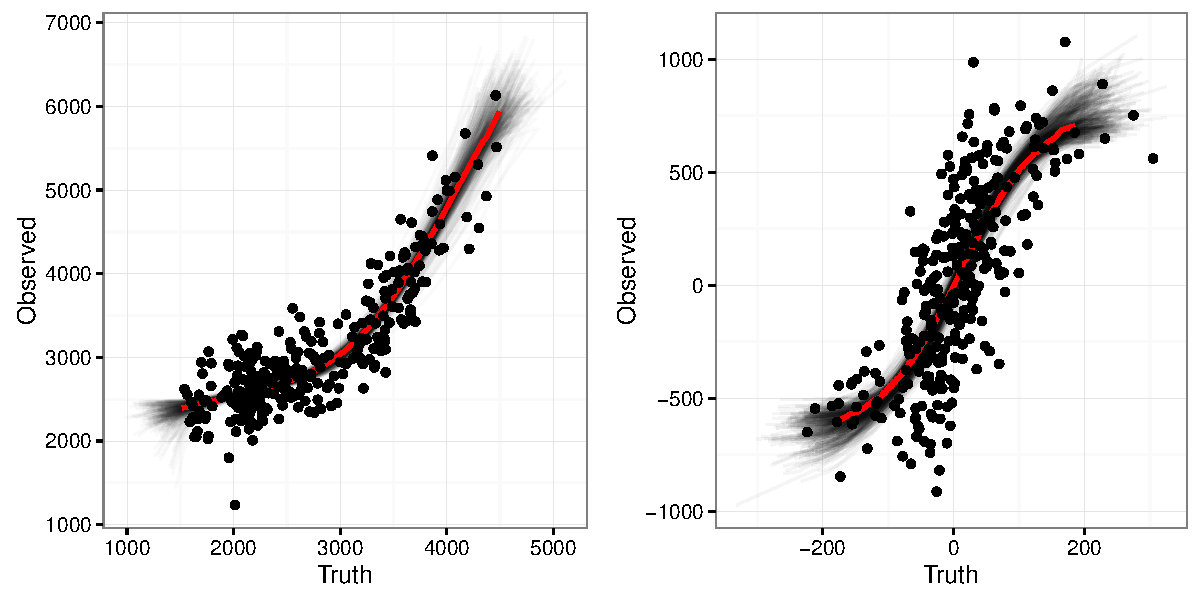
\includegraphics[width=17cm,height=8cm]{manual_figure/predbvnx.pdf}
%   \caption{Spline function for Model BVN with Normal Errors}
%   \label{predbvnx}
%   \end{figure}
% 
%   \begin{figure}
%   \centering
%   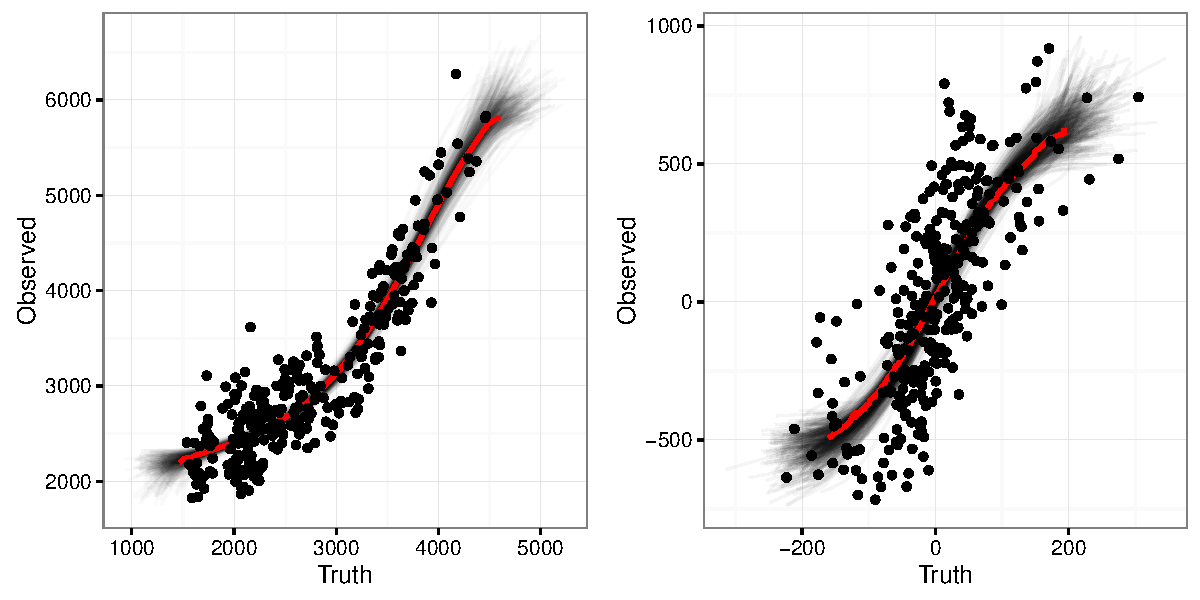
\includegraphics[width=17cm,height=8cm]{manual_figure/predbvnsx.pdf}
%   \caption{Spline function for Model BVN with Skewed Errors}
%   \label{predbvnsx}
%   \end{figure}
% 
%   \begin{figure}
%   \centering
%   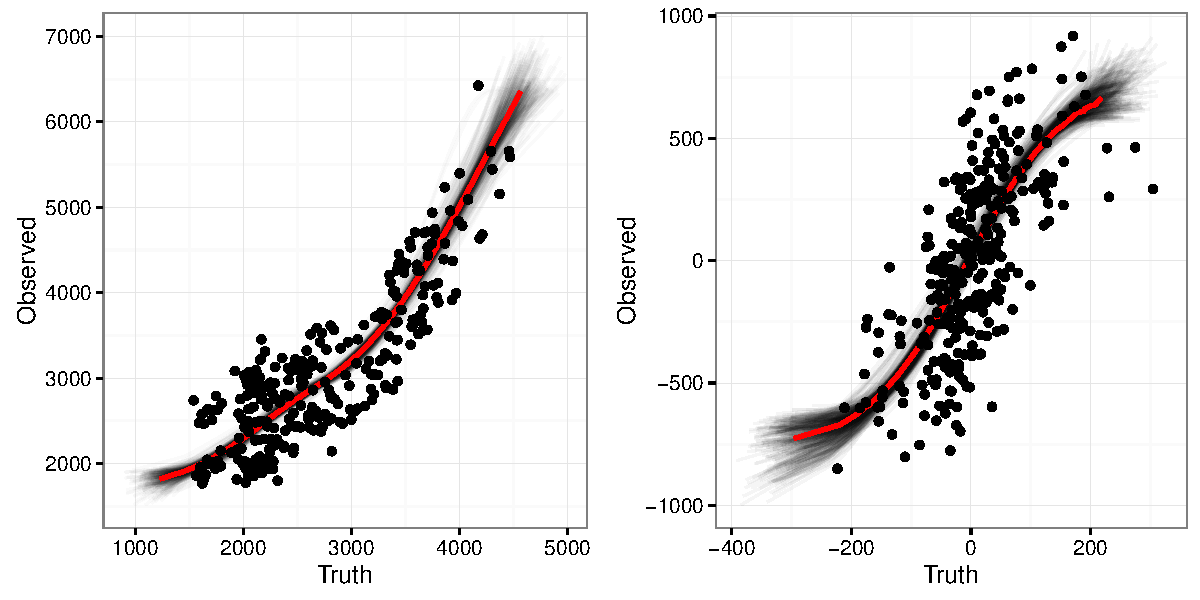
\includegraphics[width=17cm,height=8cm]{manual_figure/predbvnbx.pdf}
%   \caption{Spline function for Model BVN with Bimodal Errors}
%   \label{predbvnbx}
%   \end{figure}

%-------------------------------------------------------------%
%-------------------------------------------------------------%
%--------------------  Model DP
%-------------------------------------------------------------%
%-------------------------------------------------------------%
% 
% 
%--------------------------------------
% \subsection{Model DP}
% %--------------------------------------
% 
% %---------------------------%
% %\subsection{Issues with DP}
% %---------------------------%
% 
% Although we'd like to be as flexible as possible with our distributional assumptions on the bivariate latent variables, we also want a model that is stable in its estimates given the data constraints of our application. It would be difficult to get more than 2 replicate measurements on an individual for our gold standard measurements. For 3 replicate measuremnets in the DLW case, this amounts to three 2-week periods along with a washout time in between. In the case of DXA scans, this is 6 scans in a short period of time which can raise flags due to radiation concerns. This is exemplified by the high cost associated with these methods (mainly DLW). Cheap measuremnet tools are not as much of a concern, but they are biased measuremnets of the latent variables unlike the gold standards. During our simulation study, we found that the DP on the latent variables was producing unstable results in parameter estimates and acceptance rates of the random walk Metropolis-Hastings under 2 replicate observations per person. The number of individuals played a much smaller role. Results were stable when 4 replicates per person were used. Results were similar when we used mixtures of normals instead of a DP. This presents an issue in our analysis since it is unrealistic to get that number of replicates in application. Becuase of this issue, we propose using a bivariate normal distribution for the latent variables. 
% 
% Nonetheless, we show the results from Model DP under a completely unrealistic data collection standpoint by simulating 20 replicates. This gives us the ``best case scenario''. We give results for this model in addition to the rest in the full simulation study. Tables \ref{mdpwpestimates},\ref{mdpswpestimates},\ref{mdpbwpestimates} give posterior quantiles of parameters under normal, skewed, and bimodal errors respectively. Figure \ref{wpxdiagdp} shows posterior predictive assessment of the latent variables. Looking at this plot we see considerable improvement over the model using only a bivariate normal distribution. 
% 
% % 
% % For our model we ran 3 chains of 20,000 iterations with a burn in of 5000 iterations. For the regression and variance components, the Gelman-Rubin diagnostic was less than 1.1 for all parameters and trace plots indicated good mixing. To check for any signs of lack of convergence for the Dirichlet process, we calculated the estimated densities for EE and $\Delta$ES at random locations and compared across iterations and chains. Trace plots indicated good mixing of these densities. We also monitored 
% % 
% \begin{table}[ht]
% \centering
% \begin{tabular}{rrrrrr|r}
%   \hline
%  & 2.5\% & 25\% & 50\% & 75\% & 97.5\% & Truth \\
%   \hline
% $\sigma_{yee}$ & 399.34 & 404.47 & 407.27 & 410.22 & 416.30 \\ 
%   $\sigma_{yes}$ & 334.08 & 338.30 & 340.56 & 342.90 & 347.58 \\ 
%   $\sigma_{wee}$ & 250.89 & 253.97 & 255.63 & 257.27 & 260.49 \\ 
%   $\sigma_{wes}$ & 70.72 & 71.57 & 72.02 & 72.47 & 73.37 \\ 
%   $\gamma_{1,ee}$ & 107.00 & 170.43 & 203.21 & 235.50 & 297.66 \\ 
%   $\gamma_{2,ee}$ & 1.00 & 5.48 & 7.82 & 10.22 & 14.70 \\ 
%   $\gamma_{3,ee}$ & -16.52 & -12.49 & -10.33 & -8.21 & -4.14 \\ 
%   $\gamma_{1,es}$ & -265.69 & -213.87 & -186.87 & -159.35 & -106.99 \\ 
%   $\gamma_{2,es}$ & 1.99 & 5.91 & 7.95 & 9.98 & 13.74 \\ 
%   $\gamma_{3,es}$ & -9.62 & -6.19 & -4.37 & -2.55 & 0.95 \\ 
%    \hline
% \end{tabular}
% \caption{Parameter estimates for Model DP for Normal errors with correct specification of within person errors}
% \label{mdpwpestimates}
% \end{table}
% 
% 
% \begin{table}[ht]
% \centering
% \begin{tabular}{rrrrrr|r}
%   \hline
%  & 2.5\% & 25\% & 50\% & 75\% & 97.5\% & Truth \\
%   \hline
% $\sigma_{yee}$ & 408.76 & 414.08 & 417.00 & 419.99 & 426.09 \\ 
%   $\sigma_{yes}$ & 300.98 & 304.68 & 306.72 & 308.83 & 313.14 \\ 
%   $\sigma_{wee}$ & 248.17 & 251.18 & 252.82 & 254.48 & 257.66 & 250 \\ 
%   $\sigma_{wes}$ & 70.60 & 71.42 & 71.87 & 72.33 & 73.20 & 72.862 \\ 
%   $\gamma_{1,ee}$ & 126.93 & 189.61 & 222.63 & 256.03 & 320.63 & 300 \\ 
%   $\gamma_{2,ee}$ & 1.70 & 6.28 & 8.67 & 11.10 & 15.61 & 14 \\ 
%   $\gamma_{3,ee}$ & -17.74 & -13.65 & -11.39 & -9.30 & -5.12 & -7 \\ 
%   $\gamma_{1,es}$ & -268.29 & -220.21 & -195.87 & -171.08 & -124.51 & -200 \\ 
%   $\gamma_{2,es}$ & 3.00 & 6.43 & 8.22 & 10.04 & 13.47 & 8 \\ 
%   $\gamma_{3,es}$ & -9.25 & -6.16 & -4.50 & -2.88 & 0.23 & -5 \\ 
%    \hline
% \end{tabular}
% \caption{Parameter estimates for Model DP for Skewed errors with correct specification of within person errors}
% \label{mdpswpestimates}
% \end{table}
% 
% \begin{table}[ht]
% \centering
% \begin{tabular}{rrrrrr|r}
%   \hline
%  & 2.5\% & 25\% & 50\% & 75\% & 97.5\% & Truth \\
%   \hline
% $\sigma_{yee}$ & 237.57 & 241.51 & 243.66 & 245.95 & 251.23 \\ 
%   $\sigma_{yes}$ & 240.24 & 243.34 & 245.03 & 246.74 & 250.16 \\ 
%   $\sigma_{wee}$ & 190.56 & 194.04 & 196.34 & 198.77 & 203.20 \\ 
%   $\sigma_{wes}$ & 55.51 & 56.18 & 56.54 & 56.91 & 57.62 \\ 
%   $\gamma_{1,ee}$ & 99.82 & 142.58 & 166.71 & 190.73 & 237.84 \\ 
%   $\gamma_{2,ee}$ & 3.09 & 5.93 & 7.44 & 8.93 & 11.78 \\ 
%   $\gamma_{3,ee}$ & -13.32 & -10.80 & -9.49 & -8.16 & -5.68 \\ 
%   $\gamma_{1,es}$ & -249.38 & -212.33 & -192.64 & -172.90 & -135.52 \\ 
%   $\gamma_{2,es}$ & 4.83 & 7.58 & 9.00 & 10.44 & 13.17 \\ 
%   $\gamma_{3,es}$ & -9.00 & -6.53 & -5.24 & -3.95 & -1.48 \\ 
%    \hline
% \end{tabular}
% \caption{Parameter estimates for Model DP for Bimodal errors with correct specification of within person errors}
% \label{mdpbwpestimates}
% \end{table}
% % 
% % 
% %  %post pred check for X
%  \begin{figure}
%   \centering
%   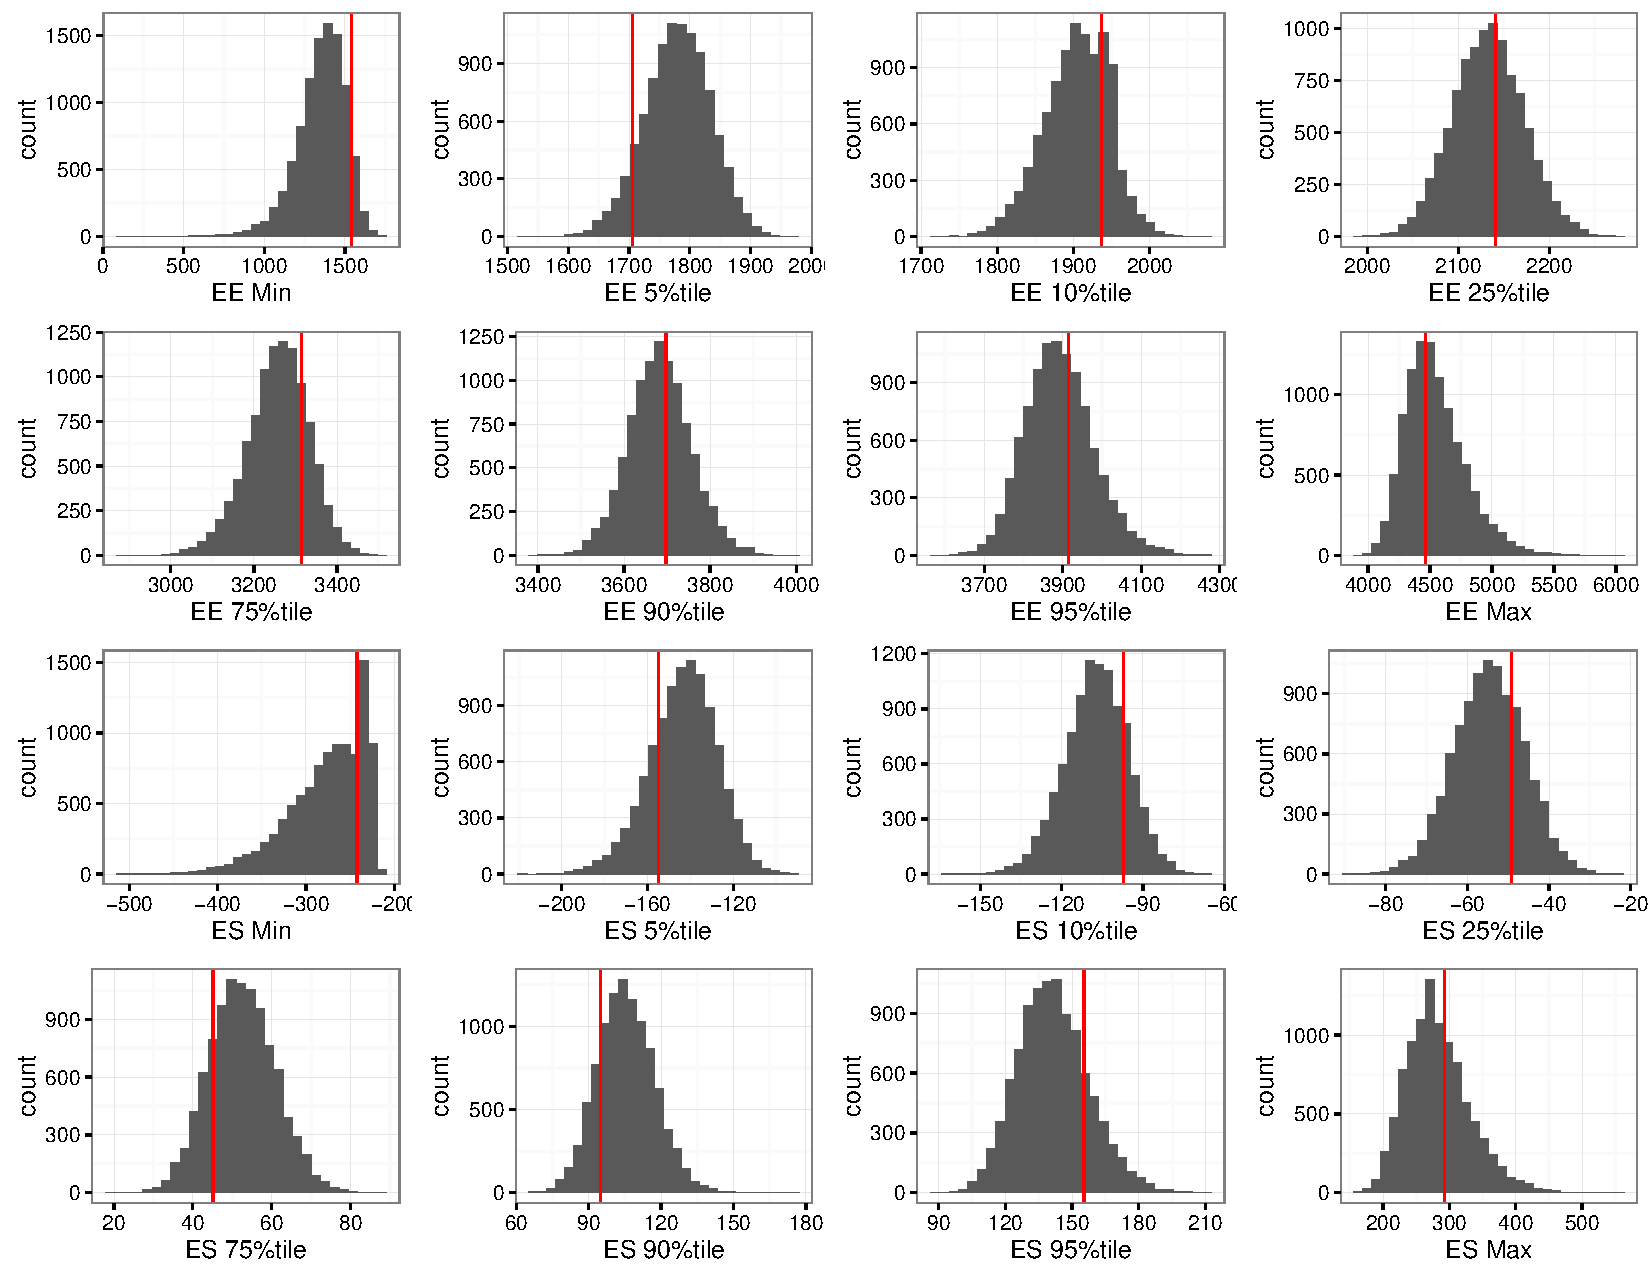
\includegraphics[width=17cm,height=15cm]{manual_figure/wpxdiagdp20.pdf}
%   \caption{Posterior Predictive Discrepancy Measures For $X^{EE}$ and $X^{\Delta ES}$ for Model DP with Normal Errors}
%   \label{wpxdiagdp}
%   \end{figure}
%  %post pred check for W
%   \begin{figure}
%   \centering
%   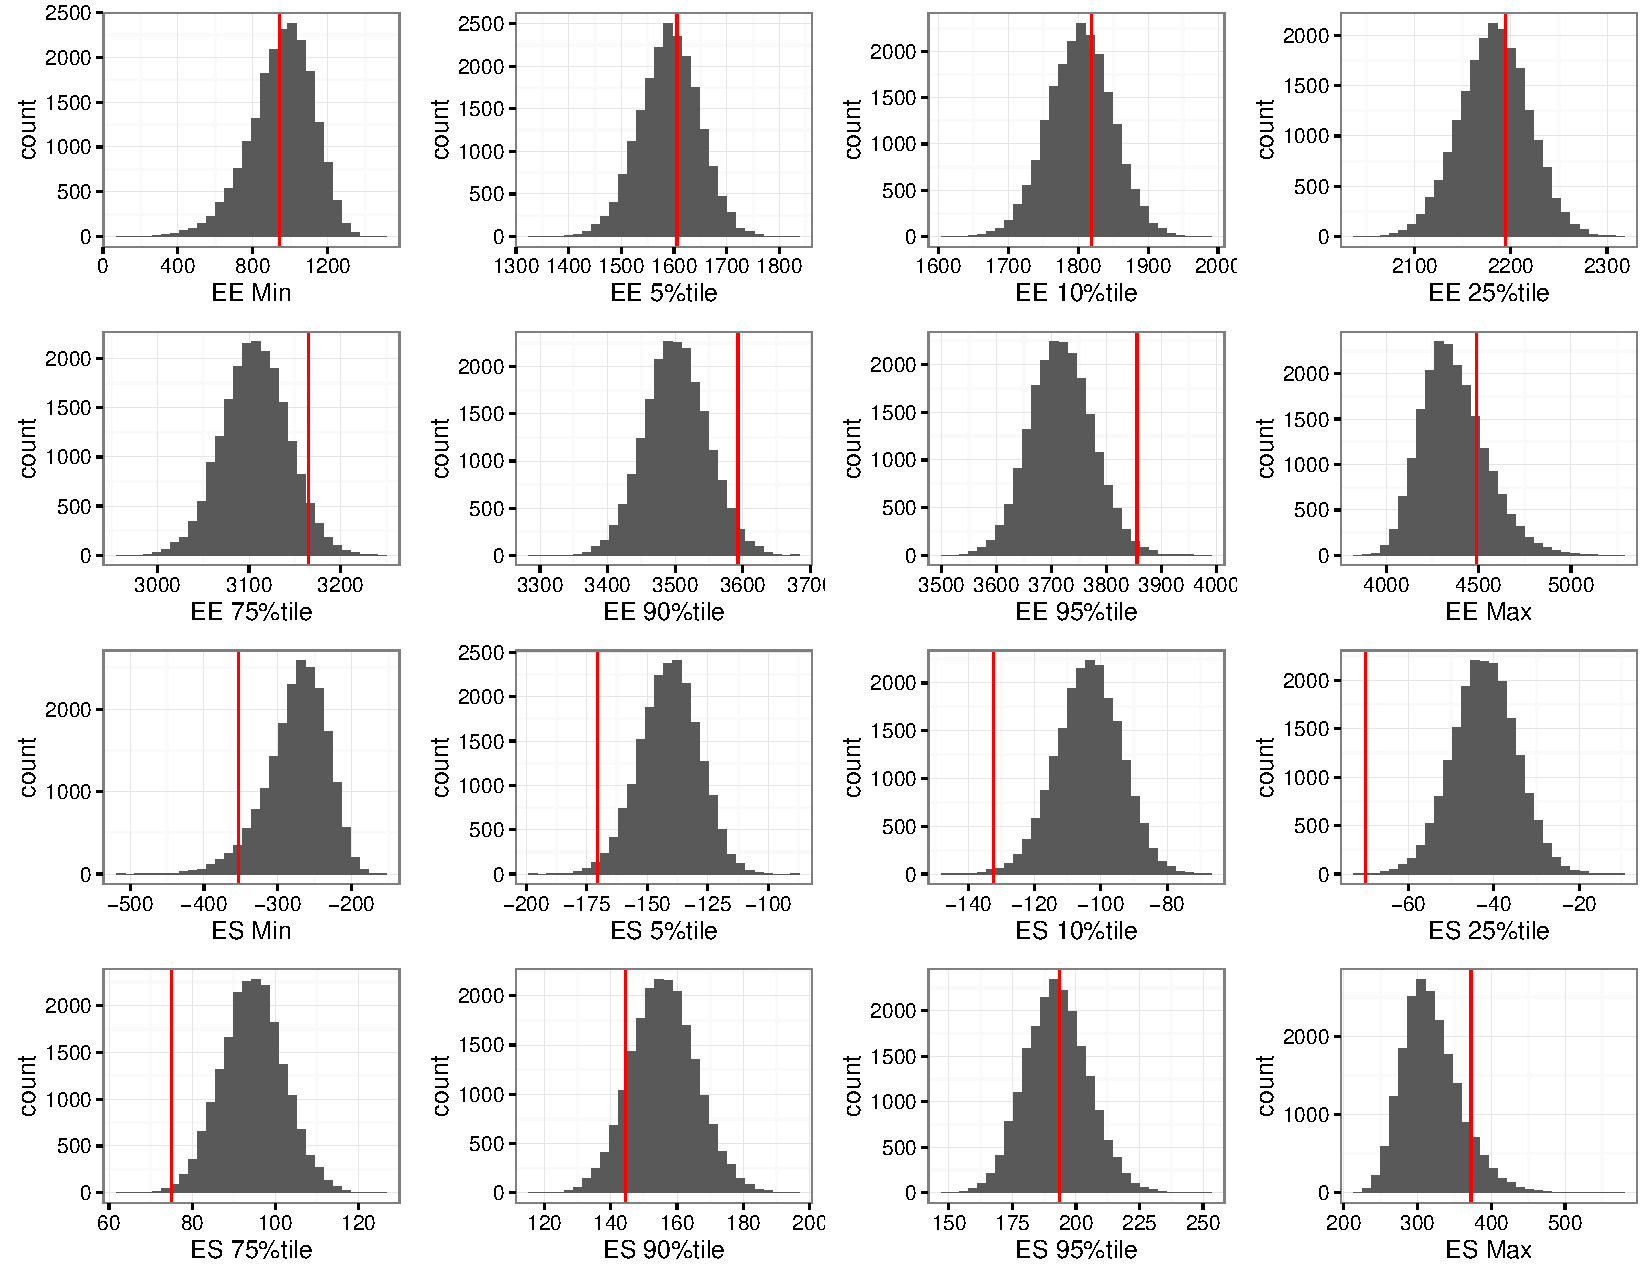
\includegraphics[width=17cm,height=15cm]{manual_figure/wpwdiagdp.pdf}
%   \caption{Posterior Predictive Discrepancy Measures For $W^{EE}$ and $W^{\Delta ES}$ for Model DP with Normal Errors}
%   \label{wpwdiagdp}
%   \end{figure}
%  %post pred check for Y
%   \begin{figure}
%   \centering
%   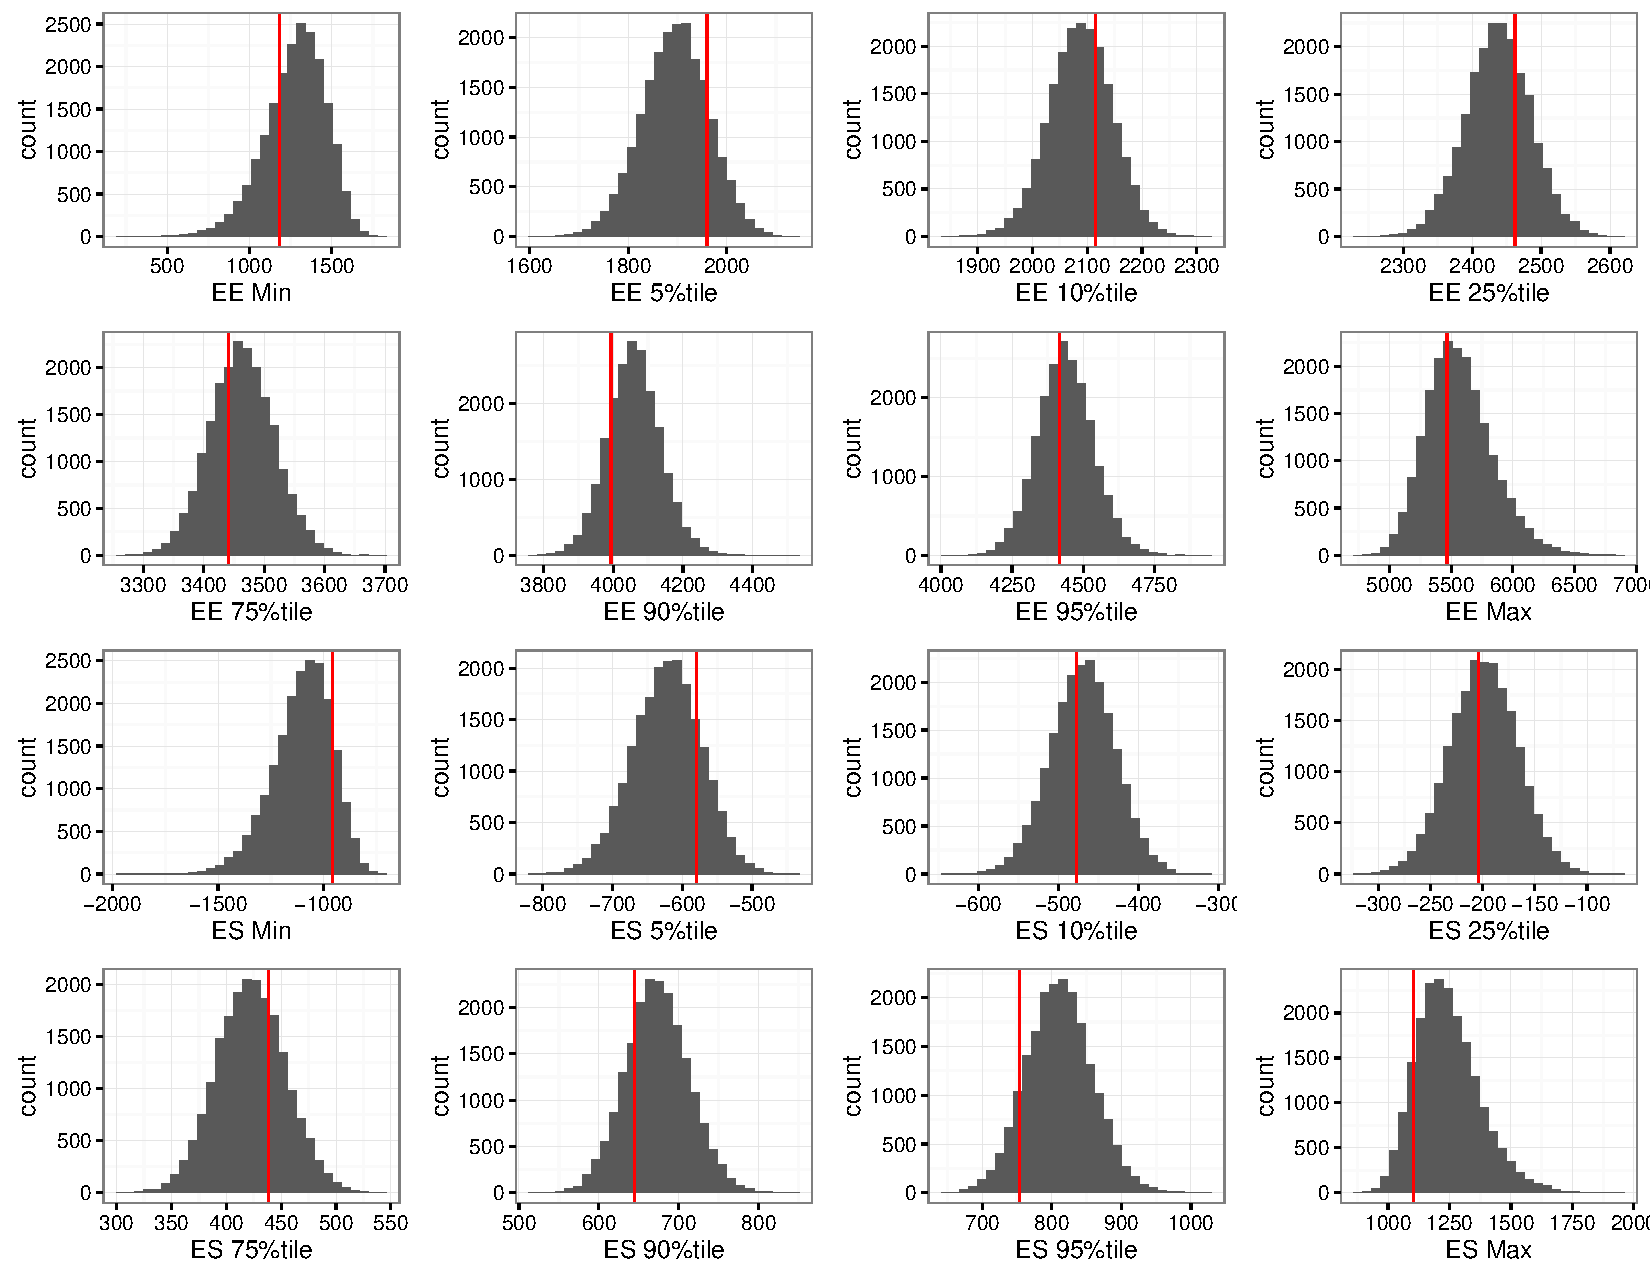
\includegraphics[width=17cm,height=15cm]{manual_figure/wpydiagdp.pdf}
%   \caption{Posterior Predictive Discrepancy Measures For $Y^{EE}$ and $Y^{\Delta ES}$ for Model DP with Normal Errors}
%   \label{wpydiagdp}
%   \end{figure}
% 
% 
%  %post pred check for X
%  \begin{figure}
%   \centering
%   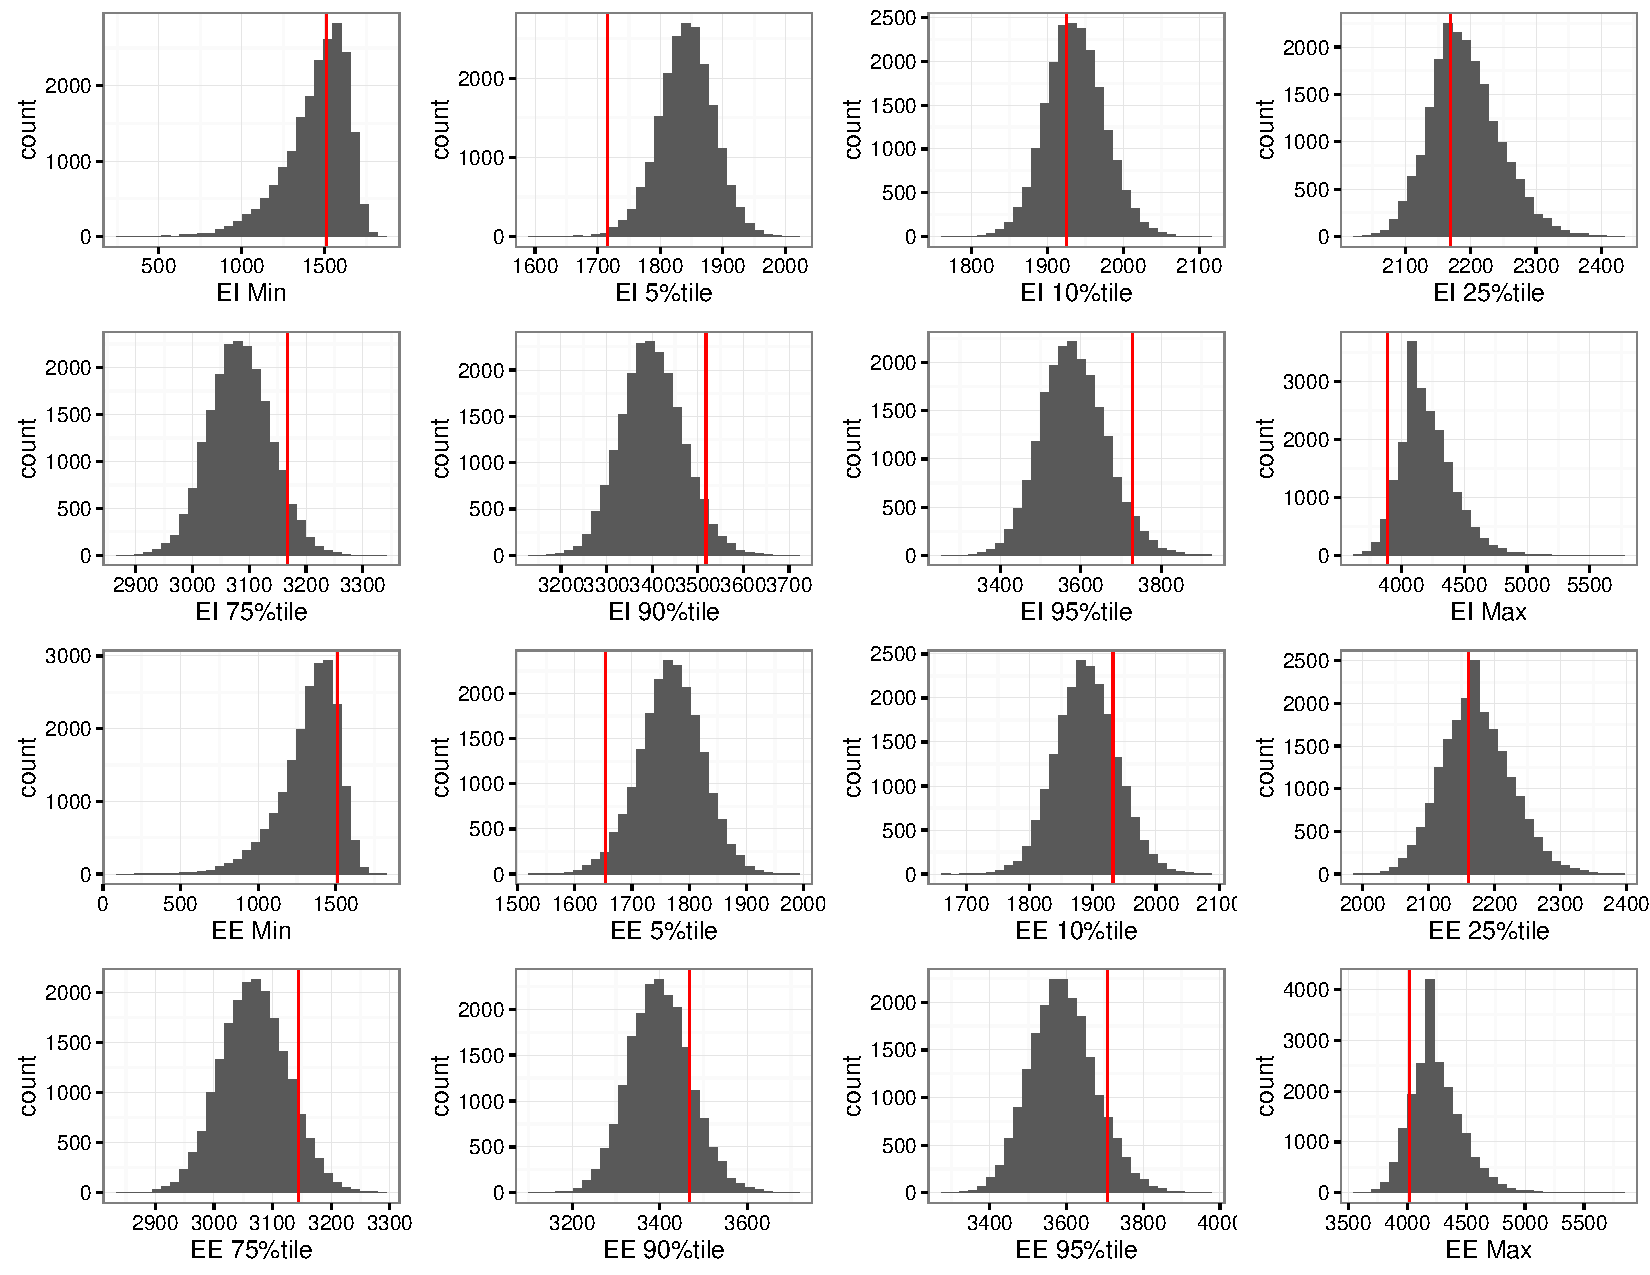
\includegraphics[width=17cm,height=15cm]{manual_figure/wpxdiagdps.pdf}
%   \caption{Posterior Predictive Discrepancy Measures For $X^{EE}$ and $X^{\Delta ES}$ for Model DP with Skewed Normal Errors}
%   \label{wpxdiagdps}
%   \end{figure}
%  %post pred check for W
%   \begin{figure}
%   \centering
%   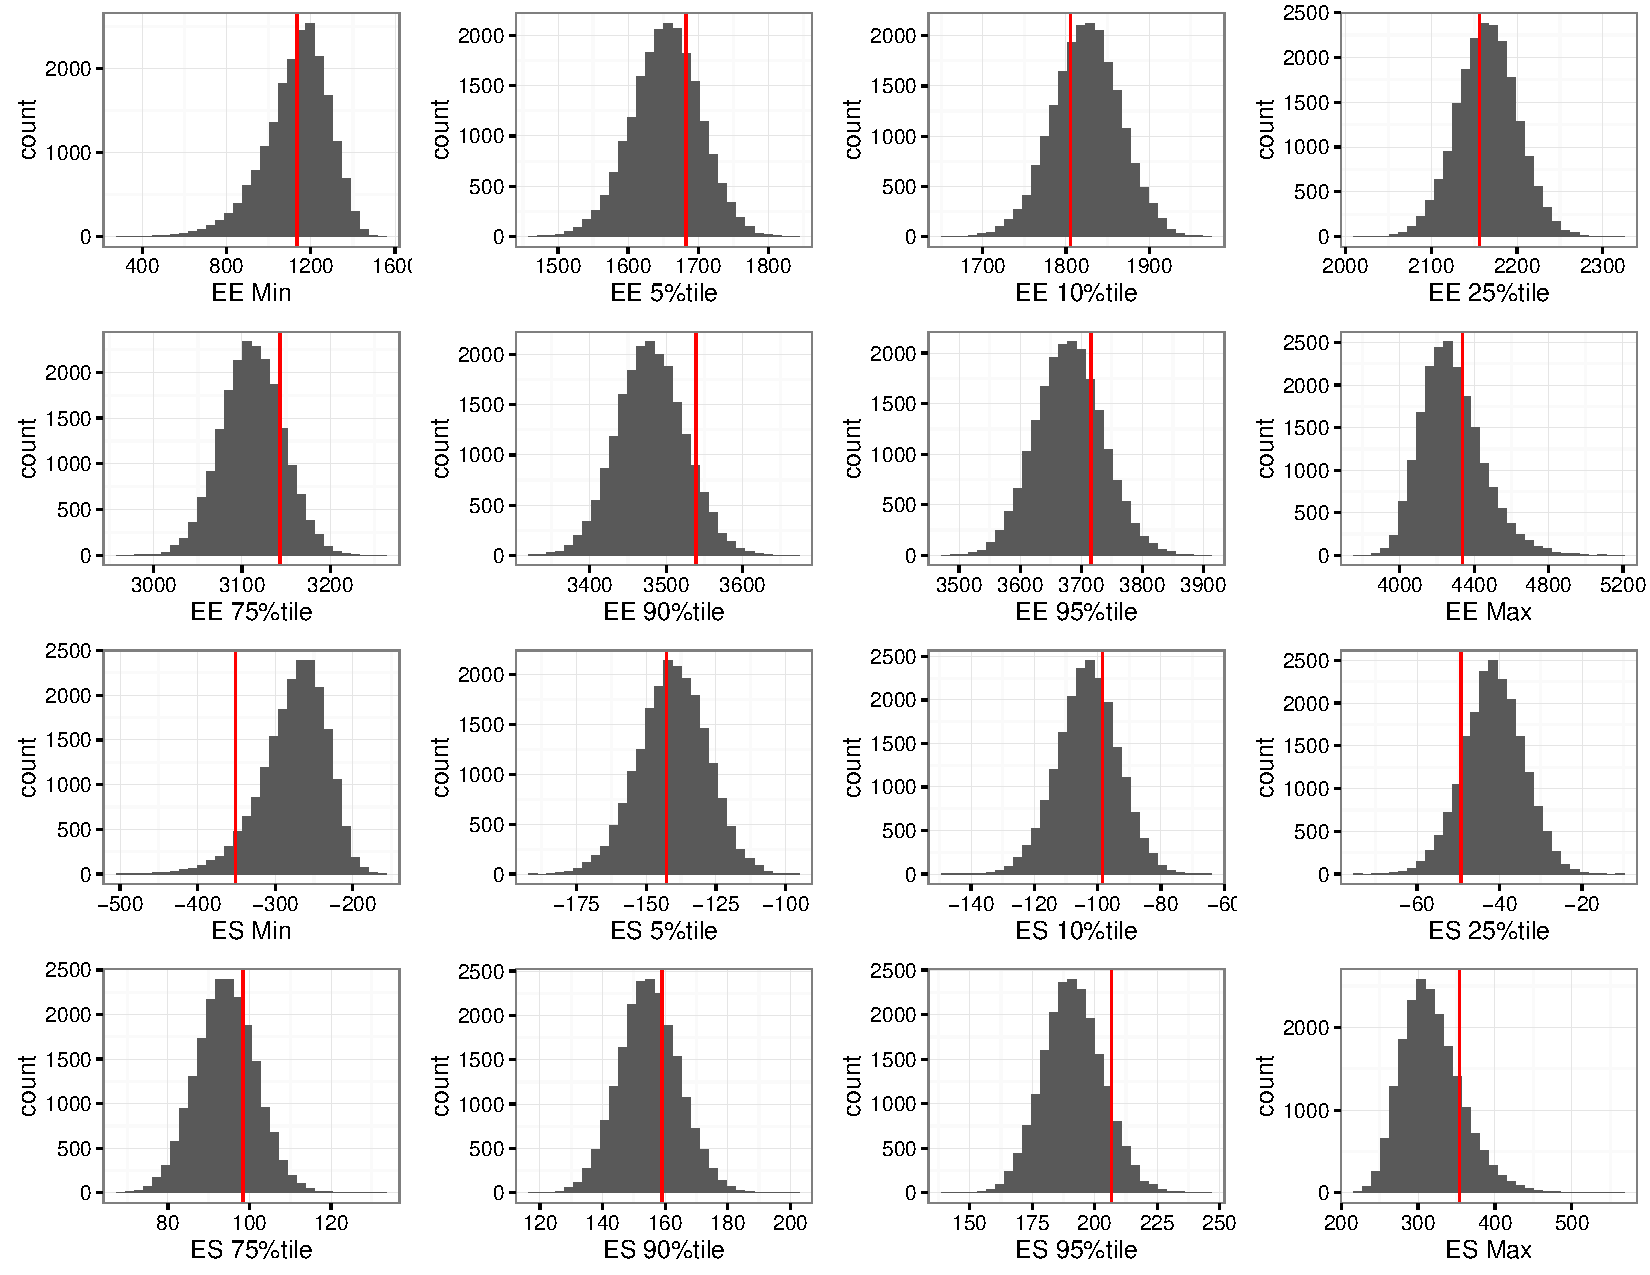
\includegraphics[width=17cm,height=15cm]{manual_figure/wpwdiagdps.pdf}
%   \caption{Posterior Predictive Discrepancy Measures For $W^{EE}$ and $W^{\Delta ES}$ for Model DP with Skewed Normal Errors}
%   \label{wpwdiagdps}
%   \end{figure}
%  %post pred check for Y
%   \begin{figure}
%   \centering
%   \includegraphics[width=17cm,height=15cm]{manual_figure/wpydiagdps.pdf}
%   \caption{Posterior Predictive Discrepancy Measures For $Y^{EE}$ and $Y^{\Delta ES}$ for Model DP with Skewed Normal Errors}
%   \label{wpydiagdps}
%   \end{figure}
%   
% 
% 
%   \begin{figure}
%   \centering
%   \includegraphics[width=17cm,height=8cm]{manual_figure/wppreddp.pdf}
%   \caption{Spline function for Model DP with Normal Errors}
%   \label{wppreddp}
%   \end{figure}

% \begin{table}[ht]
% \centering
% \begin{tabular}{l|rr|rr|rr}
%   \hline
%  & Normal Error & & SN Error & & Bimodal Error & \\ 
%   \hline
%   & EE & $\Delta$ES & EE & $\Delta$ES & EE & $\Delta$ES \\
%   \hline
%   N{\"a}ive Model & 152567 & 57792 & 148931 & 50032 & 102039 & 22365 \\
%   Simple Model & 121385  & 42402 & 103757 & 39278 & 55922 & 19885 \\
%   Our Model & 75488 & 38350 & 73637 & 37313 & 47398 & 18940 \\
%    \hline
% \end{tabular}
% \caption{Mean PMSE for all models under 3 different error distributions using correct within person variability specification}
% \label{pmse2}
% \end{table}


%-------------------------------------------------------------%
%-------------------------------------------------------------%
%-------------------------------------------------------------%
\section{Calibration}
%-------------------------------------------------------------%
%-------------------------------------------------------------%
%-------------------------------------------------------------%

One of the main goals of this research was to provide the best possible estimates of EE and $\Delta$ES using cheap measurement tools. The path we took to create those estimates was by modeling the bias and error in the cheap measurements by using replicates of unbiased gold standard measurements. In this section we describe how we can use our measurement error model to calibrate what a cheap measurement reports for either EE or $\Delta$ES and return a more accurate estimate along with measures of uncertainty. 

Once we have fit our model to a specific set of cheap measurement tools for EE and $\Delta$ES, we can use our model to calibrate measurements from those cheap meaurements in the future. That is, given an estimate of EE or $\Delta$ES from a cheap measurement tool and some demographic information, we can return a better estimate of the truth as well as a credible interval that shows the uncertainty in the estimate. Calibration for our models simply amounts to finding the inverse of the fitted models in \eqref{regressionfcn1}, \eqref{regressionfcn2} as a function of $Y$ instead of $X$, and $Z$ are still measurement error free covariates as shown below.

\begin{align}
  X_{calibrated} &= m^{-1}(y-\boldsymbol{\gamma}' Z) 
\end{align}

We cannot find the inverse of our regression function in closed form so we will find it numerically instead. To do so, we use \texttt{optimize} in \texttt{R} for the function $|f(x)-y^*|$ where $f()$ represents the regression function and $y^*$ is the observed cheap measurement minus the vector of coefficients $\boldsymbol{\gamma}$ multiplied by the individuals covariate values $Z$. We specify a number of posterior draws of regression coefficients and latent variables $R$, to then get a set of predicted values for $X$. We use each of these posterior draws of regression coefficients, latent variables, and spline function to get a calibrated value. Using this set of calibrated values, we can then get a point estimate for the value of $X$ as well as a credible interval using percentiles from the set of estimates. The procedure for getting this distribution for the calibration for individual $i$ is as follows:

For r = 1,...R
\begin{enumerate}
\item
Calculate $y_i^* = y_i- \boldsymbol{\gamma}^{(r)'} Z_i$, where $Z_i$ are the covariate values for individual $i$
\item
Use \texttt{optimize} for the function $|f_i(x) - y_i^*|$ to choose the value of $x$ that will minimize the forementioned criteria, call this $x_{i,calibrated}$. $f_i(x)$ is the predicted value of $y_i$ for the given value $x$ using the MCMC draw for the spline coefficients, latent variables, and knot locations from the $r^{th}$ draw of the chain

\end{enumerate}


As an example, we want to calibrate three cheap measurements each from a different individual using Model BVNS. We randomly select 3 individuals from the same data set used earlier to give results for model BVNS. Individual 1 is female, BMI of 21.9, age 29; individual 2 is female, BMI of 24.9, age 38 and individual 3 is male, BMI 29.2 and age 30. Observed cheap measurements for these individuals, their true values, as well as 95\% credible intervals for their calibrated truth under normal errors are given in Table \ref{calibratedee}. Figures \ref{wpcalhist} gives histograms of 1000 calibrated draws for each individual for EE and $\Delta$ES measurements under skewed errors. 

Looking at the table and figure, one can see that the calibration helps pull the cheap measurement closer to the truth. One can also see that sometimes the cheap measurement is actually close to the truth. What's even more exciting about this is that we have measures of uncertainty immediately, and thus we can get credible intervals easily.

\begin{table}[ht]
\centering
\begin{tabular}{r|ccc|cc}
  \hline
& Lower & Median & Upper & Observed & Truth \\ 
  \hline
EE & 1824.39 & 2041.63 & 2228.32 & 2262.38 & 2204.20 \\ 
  & 3960.54 & 4069.96 & 4216.28 & 4826.14 & 3958.90 \\ 
  & 3305.31 & 3370.59 & 3439.96 & 3567.78 & 3110.84 \\ 
   \hline  
   $\Delta$ES & 182.80 & 238.05 & 426.32 & 643.26 & 200.72 \\ 
  & -14.80 & 10.08 & 37.26 & -163.09 & 5.34 \\ 
  & -488.63 & -230.82 & -170.28 & -904.79 & -252.62 \\
   \hline
\end{tabular}
\caption{95\% credible interval for calibration estimate for cheap EE measurements for Skewed Errors} 
\label{calibratedee}
\end{table}


% \begin{table}[ht]
% \centering
% \begin{tabular}{ccc|c}
%   \hline
% 2.5\% & 50\% & 97.5\% & Observed \\ 
%   \hline
% 2164.46 & 2270.61 & 2358.48 & 2500.00 \\ 
%   2610.96 & 2730.93 & 2838.02 & 3200.00 \\ 
%   3365.49 & 3460.00 & 3546.59 & 4000.00 \\ 
%    \hline
% \end{tabular}
% \caption{95\% credible interval for calibration estimate for cheap EE measurements with Skewed Errors} 
% \label{calibratedees}
% \end{table}
% 
% 
% \begin{table}[ht]
% \centering
% \begin{tabular}{ccc|c}
%   \hline
% 2.5\% & 50\% & 97.5\% & Observed \\ 
%   \hline
% -5.94 & 58.12 & 126.48 & -250.00 \\ 
%   -325.05 & -197.91 & -63.23 & 320.00 \\ 
%   77.93 & 143.46 & 212.29 & 90.00 \\ 
%    \hline
% \end{tabular}
% \caption{95\% credible interval for calibration estimate for cheap $\Delta$ES measurements with Skewed Errors} 
% \label{calibratedess}
% \end{table}
% 
% 
% \begin{table}[ht]
% \centering
% \begin{tabular}{ccc|c}
%   \hline
% 2.5\% & 50\% & 97.5\% & Observed \\ 
%   \hline
% 2314.13 & 2372.62 & 2425.64 & 2500.00 \\ 
%   2644.81 & 2732.56 & 2811.99 & 3200.00 \\ 
%   3369.09 & 3432.99 & 3503.77 & 4000.00 \\ 
%    \hline
% \end{tabular}
% \caption{95\% credible interval for calibration estimate for cheap EE measurements for Bimodal Errors} 
% \label{calibratedeeb}
% \end{table}
% 
% \begin{table}[ht]
% \centering
% \begin{tabular}{ccc|c}
%   \hline
% 2.5\% & 50\% & 97.5\% & Observed \\ 
%   \hline
% 1.78 & 49.83 & 102.56 & -250.00 \\ 
%   -246.29 & -150.32 & -52.08 & 320.00 \\ 
%   82.82 & 140.38 & 201.24 & 90.00 \\ 
%    \hline
% \end{tabular}
% \caption{95\% credible interval for calibration estimate for cheap $\Delta$ES measurements for Bimodal Errors} 
% \label{calibratedesb}
% \end{table}

  % \begin{figure}
  % \centering
  % \includegraphics[width=17cm,height=8cm]{manual_figure/wpcal.pdf}
  % \caption{gghjghj}
  % \label{cal}
  % \end{figure}
  
  %   \begin{figure}
  % \centering
  % \includegraphics[width=17cm,height=8cm]{manual_figure/wpcals.pdf}
  % \caption{dfgd}
  % \label{cals}
  % \end{figure}
  
  %   \begin{figure}
  % \centering
  % \includegraphics[width=17cm,height=8cm]{manual_figure/wpcalb.pdf}
  % \caption{ftghdth for Model BVN with Bimodal Errors}
  % \label{calb}
  % \end{figure}
  
  
  \begin{figure}
  \centering
  \includegraphics[width=17cm,height=10cm]{manual_figure/wpcalhist.pdf}
  \caption{Posteriors of calibrated observations. Vertical line shows observed value from cheap measurement.}
  \label{wpcalhist}
  \end{figure}
  
  %   \begin{figure}
  % \centering
  % \includegraphics[width=17cm,height=8cm]{manual_figure/wpcalhists.pdf}
  % \caption{gghjghj}
  % \label{df}
  % \end{figure}
  
  %     \begin{figure}
  % \centering
  % \includegraphics[width=17cm,height=10cm]{manual_figure/wpcalhistb.pdf}
  % \caption{gghjghj}
  % \label{dfsr}
  % \end{figure}
  
  
  
%---------------------------------------------------%
%---------------------------------------------------%
\section{Discussion}
%---------------------------------------------------%
%---------------------------------------------------%

In this chapter we presented a semi-parametric model for the measurement of EE and $\Delta$ES. We assume gold standard measurements are unbiased to the truth while cheap measurements are some functions of the truth which we use splines to evaluate, plus a linear combination of demographic, error free covariates. This allows a very flexible relationship between a cheap measurement and its unobserved truth. We assumed normality for measurement error distributions which was justified through the use of diagnostics recommended by Caroll et al. We assumed gold standard measurements and cheap measurements were conditionally independent within and between each other given the latent vector $(X^{EE},X^{\Delta ES})$. We modeled the latent vector $(X^{EE},X^{\Delta ES})$ with both a bivariate normal distribution as well as a Dirichlet process. Although the Dirichlet process was flexible and a much weaker assumption, it required more replicate observations (mainly on gold standard measurements) than is feasible in order to give stable results. The normality assumption was able to give stable and surprisingly good results given the true structure of the latent variables. Because this model was able to stable and pleasing results under the constraint of only two replicates of gold standard measurements, we believe this is the best model for this specific application unless more than 2 replicates per person are available. The resulting estimates, posterior predictive checks, and PMSE show the superiority of our model to a simpler linear measurement error model and the n{\"a}ive model that doens't take measurement error into consideration. 

The main motivation for constructing this model was to model the error and bias in measurements so one can calibrate a cheap measurement tool's output in order to make it closer to the truth. We presented a simple way to do this calibration given a cheap measuremet for EE and $\Delta$ES and values for gender, BMI, and age. Using a Bayesian approach we are easily able to get a posterior distribution for the calibrated estimate which provides a measure of uncertainty. Our example shows that in some cases this calibrated estimate could be far from the observed cheap measurement. 


Further considerations to the model would include allowing for nonconstant variance. At the time we have limited data from a limited number of EE and $\Delta$ES measurement tools, but it is possible nonconstant variance will be an issue for some and not others. We saw some signs of this already as the SWA armband showed signs of nonconstant variance while DXA did not. In this research we opted to assume constant variance for simplicity, but an extension to allow for this would not be difficult. Other measurement error free covariates could be easily added to the regression functions in \eqref{regressionfcn1},\eqref{regressionfcn2} if desired. Revisting the conditional independence assumptions could provide additional improvements, especially the last two. We modeled the bivariate latent variables jointly but random variables $Y^{EE}$ and $W^{EE}$ were assumed to be conditionally independent of $X^{\Delta ES}$ and vice versa, but there could be a relationship there to take advantage of. We performed the same analysis assuming complete independence of EE and $\Delta$ES and there was much more uncertainty in estimates, we anticipate modeling more of the dependence will only help. We assumed normality for our measurement errors which based on diagnostics from the EBS, looked good, however there are more flexible options available, for example Sarkar et al. We are not able to split within person variability and measurement error explicitly which would be desireable for fully understanding the random error associated with a measurement device. Furthermore, we are considering both within person variability and measurement error to be additive in the cheap measurement case which is of course not true, it has a complicated relationship through our estimated functions $m_{\cdot}(\cdot)$. These last issues will be difficult to fix because we would need additional replicate data and there's no way to exactly decouple the relationship within the B-spline.


\clearpage
\bibliographystyle{unsrt} %style of bibliography
\bibliography{referencesebmodels} %tells BibTeX to create a list of references using

\end{document}
